\documentclass[titlepage]{article}
\usepackage[spanish,es-tabla]{babel}

% Set page size and margins
% Replace `letterpaper' with `a4paper' for UK/EU standard size
\usepackage[a4paper,top=2cm,bottom=2cm,left=3cm,right=3cm,marginparwidth=1.75cm]{geometry}

% DIBUJOS
\usepackage{amsmath}
\usepackage{graphicx}
\usepackage[
	colorlinks=true, 
	citecolor=blue, 
	linkcolor=black,
	urlcolor=blue
]{hyperref}

\usepackage{graphicx}
\usepackage{relsize}

%%TABLES
\usepackage{colortbl}
\usepackage{hhline}
\usepackage{color}
\usepackage{tabularray}
\usepackage[table,xcdraw]{xcolor}
\usepackage{longtable}

%%ÍNDICE
\usepackage{titlesec}
\usepackage{blindtext}

%%PSEUCODE
\usepackage[spanish, linesnumbered,ruled,vlined]{algorithm2e}

%%%CODE
\usepackage{listings}

%%BIBLIOGRAFIA
\usepackage{apacite}
\AtBeginDocument{
	\renewcommand{\BRetrievedFrom}{}
}	
\bibliographystyle{apacite}

%%INTERLINEADO DOBLE
\renewcommand{\baselinestretch}{2}

%%INTERLINEADO EN BLOQUES CONCRETOS
\usepackage{setspace}

%%FOOTNOTES
\usepackage[para, multiple,bottom]{footmisc}
\setlength{\skip\footins}{1cm}
\renewcommand{\footnotesize}{\scriptsize}

%%IN-LINE CODE
\usepackage{listings}
\usepackage{color}

%%GRAFICOS
\usepackage{pgfplotstable}


%%---TIMES NEW ROMAN---
\usepackage{mathptmx} % Usa Times New Roman para texto y matemáticas 
\usepackage[utf8]{inputenc} % Manejo de caracteres UTF-8 
\usepackage[T1]{fontenc} % Codificación de fuentes

%%---LANDSCAPE---
\usepackage{lscape}

\lstset{frame=tb,
  language=Java,
  aboveskip=3mm,
  belowskip=3mm,
  showstringspaces=false,
  columns=flexible,
  basicstyle={\small\ttfamily},
  numbers=none,
  numberstyle=\tiny\color{gray},
  keywordstyle=\color{blue},
  commentstyle=\color{dkgreen},
  stringstyle=\color{mauve},
  breaklines=true,
  breakatwhitespace=true,
  tabsize=3
}

%%INFORMACIÓN
\title{¿En qué medida las técnicas de concurrencia optimizan el algoritmo de ordenación Merge Sort?}

%%% UNICODE
\usepackage[utf8]{inputenc}

%%%PGFPLOTS
\usepackage{pgfplots}
\pgfplotsset{compat=1.18}
%%%%CAPTION
\usepackage{caption}

%%%%%FIGURAS ADAPTADAS
\usepackage{wrapfig}

%%%%%Forzar figuras con H
\usepackage{float}

\usetikzlibrary{positioning}

%%APPENDICES
\usepackage{appendix}

\begin{document}
	
\definecolor{dkgreen}{rgb}{0,0.6,0}
\definecolor{gray}{rgb}{0.5,0.5,0.5}
\definecolor{mauve}{rgb}{0.58,0,0.82}	
	
%%%%PORTADA%%%%%%%%%%%%%%%%%
\begin{titlepage}
	\centering
	\hfill
	\vspace{3cm}
	
	\hrule
	\vspace{1cm}
	\onehalfspacing
	{\Huge Impacto de la concurrencia en el rendimiento del algoritmo de ordenación \textit{Merge Sort}\par}
	\vspace{1cm}
	\hrule
	
	\vspace{1cm}
	{\LARGE ¿En qué medida las técnicas de concurrencia del lenguaje de programación Java optimizan el \textit{Merge Sort} recursivo e iterativo? \par}
	
	\vspace{1cm}
	
	{\scshape\large Monografia de Informática\par}
	
	\vspace{8cm}
	
	{\large Cómputo de palabras: 3993\par}
	{\large Código del alumno: lqv708 \par}
	
	
\end{titlepage}

\newpage
\tableofcontents

\newpage
%%%%%%%%%%%%%%%INTRODUCIÓN%%%%%%%%%%%%%%%%%%%%%%
%%%%%%%%%%%%%%%%%%%%%%%%%%%%%%%%%%%%%%%%%%%%%%%%
\section{Introducción} %%248 palabras + 2
Frecuentemente usamos estructuras de datos ordenadas, como la lista de contactos del teléfono, en los almacenes para la gestión de inventario, en los resultados de una búsqueda en internet... El proceso de colocar datos en un cierto orden se llama ordenación y es una operación común en los sistemas informáticos, ya que facilita su búsqueda posterior.\footnote{\cite{knuth-1997}} Aunque, la ordenación ha sido ampliamente estudiada, no existe un algoritmo de ordenación perfecto.\footnote{\cite{McMillan-2007}} Actualmente, se siguen desarrollando, y además relacionan una variedad de conceptos informáticos, como la concurrencia, el paralelismo, la ejecución serial, la iteración o la recursión. Algunos algoritmos de ordenación comunes son la ordenación de burbuja, por inserción, o el ordenamiento rápido.\footnote{\cite{pandey-2008}}

La finalidad de esta investigación es evaluar cuatro implementaciones del algoritmo de ordenación \textit{Merge Sort} en términos de \textbf{complejidad temporal} y \textbf{tiempos de ejecución} reales, además, de la naturaleza específica de cada implementación; con el objetivo de responder a la pregunta <<¿En qué medida las técnicas de concurrencia del lenguaje de programación Java optimizan el \textit{Merge Sort} recursivo e iterativo?>>. Concretamente, se comparan el Merge Sort Iterativo Serial (MSIS) y el Merge Sort Recursivo Serial (MSRS) con sus equivalentes paralelos: Merge Sort Recursivo Paralelo (MSRP) y Merge Sort Iterativo Paralelo (MSIP).

La evaluación se compone de un \textit{análisis a priori}, basado en la estructura de cada algoritmo sin ejecutarlo y calculando un rendimiento esperado; y de un \textit{análisis a posteriori}, enfocado en medir el rendimiento de un algoritmo para una muestra concreta.\footnote{\cite{shoolini2025}}

\subsection{\textit{Merge Sort}} %% 62 palabras +3

\begin{wrapfigure}{r}{0.35\textwidth}
	\vspace{-10pt}
	\centering
	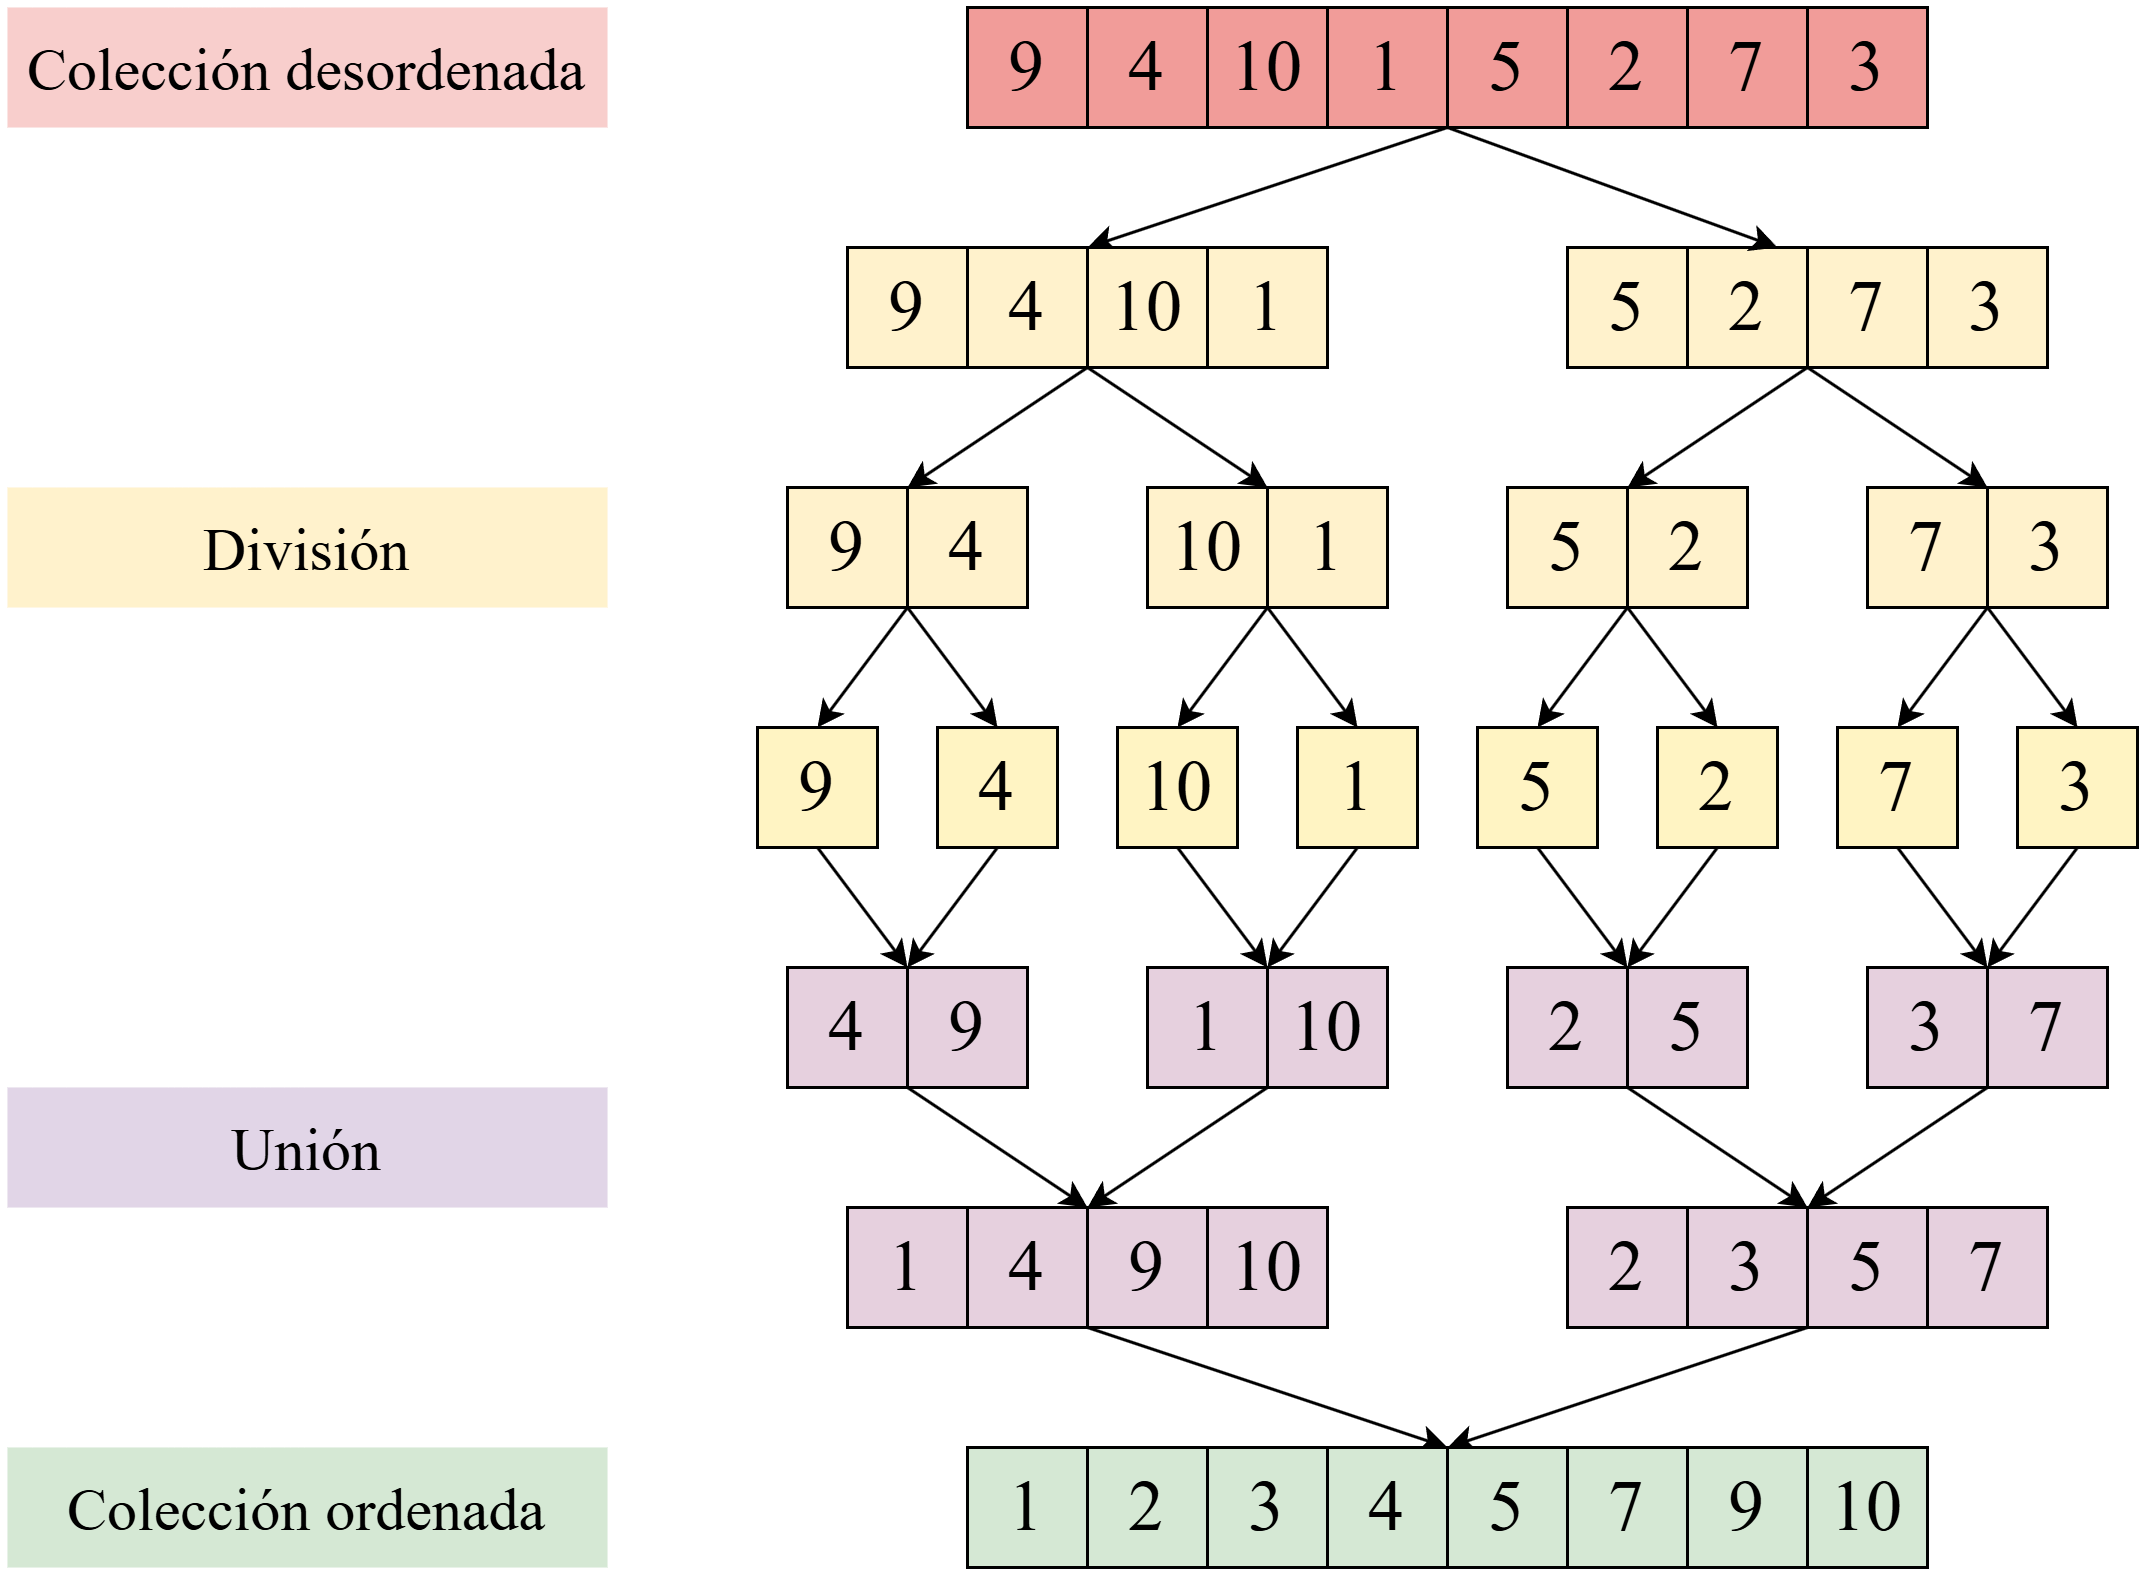
\includegraphics[width=0.35\textwidth]{Diagrames/arbolMS.png}
	\captionsetup{justification=centering}
	\caption{Funcionamiento del \textit{Merge Sort}}
	\label{fig:arbolMS2}
\end{wrapfigure}
El ordenamiento por mezcla es un algoritmo basado en la técnica divide y vencerás. Permite ordenar un conjunto de datos a través de, primero, dividir la colección en dos mitades; dividir las sub-colecciones en más mitades hasta que contengan cero o un elemento; ordenar cada una; y, finalmente, unir ordenadamente todas las sub-colecciones, quedando ordenada la colección entera.\footnote{\cite{skiena-2008}}

\subsection{Ejecución serial y paralela} %% 100 +5
Un \textbf{programa informático} es un conjunto de instrucciones que un sistema informático ejecuta. A su vez, un programa se divide en partes más pequeñas e independientes que llamamos tareas. Cuando las tareas se ejecutan una tras otra durante períodos de tiempo no superpuestos, hablamos de \textbf{ejecución serial}. En contraposición, la \textbf{ejecución paralela} consiste en ejecutar varias tareas simultáneamente. Sin embargo, el paralelismo real solo es posible si el sistema consta de más de una unidad de procesamiento y si las tareas del algoritmo son independientes.\footnote{\cite{bobrov-2023}} Este estudio pretende aplicar el paralelismo a la ordenación por mezcla para aumentar su eficiencia.

\begin{figure}[h]
    \centering
    \captionsetup{justification=centering}
    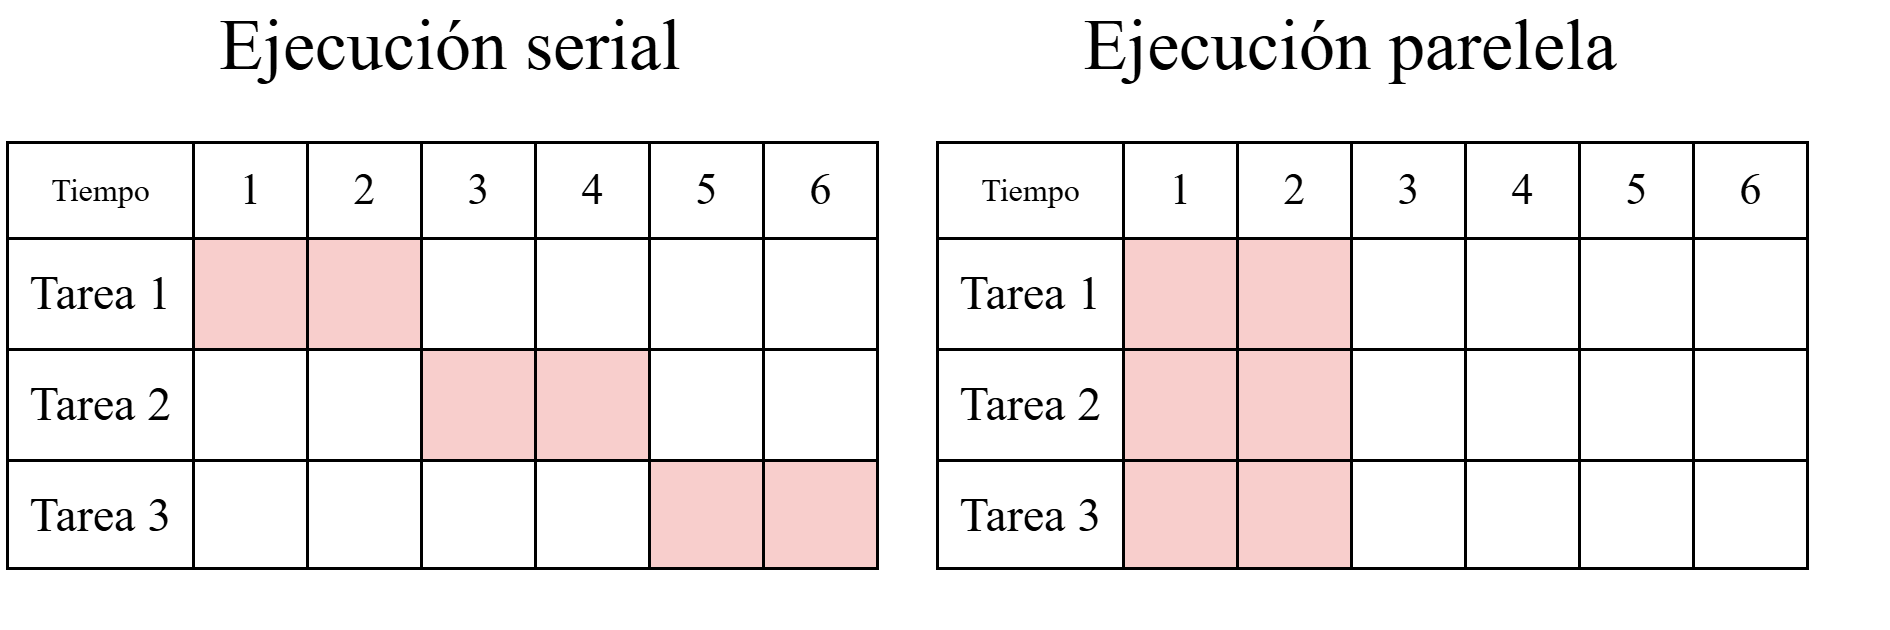
\includegraphics[width=0.85\linewidth]{Diagrames/serialVsParallel.png}
    \caption{Comparación de los diagramas de Gantt}
    \label{fig:serialVsParallel}
\end{figure}

\subsection{Iteración y recursividad} %%77 +4
El paradigma de la \textbf{programación estructurada} considera que todo programa informático está formado por las estructuras de control de Secuencia, Selección y Repetición.\footnote{\cite{extended-learning-institute-no-date}} La recursión es una estructura de repetición.\footnote{\cite{wellesley-college-2000}} Si un programa incorpora una estructura recursiva, quiere decir que hay una función que se llama a sí misma. \footnote{\cite{bhargava-2016}} Toda función recursiva contiene caso recursivo, estructura condicional que llama a la propia función, y un caso base,  que retorna un valor constante o finaliza la función.
\begin{figure}[h]
	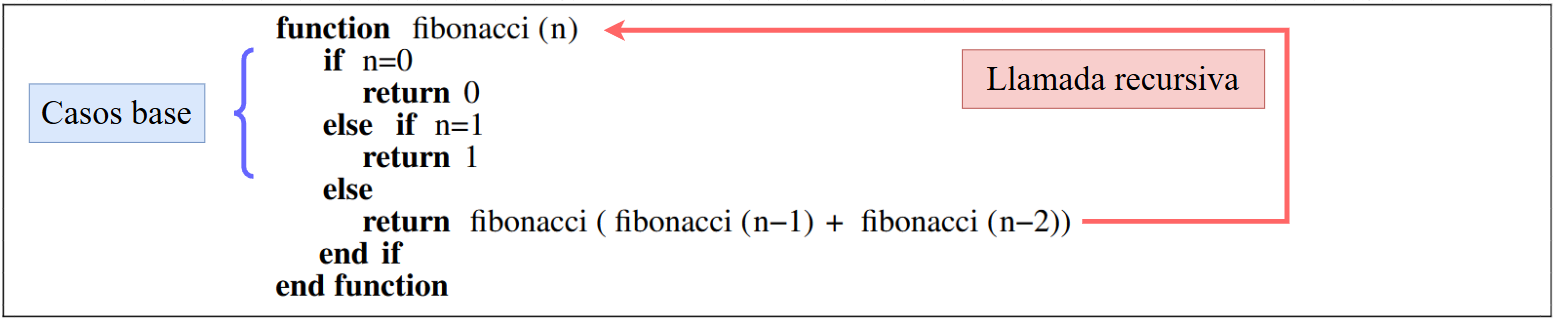
\includegraphics[width=\textwidth]{ejemploRecursion.png}
	
	\label{fig:ejemploRecursion}
\caption{Ejemplo de recursión: sucesión de Fibonacci}

\end{figure}


\subsection{Complejidad} %%197 +2
La eficiencia de un algoritmo de ordenación usualmente se cuantifica en términos de complejidad temporal y espacial.\footnote{\cite{molluzzo1997first}} La complejidad temporal es una medida de la variación del tiempo de ejecución de un algoritmo a medida que el tamaño de la entrada $n$ crece.\footnote{\cite{ching2023uncertainty}} En el caso de un algoritmo de ordenación es la longitud del arreglo.

Puesto que el tiempo de ejecución se ve afectado por variables como el soporte físico y lógico se estudia el comportamiento asintótico: cuando $n$ tiende al infinito. Este método permite comparar algoritmos entre plataformas distintas.\footnote{\cite{Heineman2008-mw}}

Caracterizar un algoritmo por medio de su complejidad es una abstracción basada en la suposición de que las operaciones básicas duran una unidad de tiempo y que cada línea de código es una instrucción básica. Los bucles y llamadas a funciones se evalúan sumando sus instrucciones básicas.\footnote{\cite{datacamp2024bigO}}

	\begin{figure}[h]
		\centering
		\captionsetup{justification=centering}
		\begin{minipage}{0.49\textwidth}
			\centering
			\begin{tikzpicture}
				\begin{axis}[
					xlabel={Entrada $n$},
					ylabel={Tiempo de ejecución},
					xmin=0, xmax=8,
					ymin=0, ymax=5,
					grid=both,
					xtick=\empty,
					ytick=\empty,
					]
					
					\addplot[
					domain=0:8, 
					samples=100, 
					color=blue,
					line width=1pt
					]
					{0.06816*x^5 - 1.25301*x^4 + 8.58526*x^3 - 26.82104*x^2 + 37.54837*x - 17.12774};
					
					\node[right] at (axis cs:6,3) {$f(n)$};
					
					\addplot[
					domain=0:8, 
					samples=100, 
					color=red,
					line width=1pt
					]
					{0.5*x^2 + 0.25*x - 1};
					
					\node[right] at (axis cs:5.5,1.5) {$\Omega(f(n))$};
					
					\addplot[
					domain=0:8, 
					samples=100, 
					color=green,
					line width=1pt
					]
					{-0.00556*x^2 + 0.14167*x + 0.43056};
					
					\node[right] at (axis cs:3.2,4.5) {$O(f(n))$};
					
					\addplot[ 
					color=black, dashed, thick 
					] coordinates{(2,0) (2,1.5)};
				\end{axis}
			\end{tikzpicture}
			\caption{Función de ejemplo \(f(n)\) acotada superiormente por \(O(n)\) y inferiormente por \(\Omega(n)\)}
		\end{minipage}
		\hfill
		\begin{minipage}{0.49\textwidth}
			\centering
			\setlength{\abovecaptionskip}{0.1pt}
			\captionsetup{justification=centering}
			\begin{tikzpicture}
				\begin{axis}[
					xlabel={Entrada $n$},
					ylabel={Tiempo de ejecución},
					restrict y to domain=0:10,
					restrict x to domain=0:10,
					domain = 0.00:10,
					xmin = 0,
					xmax = 11,
					ymin = 0,
					ymax = 11.5,
					ytick=\empty,
					xtick=\empty,
					]
					\addplot [
					samples=100, 
					color=red,
					line width=1pt,
					]
					{x^2}node[above right=-2pt,pos=1]{$O(n^2)$};
					
					\addplot [
					samples=100, 
					color=blue,
					line width=1pt,
					]
					{x}node[above,pos=1]{${O}(n)$};
					
					\addplot [
					samples=100, 
					color=orange,
					line width=1pt,
					]
					{log2(x)}node[above left,pos=1]{${O}(\log{}n)$};
					
					\addplot [
					samples=100, 
					color=black,
					line width=1pt,
					]
					{x*(log2(x))}node[right,pos=1]{${O}(n\log{}n)$};
					
					\addplot [
					samples=100, 
					color=magenta,
					line width=1pt,
					]
					{1}node[above,pos=1]{O$(1)$};
					
					\addplot [
					samples=100, 
					color=cyan,
					line width=1pt,
					]
					{x^3}node[above,pos=1]{${O}(n^3)$};
				\end{axis}
			\end{tikzpicture}
			\label{fig:timeComplexities}
			\caption{Complejidades temporales comunes
			\phantom{estoEsUnTextoFantasma}}
		\end{minipage}
	\end{figure}

Existen tres formas de medir la complejidad temporal expresadas en la función del peor caso \(O(n)\) que mide el tiempo máximo de ejecución que un algoritmo puede necesitar para una entrada $n$; la función del mejor caso \(\Omega(n)\) que mide el tiempo mínimo de ejecución; y, la del caso promedio \(\Theta(n)\) que mide el tiempo de ejecución típico.\footnote{\cite{levitin2012introduction}}

\subsubsection{Notación de Landau}%127 +4
Normalmente se califica a un algoritmo de ordenación a través de la función del peor caso por su simplicidad y porque garantiza el buen funcionamiento en sistemas críticos y previene problemas de escalabilidad.\footnote{\cite{Correa2024}} Esta será la que se valore para las diferentes implementaciones del \textit{Merge Sort}.

 Sean dos funciones \(f(n)\) y \(g(n)\), entonces \(f(n) = O(g(n))\) siempre que existan las constantes \(c\) y \(n_0\) tal que \(f(n) \leq c\cdot g(n)\), para todo \(n \geq n_0\). Esto significa que para una función \(f(n)\) solo existirá un \textit{Big-O} \(O(g(n))\) si todos los valores de su entrada \(n\) son inferiores al producto entre una constante \(c\) y una función \(g(n)\), que es el límite superior. De forma que, \(f(n)\) nunca crecerá más que \(g(n)\).\footnote{\cite{Sipser1997}}\footnote{\cite{landau-1909}}

%%Por ejemplo, se da un algoritmo que toma un tiempo de ejecución \(f(n) = 4n+7\) y queremos saber si se comporta de forma lineal: \(g(n)=n\). Entonces para que \(f(n) = O(g(n))\) se cumpla hay que encontrar un valor \(c\) para el que se cumpla \(4n+7 \leq c\cdot n\). Con \(c=5\), la inecuación se cumple, por tanto: \(f(n) = O(g(n)) = O(n)\), pero solo para \(n \geq n_0\), en este caso \(n\geq 7\) porque: \(4n+7 \leq 5n \space \rightarrow 7 \leq 5n - 4n   \rightarrow 7 \leq n\). De forma que el \textit{Big-O} de \(4n+7\) es \(O(n)\) para cualquier entrada mayor que \(7\).

\begin{figure}[h]
	\captionsetup{justification=centering}
	\centering
	\begin{tikzpicture}
		\begin{axis}[
			xlabel={Entrada $n$},
			ylabel={Tiempo de ejecución},
			xmin=0, xmax=20, 
			ymin=0, ymax=100, 
			xtick={0,5,10,15,20,7},
			legend pos=north west, 
			grid=major,
			grid style={dashed, gray!30} 
			] 
			\addplot[ 
			domain=0:20, 
			samples=20, 
			color=blue,thick 
			]{4*x + 7}; 
			
			\addlegendentry{$f(n) = 4n + 7$} 
			\addplot[ 
			domain=0:20, 
			samples=20, 
			color=orange, thick 
			]{5*x}; 
			
			\addplot[ 
			color=black, dashed, thick 
			] coordinates{(7,0) (7,35)};
			
			\addlegendentry{$g(n) = 5n$} 
		\end{axis}
	\end{tikzpicture}
	
	\caption{Función de ejemplo \(f(n)\) acontada por \textit{Big-O} \(O(n)\) para \(c=5\) y \(n_0=7\)}
	\label{fig:bigO}
\end{figure}

\newpage
\section{Implementaciones} %%2

\subsection{Merge Sort Recursivo Serial (MSRS)} %%289 +6
El algoritmo de ordenación por mezcla clásico se basa en el paradigma <<divide y vencerás>>. Es decir, primero se divide un problema en otros subproblemas, se solucionan los subproblemas, y, se combinan para llegar a la solución
final.\footnote{\cite{Sedgewick2003-cd}}

\begin{figure}[h]
    \begin{lstlisting}[language=java, frame=single, numbers=left]
public static void sort(int[] arr, int[] aux, int left, int right) {
	if (left >= right) return;
	
	int mid = left + (right - left) / 2;
	
	sort(arr, aux, left, mid);
	sort(arr, aux, mid+1, right);
	
	merge(arr, aux, left, mid, right);
}
    \end{lstlisting}
    \caption{Función \lstinline{sort()} del Merge Sort Recursivo Serial}
    \label{fig:MSRS_sort()}
\end{figure}


El algoritmo a estudiar consta de una función \lstinline|sort()| que toma una colección \lstinline|arr[]|, un índice inicial \lstinline|left| y un índice final \lstinline|right|. (Figura \ref{fig:MSRS_sort()}) Después calcula el pivote \lstinline|mid| desde donde dividir la colección original \lstinline|arr[]| y se ejecuta una llamada recursiva a \lstinline|sort()| para cada mitad \lstinline|arr[left]... arr[mid]| y \lstinline|arr[mid+1]... arr[right]|.

\begin{figure}[h]
    \begin{lstlisting}[language=java, frame=single, numbers=left]
private static void merge(int[] arr, int[] aux, int left, int mid, int right) {
	for (int i = left; i <= right; i++) aux[i] = arr[i];
	
	int i = left, j = mid + 1, k = left;
	
	while (i <= mid && j <= right) arr[k++] = (aux[i] <= aux[j])? aux[i++] : aux[j++];
	
	while (i <= mid) arr[k++] = aux[i++];
}
    \end{lstlisting}
    \caption{Función \lstinline{merge()} del Merge Sort Recursivo Serial}
    \label{fig:MSRS_merge()}
\end{figure}

Finalmente, se unen las mitades mediante la función \lstinline|merge()| de la Figura \ref{fig:MSRS_merge()} que toma los mismos argumentos que \lstinline|sort()|, además del parámetro \lstinline|mid|. Para controlar el recorrido de las tres colecciones se emplean tres índices: \lstinline|i| para la midad izquierda \lstinline|arr[left]... arr[mid]|, \lstinline|j| para la mitad derecha \lstinline|arr[mid+1]... arr[right]| y \lstinline|k| para el arreglo original \lstinline|arr[left]... arr[right]|. Un primer bucle copia en un arreglo auxiliar \lstinline|aux[]| todos los elementos de \lstinline|arr[]|. Después, un segundo bucle recorre simultáneamente las dos mitades y la colección auxiliar; mientras coloca en \lstinline|arr[k]| el elemento más pequeño entre \lstinline|aux[i]| y \lstinline|aux[j]|. Existen dos posibilidades: primera, que el bucle se detenga porque \lstinline|i > mid|, que implica que todos los elementos de la primera mitad \lstinline|aux[left]... arr[mid]| han sido copiados en \lstinline|arr[]|; segunda, que el bucle se detenga porque \lstinline|j > right|, que implica que todos los elementos de la segunda mitad \lstinline|aux[mid+1]... arr[right]| han sido copiados en \lstinline|arr[]|. Sin embargo, si \lstinline|i| no alcanza \lstinline|mid| quedan elementos sin copiar en \lstinline|arr[]|: entonces un tercer bucle copia los elementos restantes de \lstinline|aux[i]... aux[mid]| en \lstinline|arr[]|.

Todas las implementaciones (MSRS, MSIS, MSRP, MSIP) emplean el mismo método \lstinline|merge()| para unir las sucesivas mitades.

\subsubsection{Complejidad temporal} %%408 +3

La complejidad temporal del algoritmo será la suma de las complejidades de cada línea. La comprobación del caso base (línea 2, Figura \ref{fig:MSRS_sort()}) y el cálculo del pivote \lstinline|mid| toman tiempo constante \(O(1)\) al ser operaciones básicas. Por último, \lstinline|merge()| toma \(O(n)\) porque en el peor caso se realizarán \lstinline|right + 1 - left| \(=n\) comparaciones en el primer bucle, que es \(O(n)\). Por tanto, el tiempo de ejecución respecto a la entrada por ahora es \(f(n) = 2O(1) + O(n)\), que es igual a \(O(n)\) ya que según la notación \textit{Big-O} se ignoran los términos de menor orden y los factores constantes, puesto que estos no afectan significativamente al crecimiento cuando \(n\) tiende a un número grande.

\begin{figure}[hbtp]
    \centering
    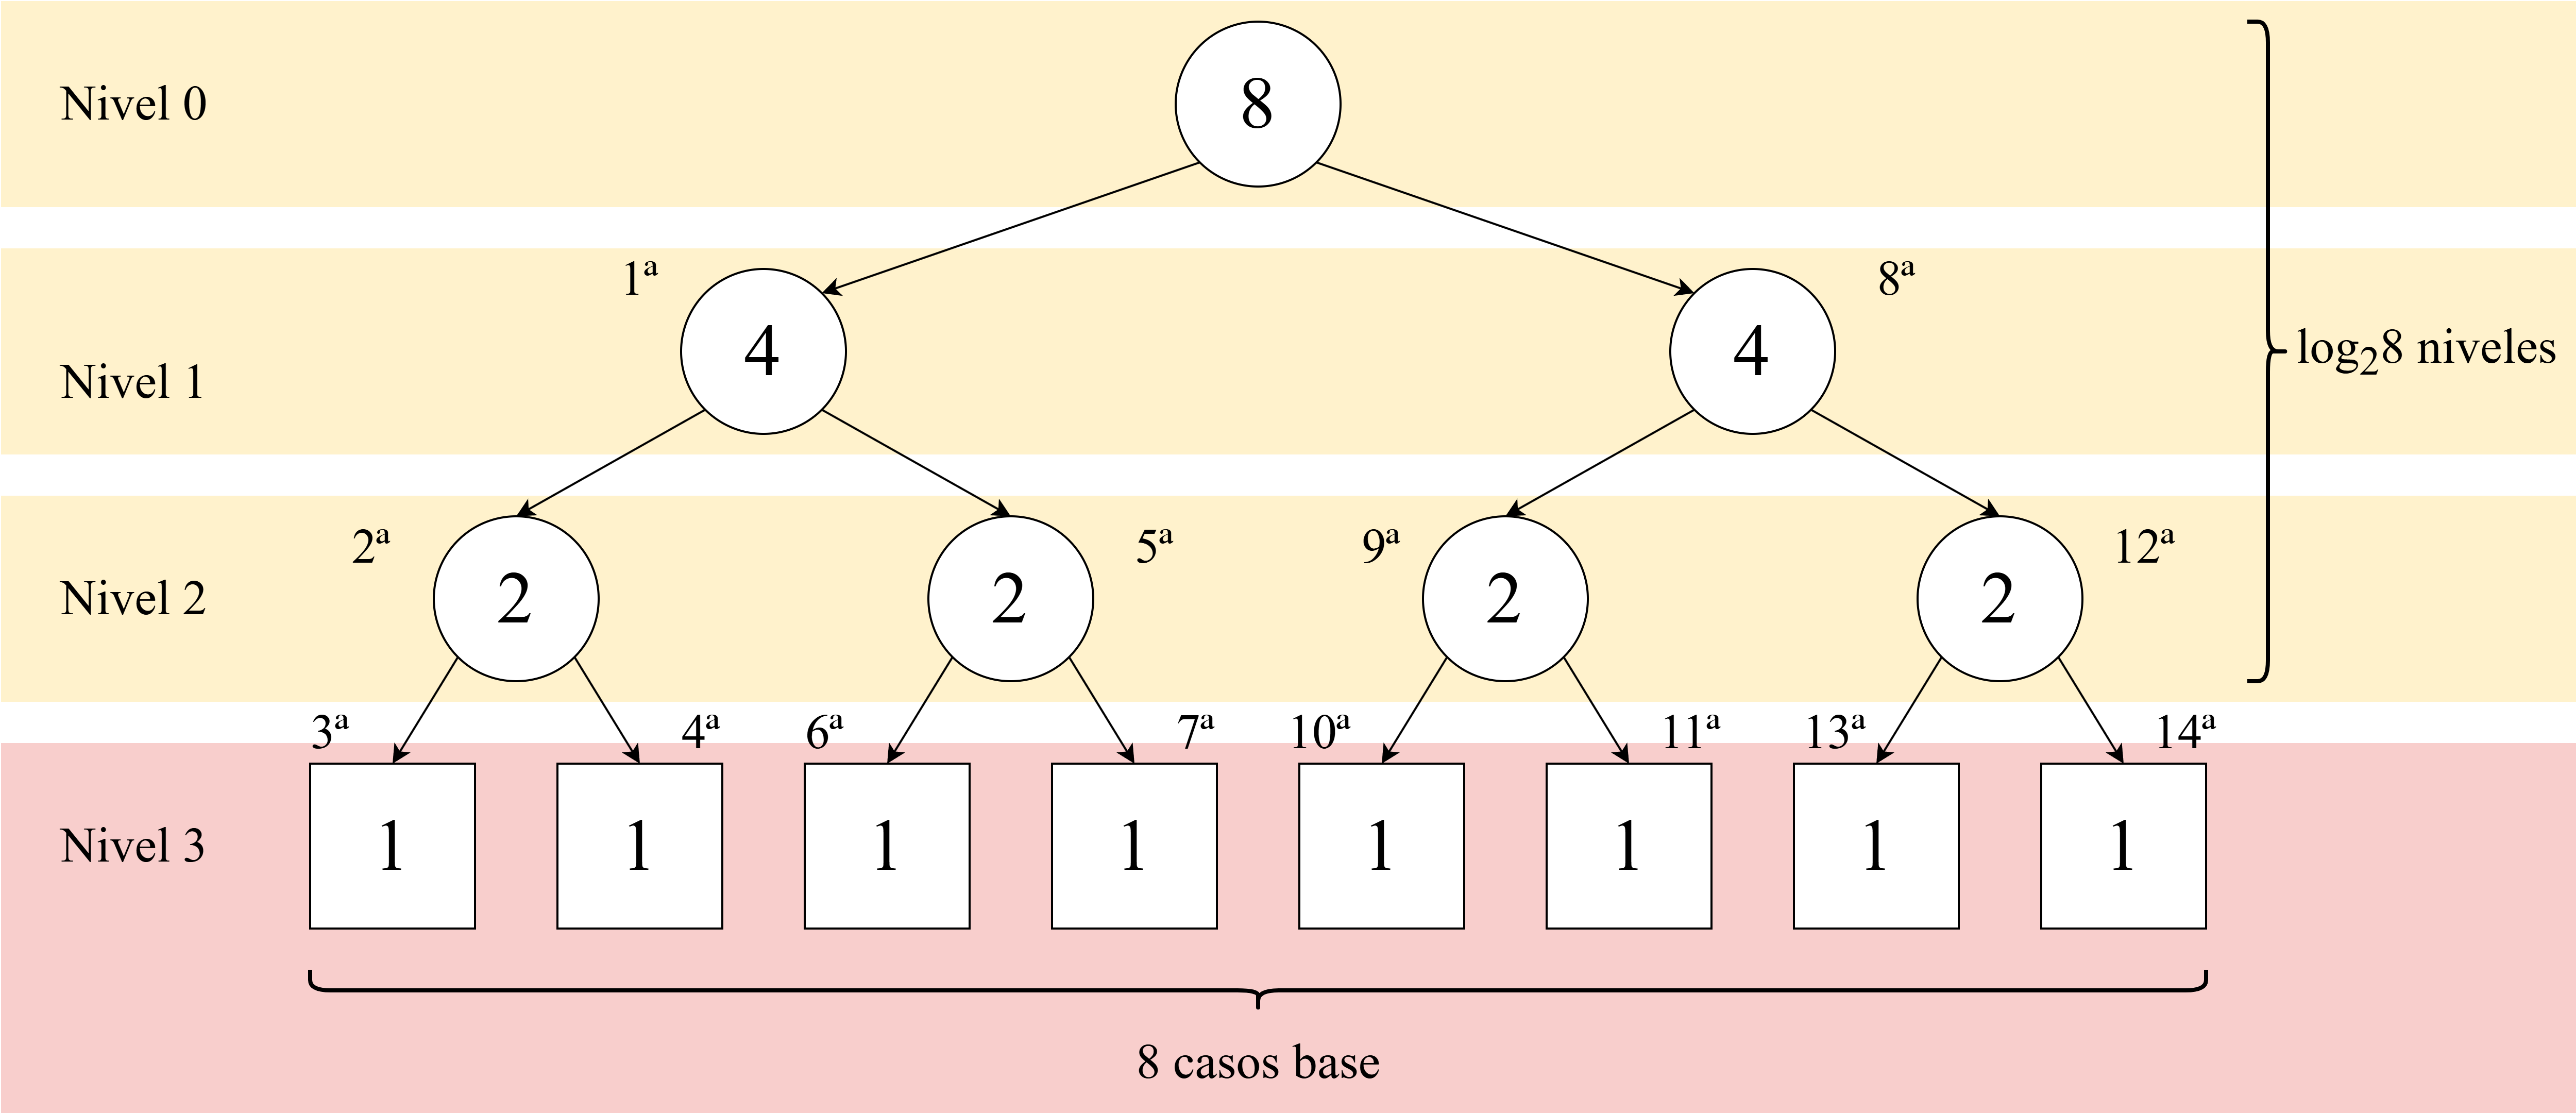
\includegraphics[width=0.8\linewidth]{Diagrames/arbolBinarioMSRSn8.png}
    \caption{Árbol binario para \(n=8\)}
    \label{fig:arbol-MSRS-N=8}
\end{figure}

El anterior cálculo corresponde a una llamada a \lstinline|sort()|, pero esta función es recursiva, por tanto, hay que determinar cuantas veces se llama a \lstinline|sort()| en función del tamaño de la entrada \(n\). Estos se facilita si rastreamos las llamadas a \lstinline|sort()|, por ejemplo mediante un árbol binario como el de la Figura \ref{fig:arbol-MSRS-N=8} donde cada nodo representa la longitud de la entrada \lstinline|lenght|. Se observa que para 8 llamadas hay tres niveles en el árbol, la relación entre 8 y 3 es \(log_{2}{8} = 3\) ya que \(8=2^3\). Por extensión, para un \(n\) tamaño de entrada hay \(\log_{2}{n}\) niveles. Esto se cumple siempre que \(n\) sea múltiplo de 2, lo que da lugar a un árbol balanceado como el de Figura \ref{fig:simetriaMSRS}, en caso contrario está desbalanceado y hay llamadas extras. El trabajo realizado en cada nivel \(i\) es \(2^i\cdot \frac{n}{2^i} = n\) como se observa en la Figura \ref{fig:entradaMSRS} donde \(n\) es el tamaño de entrada original. Finalmente, el trabajo \(f(n)\) de una llamada a \lstinline|sort()| es la suma del trabajo en cada nivel, menos el del último nivel porque los casos bases requieren \(O(1)\) al realizarse un \lstinline|return|; quedando:
\[
	f(n) = \mathlarger{\sum}_{i=0}^{\log_{2}{n} -1} {n} = n\mathlarger{\sum}_{i=0}^{log_{2}{n} -1} {1} = n\cdot\log_{2}{n}
\]

A continuación se aplica la definición de la notación \textit{Big-0} para \(f(n)=n\log_{2}{n}\) y \(g(n)=n\log{n}\). Existe un \(f(n)=O(n\log{n})\) siempre que: 
\[n\log_{2}{n} \leq c\cdot n\log{n}\]
Aislamos la constante \(c\):
\[
	n\log_{2}{n} \leq c\cdot n\log{n} \longrightarrow c \geq \frac{\log_{2}{n}} {\log_{10}{n}} \longrightarrow c \geq \frac{ \frac{\log_{10}{n}} {\log_{10}{2}} } {\log_{10}{n}} \longrightarrow c \geq \frac{1}{\log{2}} 
\]
Esto significa que la complejidad del MSRS se aleja de \(O(n\log{n})\) en un factor aproximado de \(3,32\%\) siempre que la entrada sea mayor que 1 y sea múltiplo de 2. Aun así, la literatura considera que el \textit{Merge Sort} tiene complejidad \(O(n\log{n})\) por razones prácticas. \footnote{\cite{Sedgewick2003-cd}}

\begin{figure}[h]
\centering 
\captionsetup{justification=centering, margin=10pt}
\begin{minipage}{0.5\textwidth} 
    \centering 
    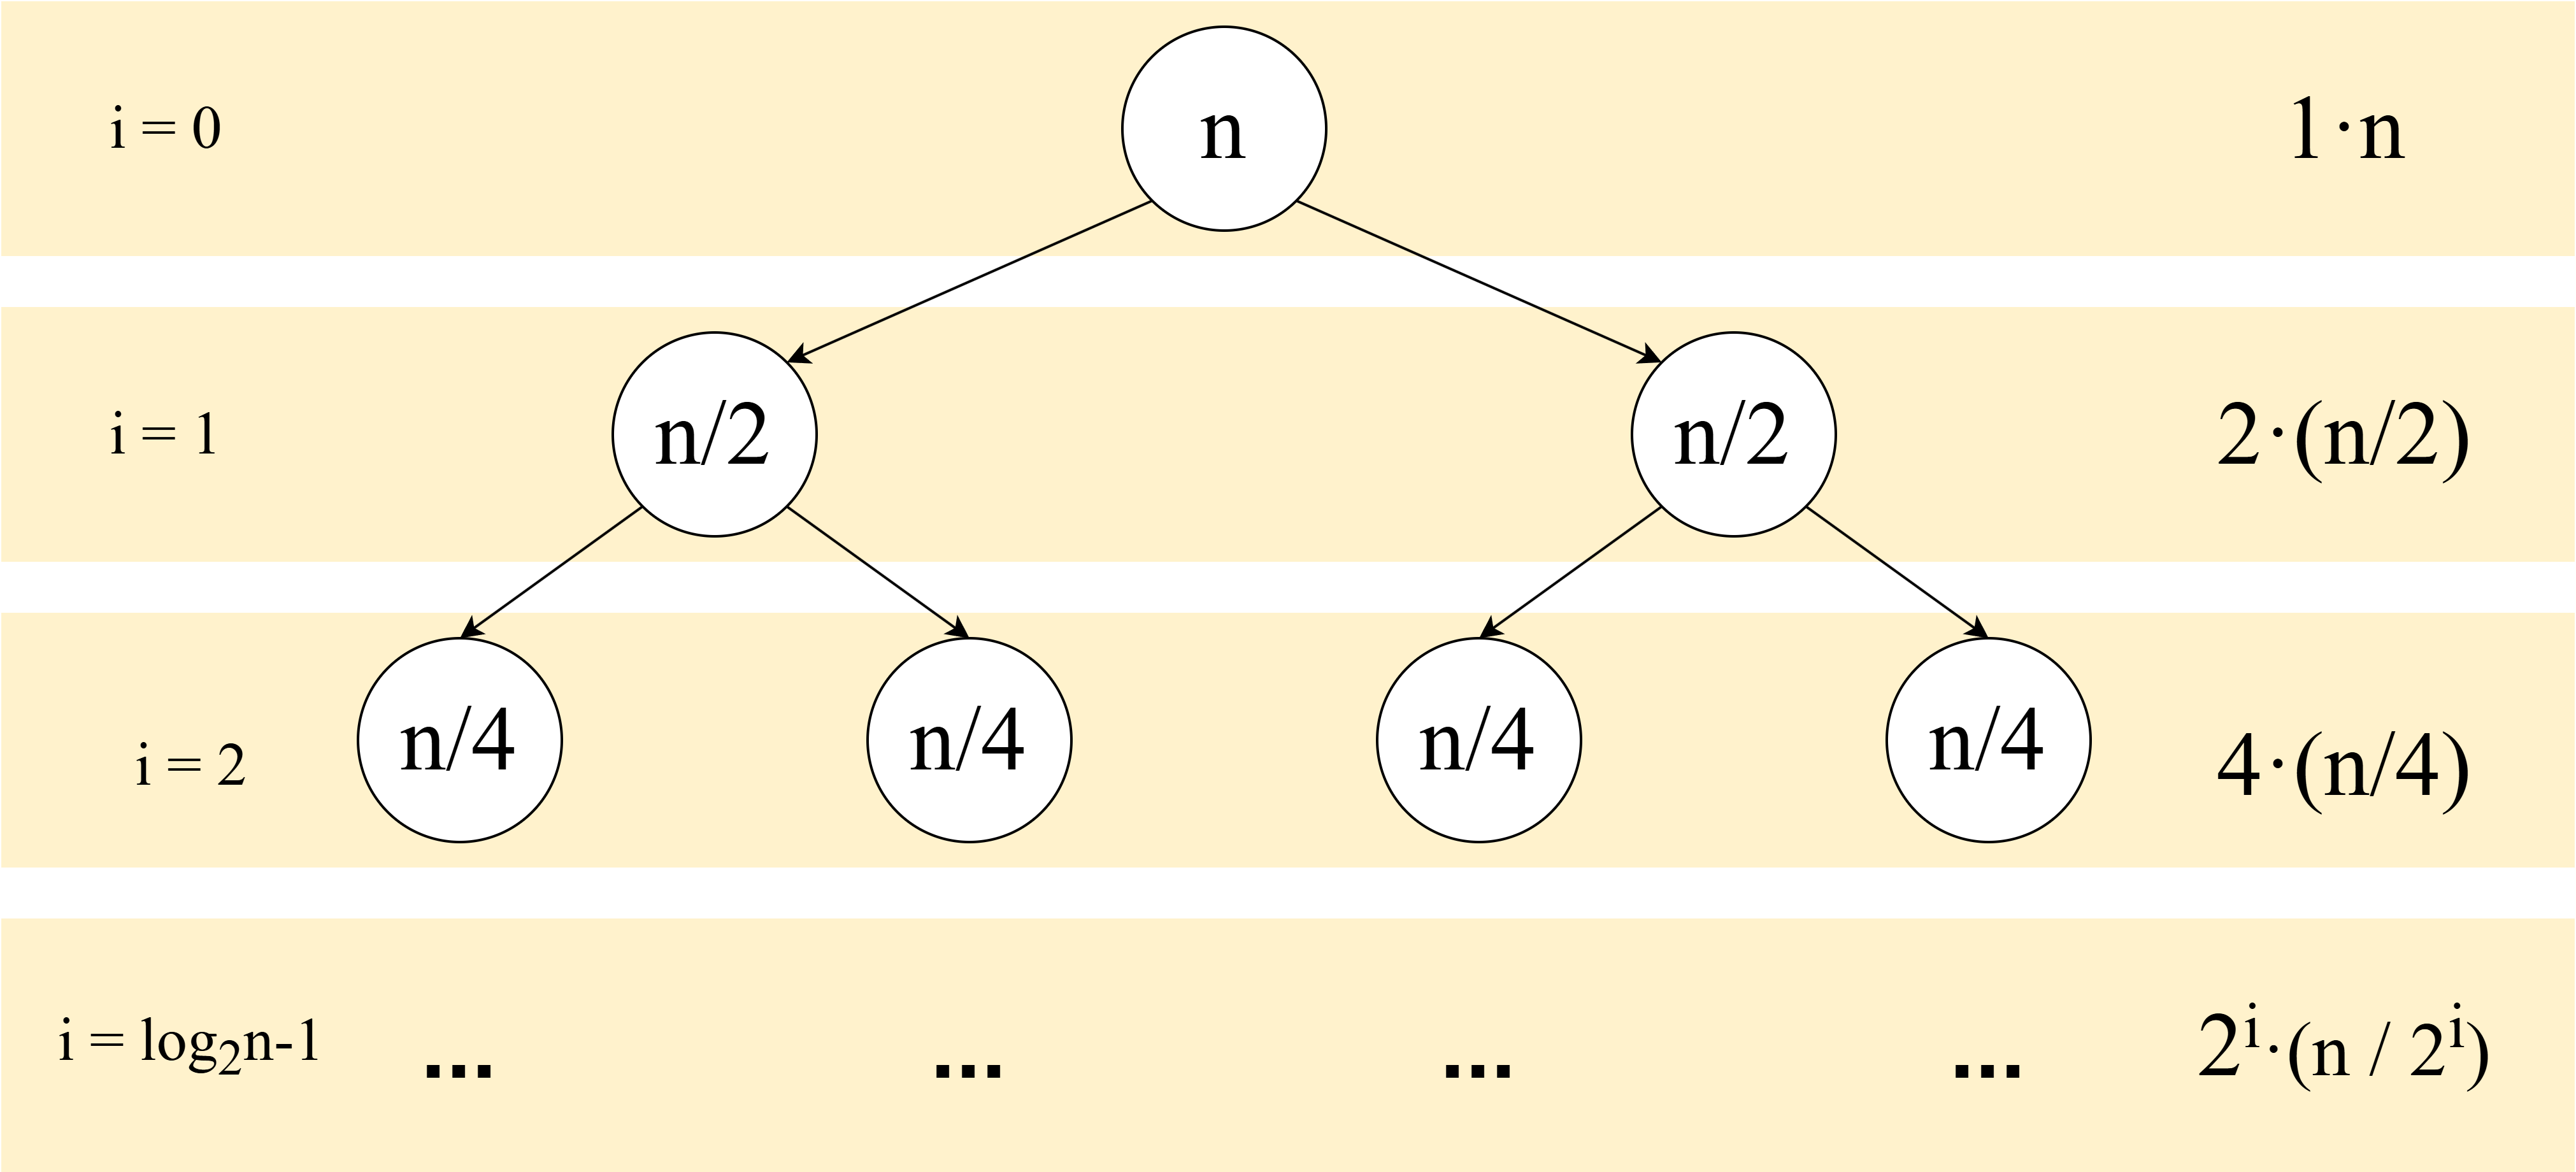
\includegraphics[width=0.95\linewidth]{Diagrames/arbolBinarioLenght.png} 
    \caption{Tamaño de la entrada a lo largo de las llamadas a \lstinline{sort()}} 
    \label{fig:entradaMSRS}
\end{minipage}\hfill 
\begin{minipage}{0.5\textwidth} 
    \centering 
    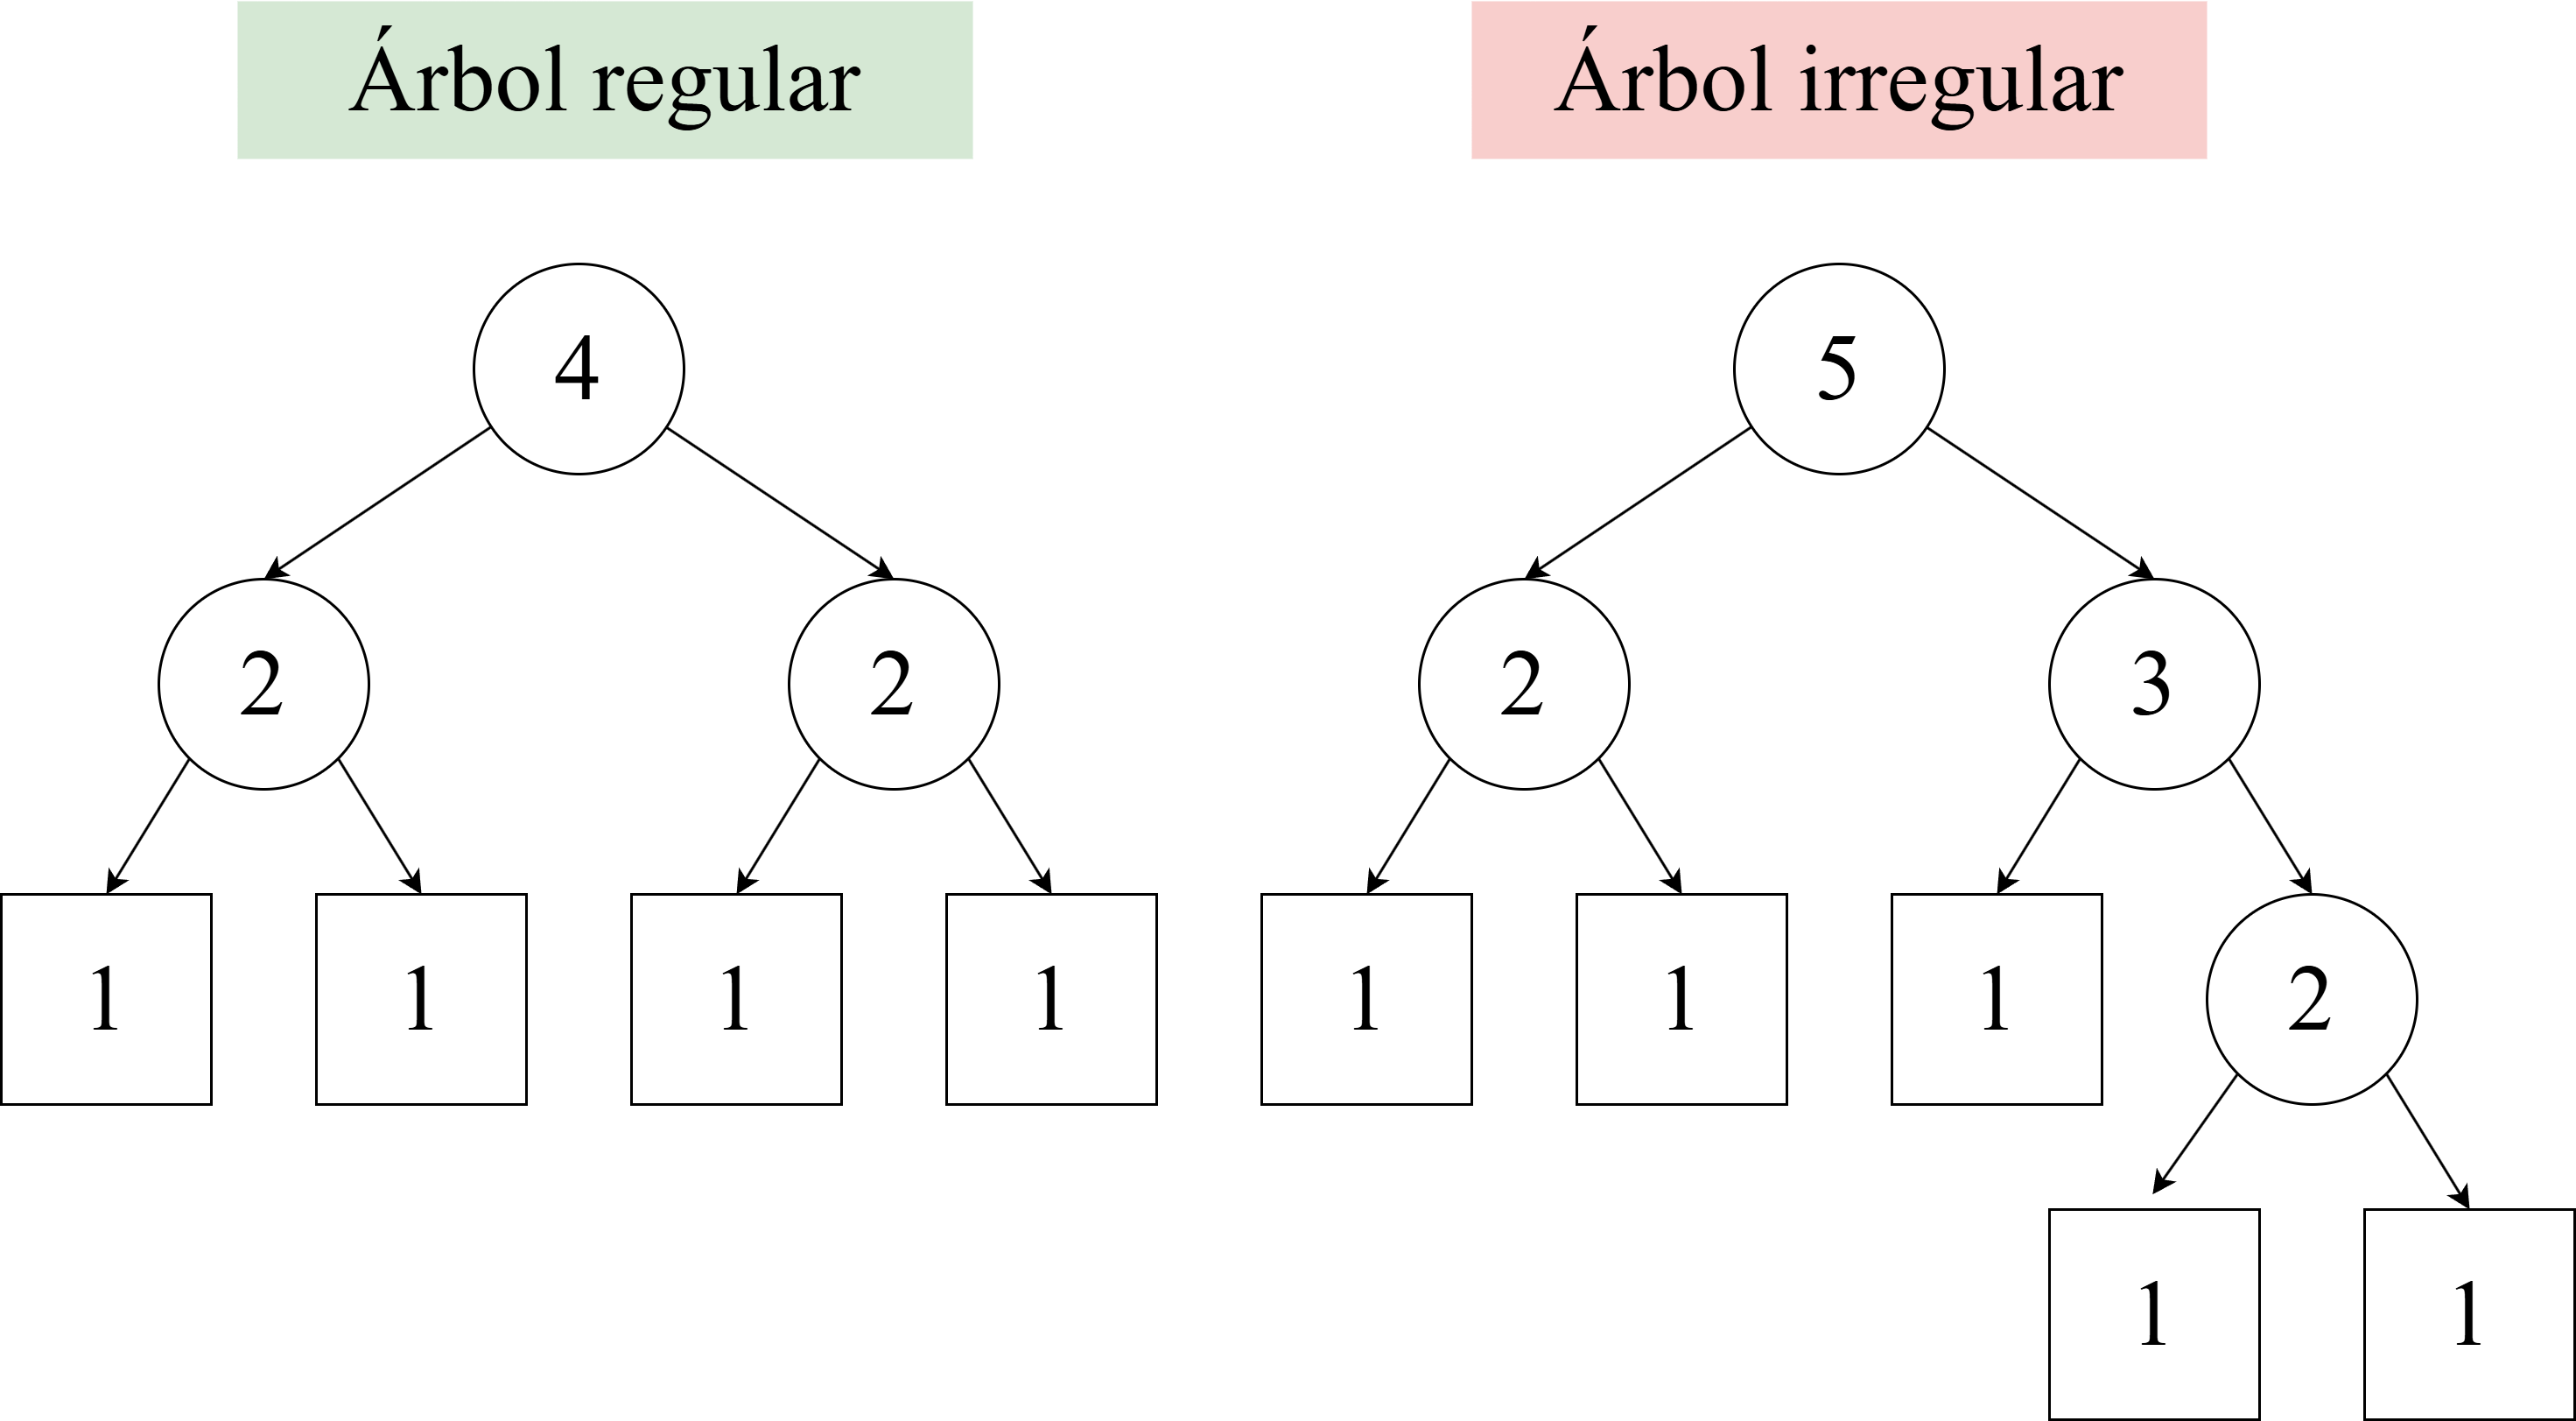
\includegraphics[width=0.95\linewidth]{Diagrames/arbolBinario_MSRS.png} 
    \caption{Árbol balanceado versus árbol desbalanceado del MSRS} 
    \label{fig:simetriaMSRS}
\end{minipage} 
\end{figure}


\subsection{Merge Sort Iterativo Serial (MSIS)} %%142 +6 

El MSIS es la versión análoga al clásico MSRS, en esta implementación se divide la colección en partes más pequeñas, después las partes adyacentes se unen, y se aumenta el tamaño  de las partes. Estos tres pasos se repiten hasta que la parte tenga el tamaño de la colección original. El primer bucle determina el tamaño de las subcolecciones: \lstinline|size| \(=2, 4, 8..\). El segundo bucle recorre \lstinline|arr[]| en pasos de \lstinline|2*size|, uniendo el subarreglo \lstinline|arr[left]..arr[left+size-1]| a su adyacente \lstinline|arr[mid]...arr[right]| mediante \lstinline|merge()|. El índice \lsc{mid} determina el final del primer arreglo y \lstinline|right| el final del adyacente. En la Figura \ref{fig:ejecuciónMSIS} se presenta el proceso de ordenación de una colección de ejemplo: cada nivel es una iteración del segundo bucle donde se une una parte (casillas azules) a su adyacente (casillas amarillas).

\begin{figure}[hbtp]
    \begin{lstlisting}[language=java, frame=single, numbers=left]
public static void sort(int[] arr, int[] aux) {
	int n = arr.length;
	
	for (int size = 1; size < n; size *= 2) {
		for (int left = 0; left < n - size; left += 2 * size) {
			int mid = left + size - 1;
			int right = Math.min(left + 2 * size - 1, n - 1);
			merge(arr, aux, left, mid, right);
		}
	}
}
    \end{lstlisting}
    \caption{Función \lstinline{sort()} del Merge Sort Iterativo Serial}
    \label{fig:MSIS_sort()}
\end{figure}

\subsubsection{Complejidad temporal}%%94 +3
El MSIS recorre el árbol desde la base de la recursión hasta la parte superior, ya que se realizan uniones entre partes de longitud 1-1, 2-2- 4-4... Como en el MSRS, el árbol será balanceado solo si el tamaño de entrada es múltiplo de 2. Siguiendo el mismo método y tomando las mismas suposiciones que en el cálculo de la complejidad temporal del MSRS, la complejidad del MSRS es \(O(n \log{n})\) porque hay \(\log_2{n}-1\) llamadas a \lstinline|sort()| en las cuales se realiza un trabajo de \(O(n)\) en el peor caso.


\begin{figure}[h]
	\centering 
	\captionsetup{justification=centering, margin=10pt}
	\begin{minipage}{0.4\textwidth} 
		\centering
		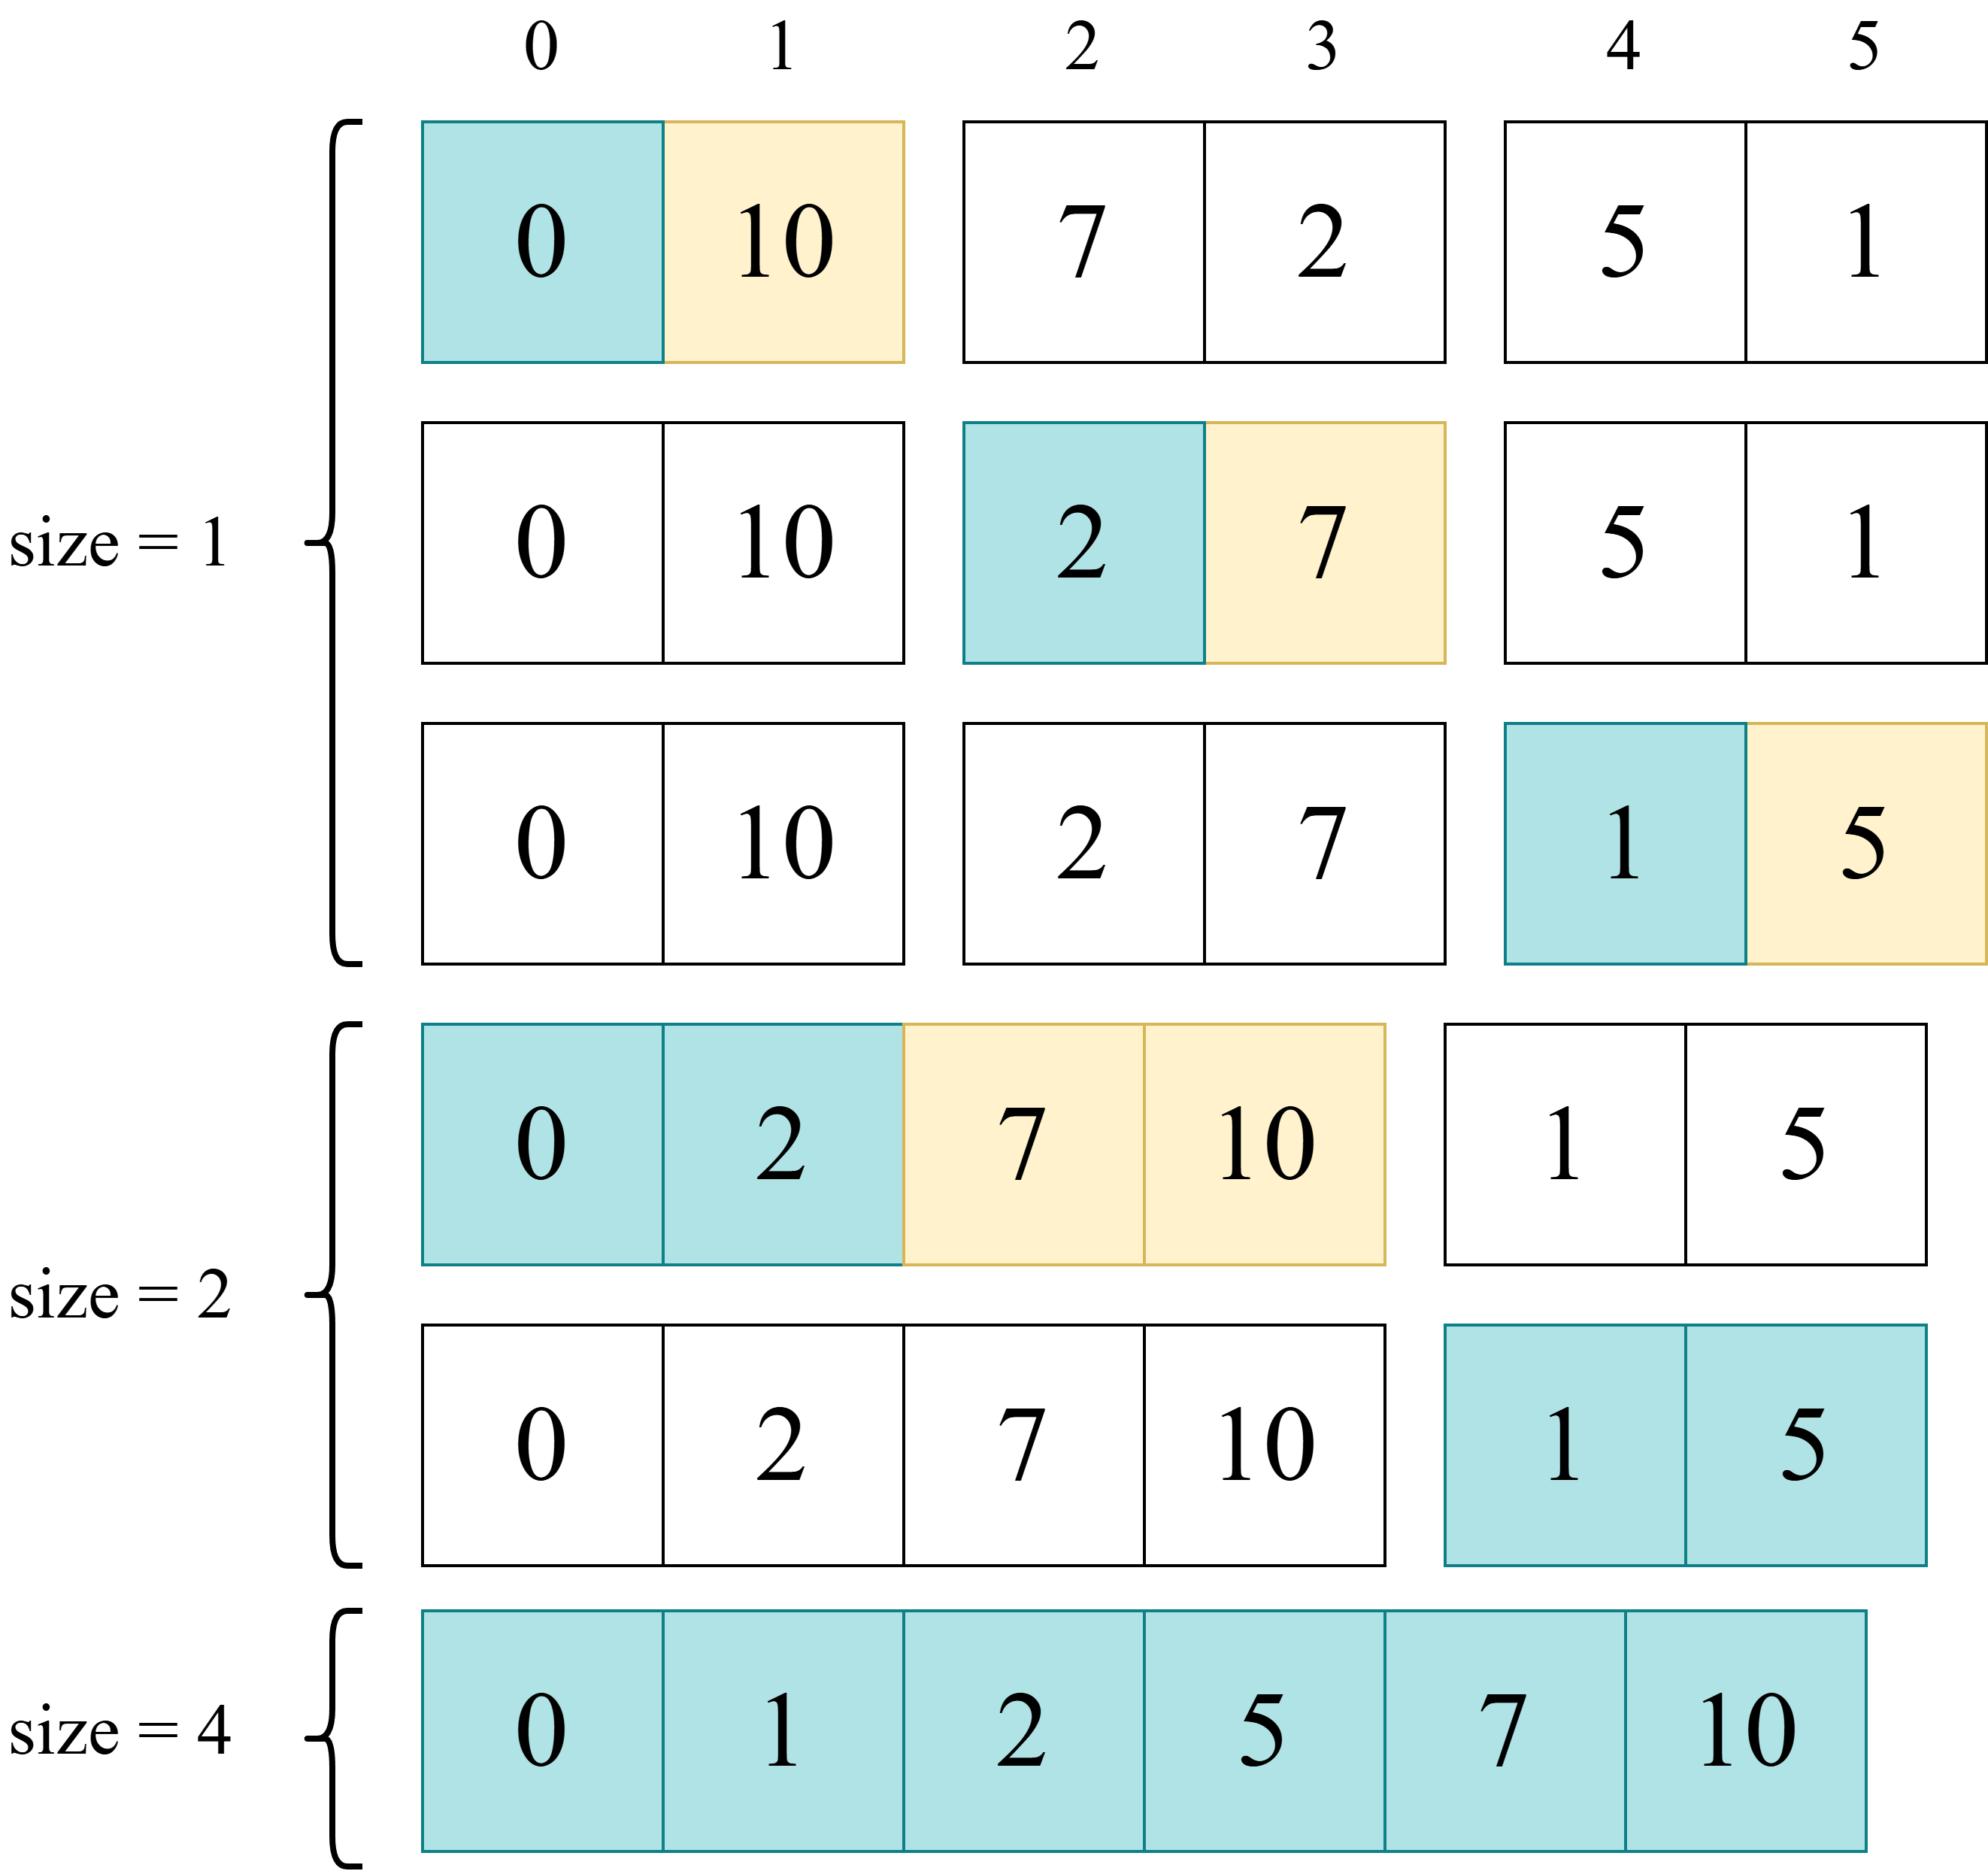
\includegraphics[width=1\linewidth]{Diagrames/ejecucionMSIS.png}
		\caption{Ejecución del Merge Sort Iterativo Serial}
		\label{fig:ejecuciónMSIS}
	\end{minipage}\hfill \hspace{3pt}
	\begin{minipage}{0.55\textwidth} 
		\centering
		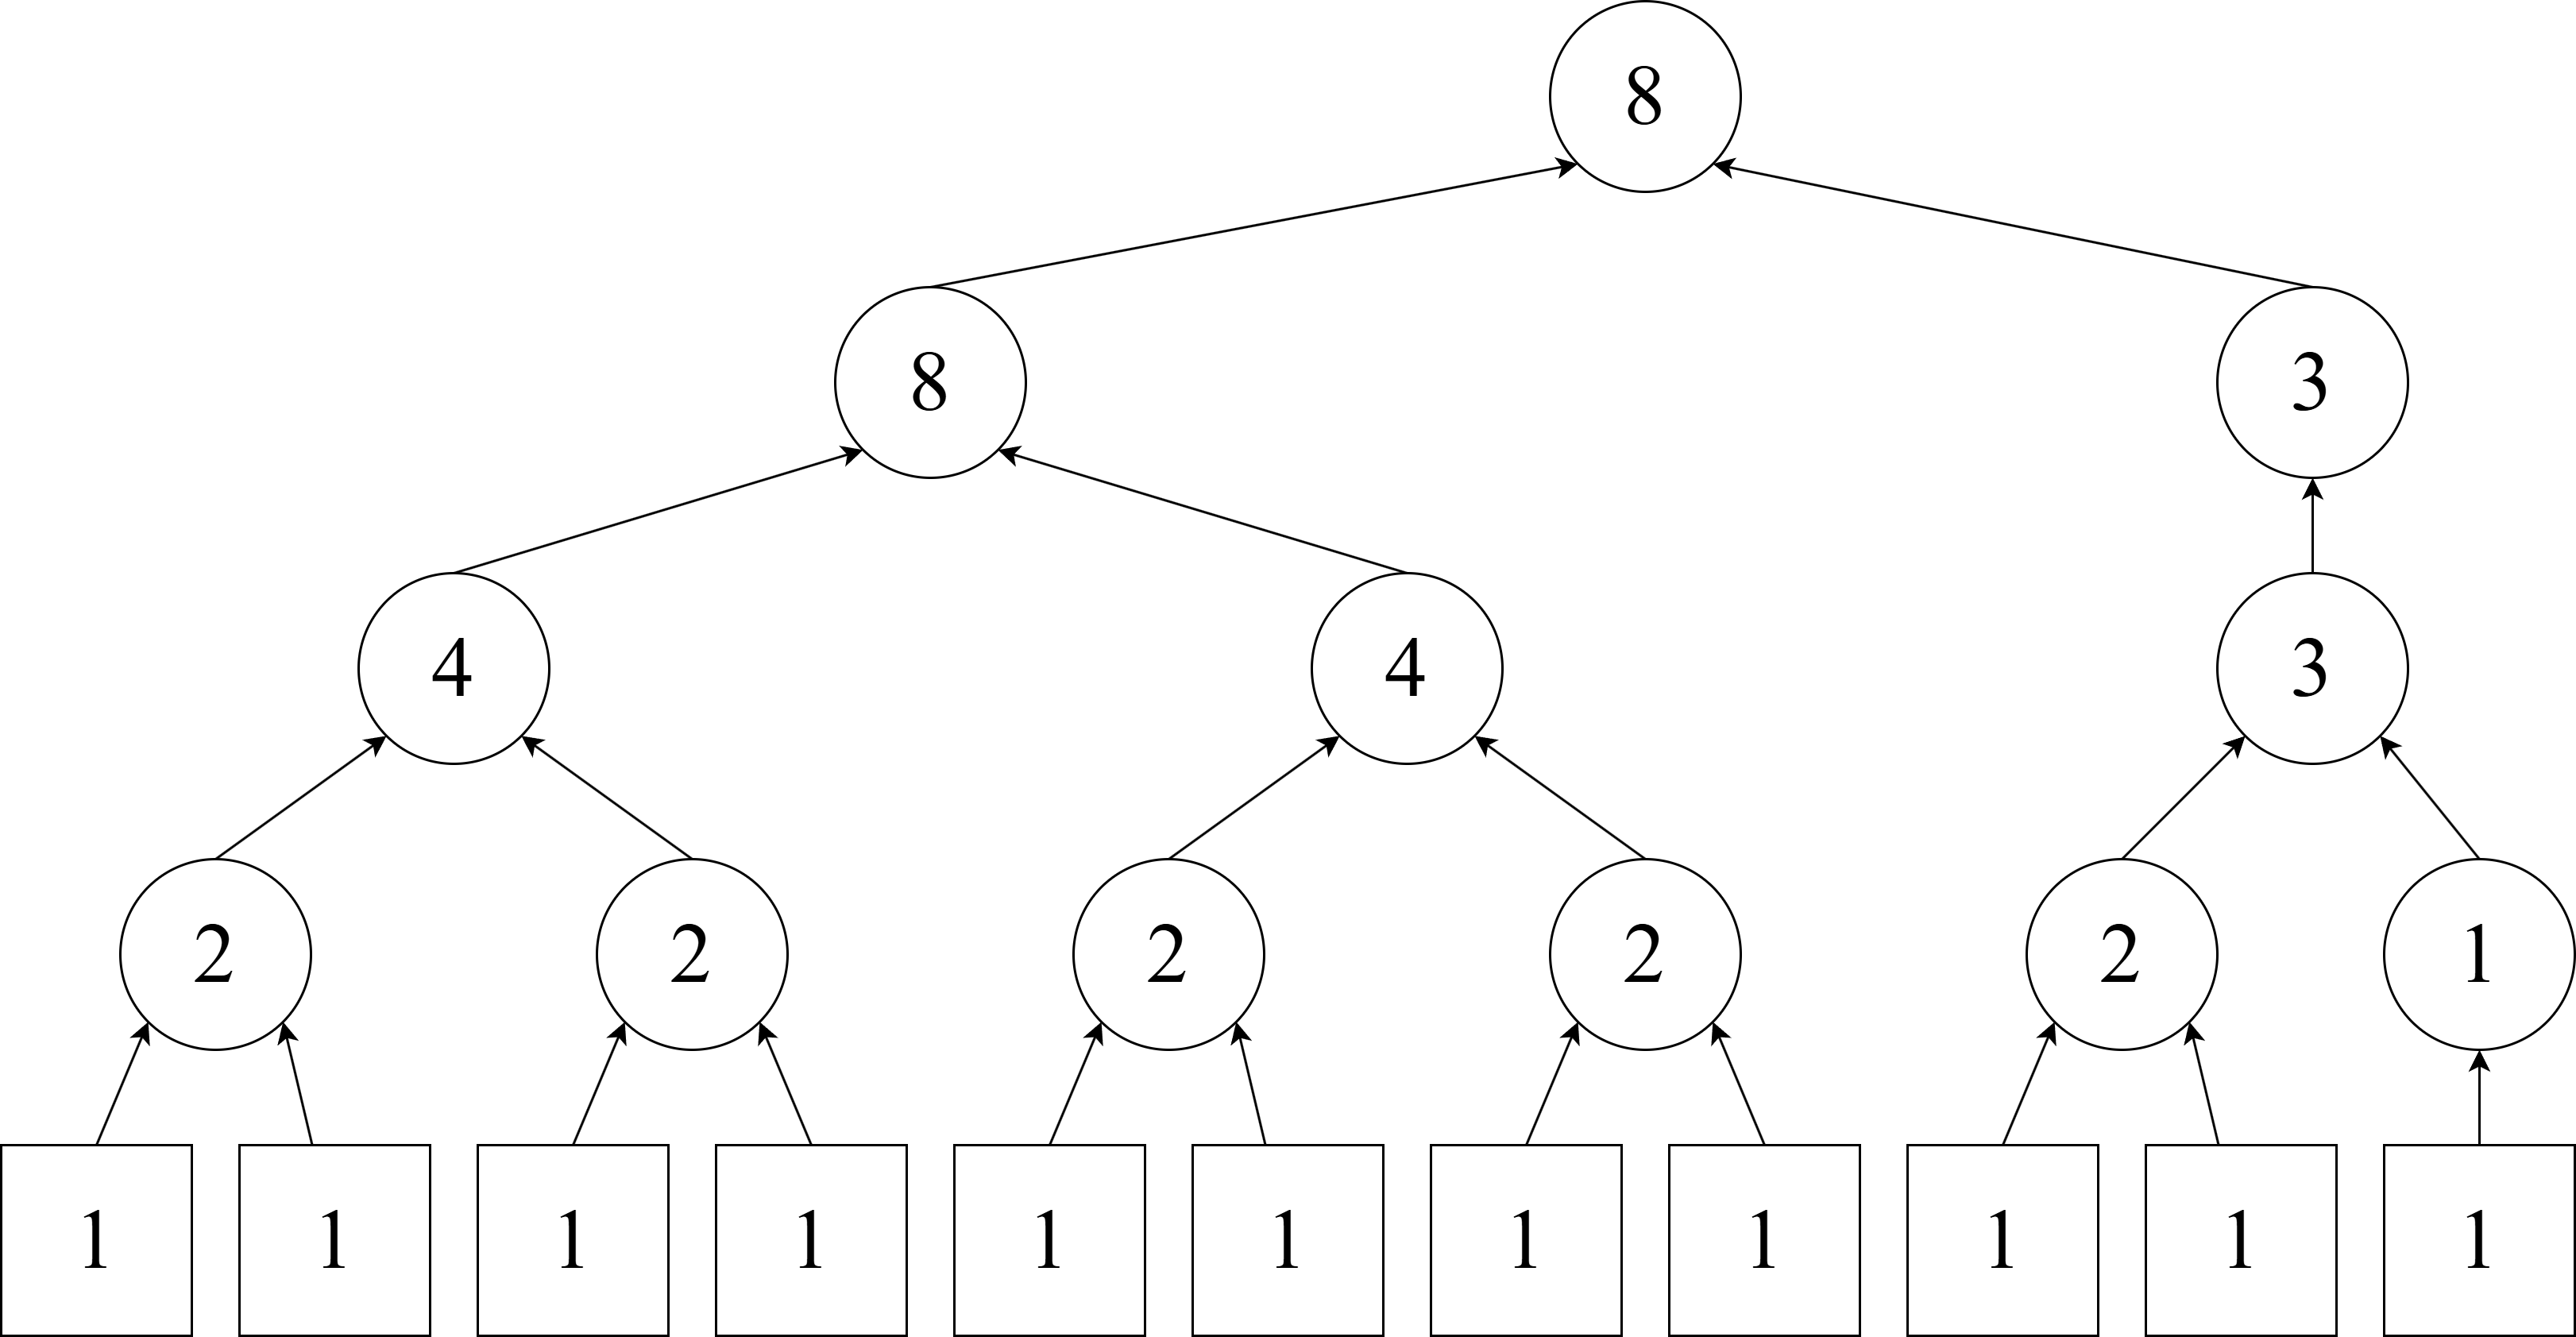
\includegraphics[width=1\linewidth]{Diagrames/arbolMSISirregular.png}
		\caption{Árbol binario del Merge Sort Iterativo Serial}
		\label{fig:arbolMSIS}
	\end{minipage} 
\end{figure}

\newpage
%%753
\subsection{Merge Sort Recursivo Paralelo (MSRP)}%%670 +6 %%VOLVER A CONTAR
Un \textbf{proceso} es la ejecución de las instrucciones de un programa; después de que estas instrucciones se hayan movido desde la memoria secundaria hasta la primaria. El sistema operativo crea los procesos y guarda en la memoria información asociada. En cambio, un \textbf{hilo de ejecución} es una secuencia de instrucciones que el planificador del sistema operativo puede manejar independientemente. \footnote{\cite{bobrov-2023}} Hasta el momento se han mostrado programas que al ejecutarse toman la forma de un proceso con un solo hilo de ejecución (MSIS y MSRS). La idea es mejorar el rendimiento del \textit{Merge Sort} haciendo uso de más de un hilo de ejecución. 

La herramienta más apropiada que proporciona Java para este problema es la clase \lstinline|ForkJoinPool|.\footnotemark \footnotetext{\cite{OracleForkJoin}} Una piscina de hilos es un espacio en el que se mantienen un conjunto fijo de hilos de ejecución reusables que esperan a que se les pase un conjunto de instrucciones a ejecutar. Una piscina evita la necesidad de crear y destruir hilos constantemente, hecho que conlleva un costo computacional elevado.\footnote{\cite{engle_2022}}

\begin{figure}[h]
	\centering
	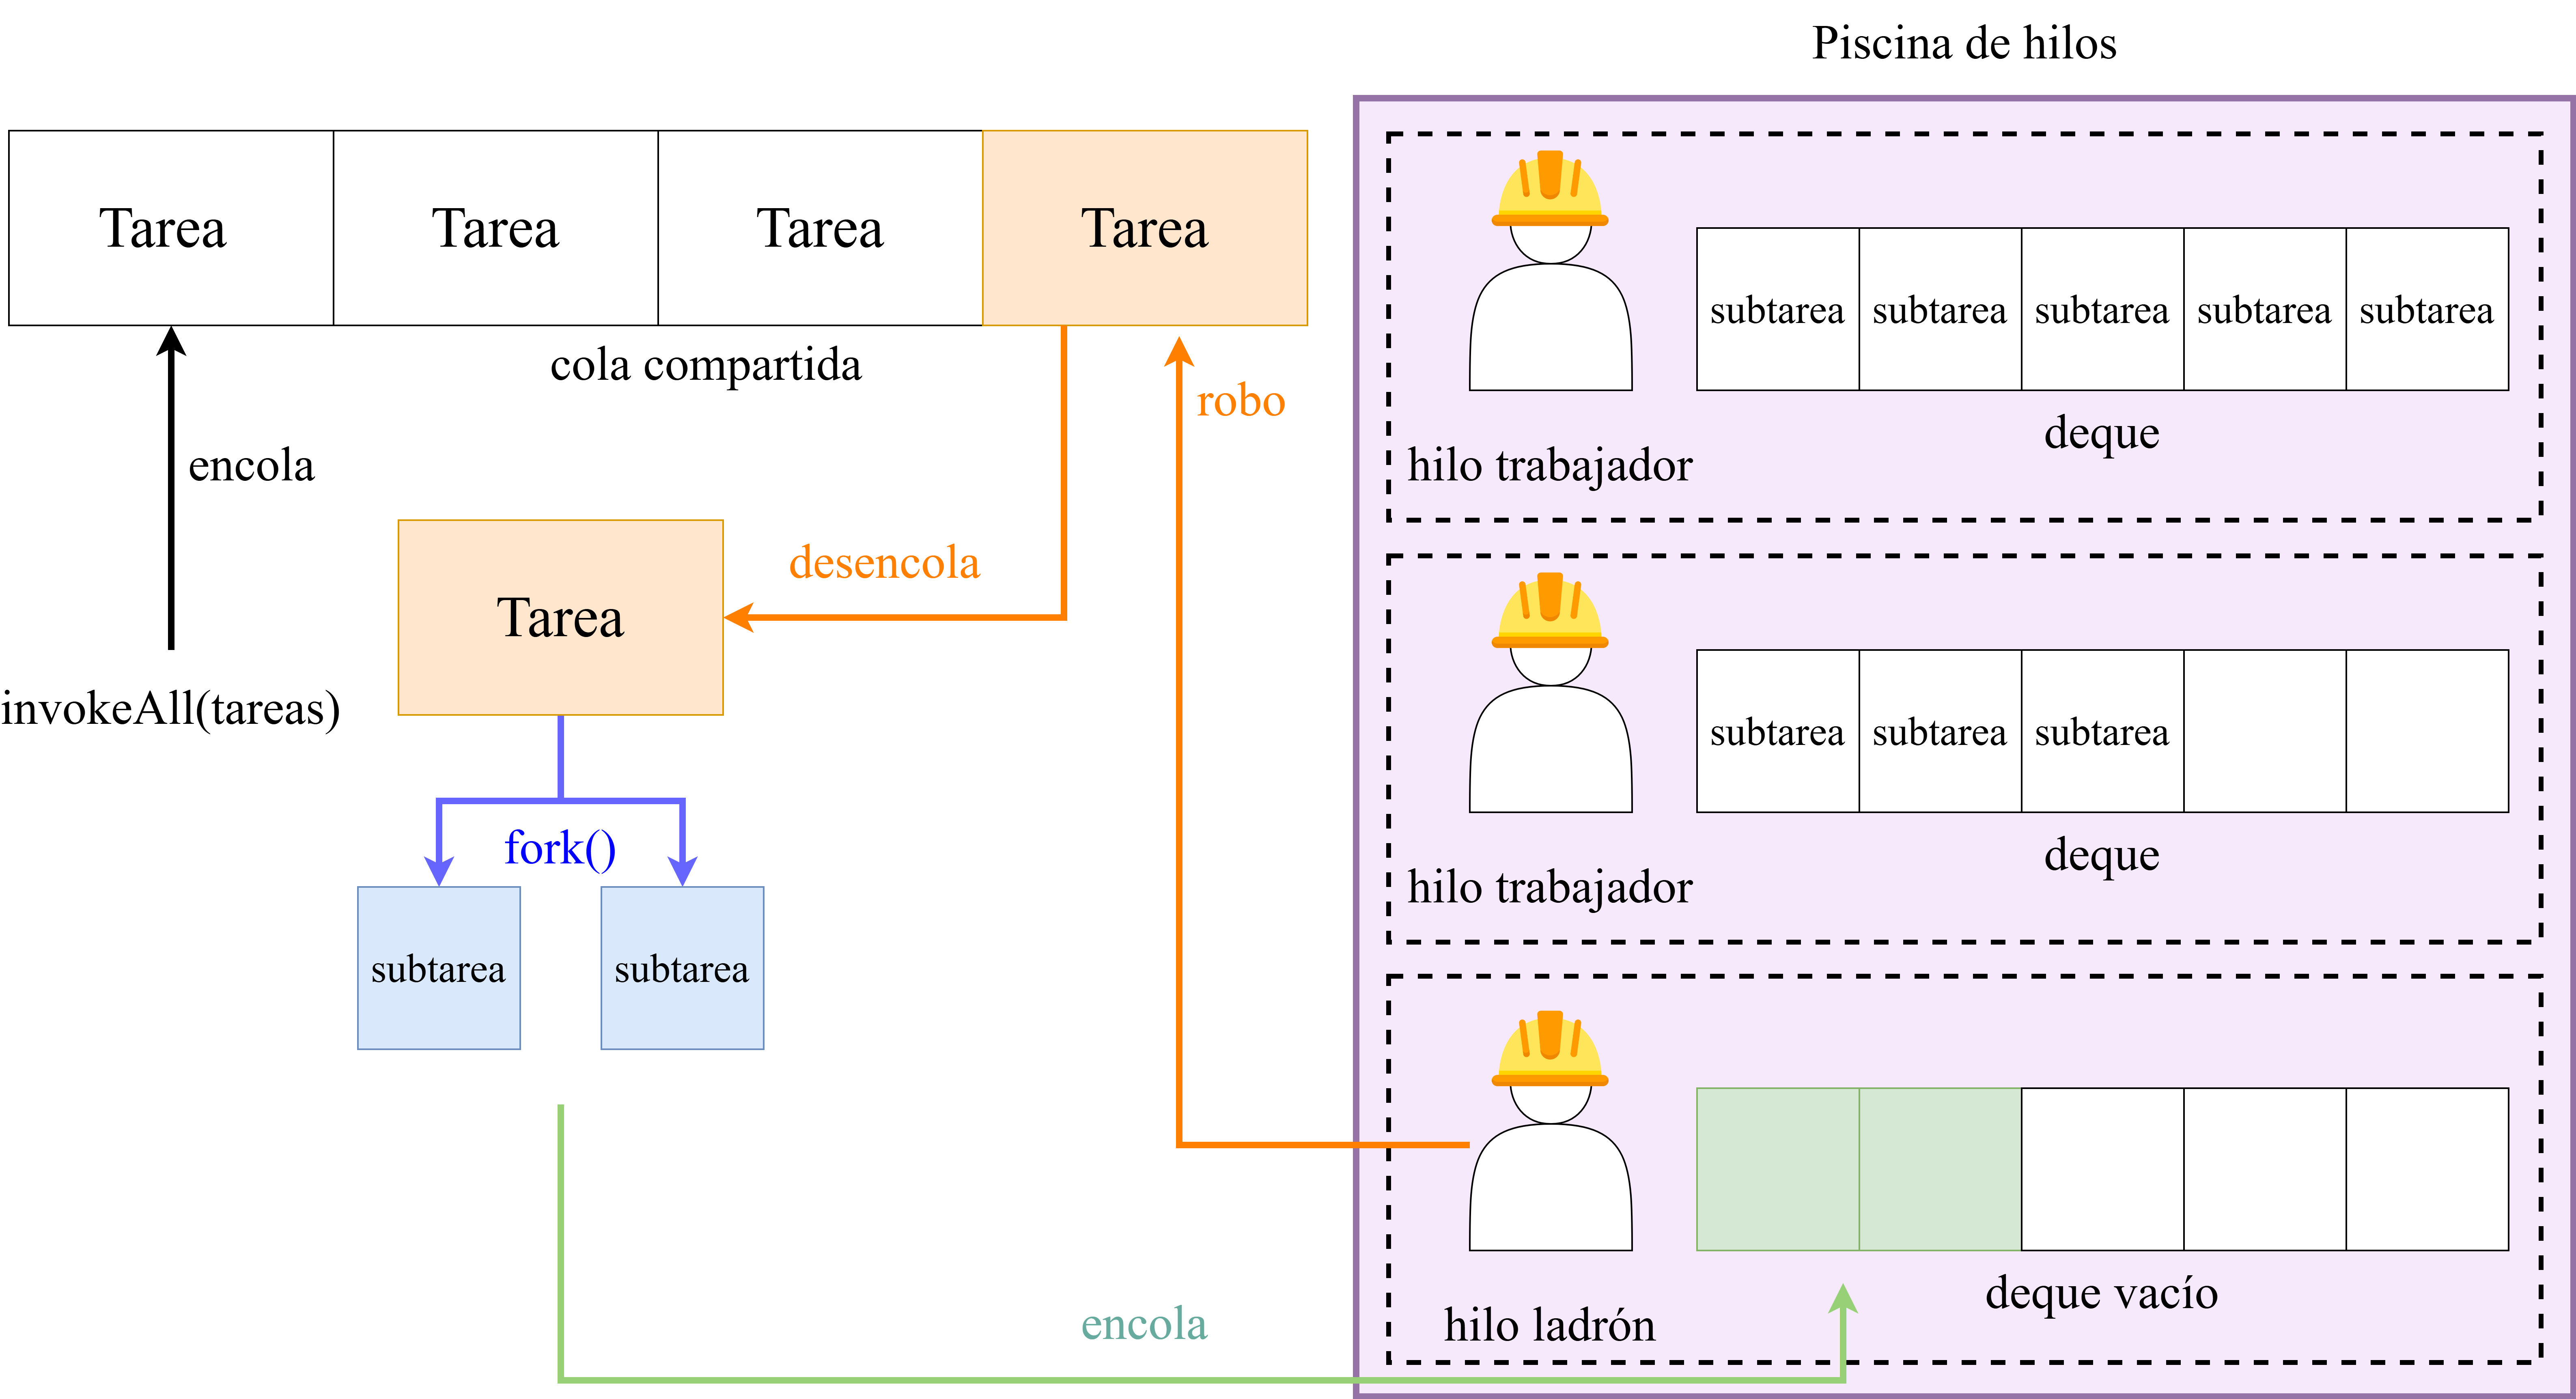
\includegraphics[width=0.75\linewidth]{Diagrames/forkJoinPool.png}
	\caption{Funcionamiento del \lstinline{ForkJoinPool}}
	\label{fig:forkJoinPool}
\end{figure}

La \lstinline|ForkJoinPool| permite crear piscinas basadas en un algoritmo de robo de trabajo (\textit{work-stealing}).\footnote{\cite{Ramgir2017-mv}} Esto significa que las tareas se acumulan en una cola compartida entre todos los hilos, pero, además, cada hilo consta de su propia cola doblemente terminada (decola). Los hilos extraen de la cola las tareas y las ejecutan, si la tarea produce subtareas estas se guardan en su decola. Puede ocurrir que la decola de un hilo se vacíe, en ese caso, el hilo desencola una tarea de la cola compartida.\footnote{\cite{kumar_2024}} La \lstinline|ForkJoinPool| es útil si el algoritmo genera muchas subtareas, ya que el uso de decolas propias reduce significativamente la cantidad de accesos a la cola compartida.\footnote{\cite{blumofe1999scheduling}} Adicionalmente, las tareas de la cola compartida serán siempre de mayor tamaño que las subtareas que generen tareas ubicadas en las decolas. Por ende, \lstinline|ForkJoinPool| es apropiada para la paralelización del \textit{Merge Sort}, en tanto que se generan subtareas que después se volverán a unir.

\begin{figure}[h]
	\begin{lstlisting}[language=java, frame=single, numbers=left]
ForkJoinPool pool = new ForkJoinPool(parallelismLevel);
MSrecursivoParalelo task = new MSrecursivoParalelo(arr, aux, left, right);
pool.invoke(task);
	\end{lstlisting}
	\caption{Inicialización de la \lstinline{ForkJoinPool}}
	\label{fig:creacionForkJoinPool}
\end{figure}

Para crear una \lstinline|ForkJoinPool| se llama a su constructor y se pasa el número de hilos trabajadores que tendrá la piscina (\lstinline|parallelismLevel|). Después, se debe pasar una tarea a la piscina que esta procesará cuando se llame al método \lstinline|.invoke()|. Existen dos tipos tareas: aquellas que no retornan ningún valor (\lstinline|RecursiveAction|) y aquellas que sí retornan (\lstinline|RecursiveTask|).\footnote{\cite{jenkov2024forkjoinpool}} En este caso, se pasa una tarea del tipo \lstinline|RecursiveAction|. (Figura \ref{fig:creacionForkJoinPool})

Concretamente, la lógica del MSRP se inscribe en una clase \lstinline|MSrecursivoParalelo| que hereda de la clase abstracta \lstinline|RecursiveAction| (Figura \ref{fig:MSRP_RecursiveAction}). 

\begin{figure}[h]
	\begin{lstlisting}[language=java, frame=single, numbers=left]
public class MSrecursivoParaleloSinUmbral extends RecursiveAction {
	private final int[] arr, aux;
	private final int right, left;
	
	public MSrecursivoParaleloSinUmbral(int[] arr, int[] aux, int left, int right) {
		this.arr = arr;
		this.aux = aux;
		
		this.left = left;
		this.right = right;
	}
	
	@Override
	protected void compute() {	}
	
	private static void merge(int[] arr, int[] aux, int left, int mid, int right) {	}	
}    	
	\end{lstlisting}
	\caption{Esquema de la clase \lstinline{MergeSortRecursivoParalelo}}
	\label{fig:MSRP_RecursiveAction}
\end{figure}

En dicha clase el algoritmo queda encapsulado en el método  \lstinline|compute()|, como se observa en la Figura \ref{fig:MSRP_Compute}. Primero se comprueba el caso base. Después se crean dos subtareas, por ahora inactivas, para cada lado de la colección. A continuación, se pasan las subtareas a \lstinline|invokeAll()|, que las encola en la cola compartida de piscina y espera a que \lstinline|Left| y \lstinline|Right| finalicen. Finalmente, se unen las dos partes con el mismo algoritmo común \lstinline|merge()|.

\begin{figure}[h]
    \begin{lstlisting}[language=java, frame=single, numbers=left]
@Override
protected void compute() {
	if (left >= right) return;
	
	int mid = left + (right - left) / 2;
	
	final MSrecursivoParalelo Left = new MSrecursivoParalelo(arr, aux, left, mid);
	final MSrecursivoParalelo Right = new MSrecursivoParalelo(arr, aux, mid + 1, right);
	
	invokeAll(Left, Right);
	
	merge(arr, aux, left, mid, right);
}
    \end{lstlisting}
    \caption{Método \lstinline{compute()} del MSRP}
    \label{fig:MSRP_Compute}
\end{figure}

Normalmente llega un momento en que generar más subtareas torna ineficiente dado que el costo de gestión de hilos es mayor que el costo que conllevaría ejecutar las tareas de forma serial. En este caso, colecciones con baja longitud ralentizarían al MSRP. Por ende es común establecer un umbral (\textit{threshold}) a partir del cual se ejecutan las subtareas serialmente.

\begin{figure}[h]
	\begin{lstlisting}[language=java, frame=single, numbers=left]
protected void compute() {
	int length = (right + 1 - left);
	if (length <= THRESHOLD) {
		MSrecursivoSerial.sort(arr, aux, left, right);
	} else {
		// Ejecucion paralela
	}
}
	\end{lstlisting}
	\caption{MSRP modificado con umbral}
	\label{fig:computeModificado}
\end{figure}

Se ha conducido un test piloto para determinar el umbral adecuado para esta implementación. Se han tomado 50 muestras del tiempo de ejecución para 20 longitudes de arreglo para el MSRS y para el MSRP, pero sin un umbral definido (Figura \ref{fig:MSRP_Compute}). En la Tabla \ref{tab:testPilotoMSRP} se comparan los promedios de las muestras obtenidas. Los tamaños de las colecciones son potencias de dos, en tanto que se intenta conseguir un árbol binario balanceado que aprovecha mejor los recursos. Obsérvese que hasta el tamaño $2^{15}$ el algoritmo más rápido es el MSRS. Entonces se modifica el método \lstinline|compute()| para que, en caso de que la longitud del arreglo de entrada sea inferior al umbral de $2^{15}$, se ejecute la versión serial. (Figura \ref{fig:computeModificado})

\begin{figure}
	\centering
	\begin{tikzpicture}
		\centering
		\begin{axis}[
			xlabel={Tamaño de la colección},
			ylabel={Tiempo (ms)},
			legend pos=north west,
			grid=major,
			width=12cm,
			height=8cm,
			xtick={1, 2, 3, 4, 5, 6, 7, 8, 9, 10, 11, 12, 13, 14, 15, 16, 17, 18, 19, 20},
			xticklabels={$$,$2^2$, $$, $2^4$, $$, $2^6$, $$, $2^8$, $$, $2^{10}$, $$, $2^{12}$, $$, $2^{14}$, $$, $2^{16}$, $$, $2^{18}$, $$, $2^{20}$}
			]
			\addplot coordinates {
				(1, 0.002) (2, 0.004) (3, 0.003) (4, 0.003) (5, 0.005) (6, 0.004) (7, 0.005) (8, 0.013) (9, 0.027) (10, 0.057) (11, 0.120) (12, 0.263) (13, 0.529) (14, 1.099) (15, 2.224) (16, 4.603) (17, 9.332) (18, 19.450) (19, 39.380) (20, 81.661)
			};
			\addlegendentry{MSRS}
			
			\addplot coordinates {
				(1, 0.271) (2, 0.325) (3, 0.375) (4, 0.402) (5, 0.519) (6, 0.751) (7, 0.806) (8, 0.924) (9, 0.987) (10, 1.109) (11, 1.227) (12, 1.424) (13, 1.468) (14, 1.689) (15, 2.186) (16, 2.529) (17, 3.770) (18, 6.248) (19, 11.012) (20, 25.592)
			};
			\addlegendentry{MSRP sin umbral}
		\end{axis}
	\end{tikzpicture}
	\caption{Datos de prueba para MSRS y MSRP sin umbral} 
	\label{fig:testPilotoMSRP}
\end{figure}

\definecolor{Alto}{rgb}{0.87,0.87,0.87}
\begin{table}
	\centering
	\begin{tblr}{
			cells = {c},
			cell{1}{1} = {Alto},
			cell{1}{2} = {Alto},
			cell{1}{3} = {Alto},
			vline{1-4} = {-}{},
			hline{-} = {1-3}{},
		}
		Tamaño  & Tiempo MSRS (ms) & Tiempo MSRP sin umbral (ms) &  \\
		2       & 0,002            & 0,271                       &  \\
		4       & 0,004            & 0,325                       &  \\
		8       & 0,003            & 0,375                       &  \\
		16      & 0,003            & 0,402                       &  \\
		32      & 0,005            & 0,519                       &  \\
		64      & 0,004            & 0,751                       &  \\
		128     & 0,005            & 0,806                       &  \\
		256     & 0,013            & 0,924                       &  \\
		512     & 0,027            & 0,987                       &  \\
		1024    & 0,057            & 1,109                       &  \\
		2048    & 0,120            & 1,227                       &  \\
		4096    & 0,263            & 1,424                       &  \\
		8192    & 0,529            & 1,468                       &  \\
		16384   & 1,099            & 1,689                       &  \\
		32768   & 2,224            & 2,186                       &  \\
		65536   & 4,603            & 2,529                       &  \\
		131072  & 9,332            & 3,770                       &  \\
		262144  & 19,450           & 6,248                       &  \\
		524288  & 39,380           & 11,012                      &  \\
		1048576 & 81,661           & 25,592                      &  
	\end{tblr}
	\caption{Datos de prueba para MSRS y MSRP sin umbral} 
	\label{tab:testPilotoMSRP}
\end{table}

\newpage
%%374
\subsection{Merge Sort Iterativo Paralelo (MSIP)} %%376+6
Para la paralelización del algoritmo iterativo se ha hecho uso de la interfaz \lstinline|ExecutorService| que proporciona Java y que proporciona un marco para gestionar y controlar la ejecución de tareas asincrónicas. A diferencia de las piscinas \lstinline|ForkJoin|, el \lstinline|ExecutorService| utiliza un algoritmo de trabajo compartido (\textit{work-sharing algorithm}). Esto implica que solo hay una cola compartida entre todos los hilos: una vez termina un hilo de ejecutar una subtarea, extrae otra de la cola. Este flujo de ejecución es apropiado para tareas independientes entre ellas.\footnote{\cite{OracleExecutorService}}

\begin{figure}[h]
	\centering
	\begin{lstlisting}[language=java, frame=single, numbers=left]
public static void sort(int[] array, int aux[], ExecutorService executor) {
	int length = arr.length;
	List<Future<?>> futures = new ArrayList<>();
	
	for (int size = 1; size < length; size *= 2) {
		
		for (int left = 0; left < length - size; left += 2 * size) {
			int mid = left + size - 1;
			int right = Math.min(left + 2 * size - 1, length - 1);
			int finalLeft = left; //El resto son efectivamente finales
			futures.add(executor.submit(() -> merge(arr, aux, finalLeft, mid, right)));
		}
		for (Future<?> future : futures) {
			try {
				future.get();
			} catch (Exception e) {
				e.printStackTrace();
			}
		}
		futures.clear();
		
	}
	executor.shutdown();
}
	\end{lstlisting}
	
	\caption{Método \lstinline{sort()} del MSIP}
	\label{fig:MSIP_sort()}
\end{figure}

En este caso, la implementación iterativa paralela se hace en una función \lstinline|sort()| (Figura \ref{fig:MSIP_sort()}). Para crear una instancia de \lstinline|ExecutorService| se usan los métodos que proporciona la clase \lstinline|Executors| de Java. Particularmente, \lstinline|.newFixedThreadPool(parallelismLevel)| crea una piscina con un número de hilos fijo determinado.

\begin{figure}[h]
	\begin{lstlisting}[language=java, frame=single, numbers=left]
ExecutorService executorService = Executors.newFixedThreadPool(parallelismLevel);
MSiterativoParalelo.sort(arr, aux, executor);
	\end{lstlisting}
	\caption{Inicialización del \lstinline{ExecutorService}}
	\label{fig:creacionExecutorService}
\end{figure}

A continuación, para cada iteración se encola internamente en \lstinline|executor| una tarea \lstinline|merge()| mediante una expresión lambda que recibe \lstinline|executor.submit()| como argumento. Entonces un número determinado de hilos trabajadores toman las tareas de la cola interna y las ejecutan. Si todos los hilos están ocupados, la tarea esperará en la cola hasta que un hilo esté disponible. Una vez que un hilo esté disponible, tomará la tarea de la cola y la ejecutará. Cada llamada a \lstinline|merge()| implica que \lstinline|.submit()| retorne un objeto de la clase \lstinline|Future| que representa el resultado de una operación asíncrona. En este caso, se añaden los \lstinline|Future| a una lista. Finalmente se recorre la lista y para cada \lstinline|Future| se llama a \lstinline|future.get()| que obliga al hilo principal a esperar a que acaben de procesarse todas las tareas encoladas. De lo contrario, podríamos pasar al siguiente \lstinline|size| (del bucle inicial) sin asegurarse de que todas las partes están ordenadas. Una vez completado todos los bucles se llama a \lstinline|executor.shutdown()|, que espera a que, una vez terminen de ejecutarse todas las tareas encoladas anteriormente, cierra la piscina \lstinline|executor| y libera los hilos.

Al igual que en el MSRP se ha tratado de establecer un umbral, para en este caso particular cambiar en ese punto a la versión iterativa serial (MSIS). Los resultados del test preliminar (Figura \ref{fig:testPilotoMSIP}), desarrollados bajo mismo el procedimiento que el anterior, arrojan que no existe tamaño de colección alguno para el cual esta implementación (MSIP) sea más rápida que el MSIS.

\begin{figure}[h]
	\centering
	\begin{tikzpicture}
		\begin{axis}[
			xlabel={Tamaño de la colección},
			ylabel={Tiempo (ms)},
			legend pos=north west,
			grid=major,
			width=12cm,
			height=8cm,
			xtick={1, 2, 3, 4, 5, 6, 7, 8, 9, 10, 11, 12, 13, 14, 15, 16, 17, 18, 19, 20},
			xticklabels={$$,$2^2$, $$, $2^4$, $$, $2^6$, $$, $2^8$, $$, $2^{10}$, $$, $2^{12}$, $$, $2^{14}$, $$, $2^{16}$, $$, $2^{18}$, $$, $2^{20}$}
			]
			\addplot coordinates {
				(1, 0.004) (2, 0.005) (3, 0.004) (4, 0.005) (5, 0.006) (6, 0.004) (7, 0.006) (8, 0.011) (9, 0.024) (10, 0.051) (11, 0.111) (12, 0.239) (13, 0.509) (14, 1.062) (15, 2.197) (16, 4.448) (17, 8.980) (18, 18.553) (19, 37.924) (20, 78.274)
			};
			\addlegendentry{MSIS}
			
			\addplot coordinates {
				(1, 0.240) (2, 0.432) (3, 0.649) (4, 0.645) (5, 0.504) (6, 0.504) (7, 0.605) (8, 0.685) (9, 0.663) (10, 0.624) (11, 0.931) (12, 1.513) (13, 2.686) (14, 5.074) (15, 9.538) (16, 18.727) (17, 45.305) (18, 78.727) (19, 173.462) (20, 320.937)
			};
			\addlegendentry{MSIP}
		\end{axis}
	\end{tikzpicture}
	\caption{Datos de prueba para MSIS y MSIP sin umbral} 
	\label{fig:testPilotoMSIP}
\end{figure}
\begin{table}
	\centering
	\begin{tblr}{
			cells = {c},
			cell{1}{1} = {Alto},
			cell{1}{2} = {Alto},
			cell{1}{3} = {Alto},
			vline{1-4} = {-}{},
			hline{-} = {1-3}{},
		}
		
		Tamaño  & Tiempo MSIS (ms) & Tiempo MSIP (ms) &  \\
		2       & 0,004     & 0,240     &  \\
		4       & 0,005     & 0,432     &  \\
		8       & 0,004     & 0,649     &  \\
		16      & 0,005     & 0,645     &  \\
		32      & 0,006     & 0,504     &  \\
		64      & 0,004     & 0,504     &  \\
		128     & 0,006     & 0,605     &  \\
		256     & 0,011     & 0,685     &  \\
		512     & 0,024     & 0,663     &  \\
		1024    & 0,051     & 0,624     &  \\
		2048    & 0,111     & 0,931     &  \\
		4096    & 0,239     & 1,513     &  \\
		8192    & 0,509     & 2,686     &  \\
		16384   & 1,062     & 5,074     &  \\
		32768   & 2,197     & 9,538     &  \\
		65536   & 4,448     & 18,727    &  \\
		131072  & 8,980     & 45,305    &  \\
		262144  & 18,553    & 78,727    &  \\
		524288  & 37,924    & 173,462   &  \\
		1048576 & 78,274    & 320,937   &  
	\end{tblr}
	\caption{Datos de prueba para MSIS y MSIP sin umbral} 
	\label{tab:testPilotoMSIP}
\end{table}


%%%%%%%%%%%%%%%METODOLOGÍA%%%%%%%%%%%%%%%%%%%%%%
%%%%%%%%%%%%%%%%%%%%%%%%%%%%%%%%%%%%%%%%%%%%%%%%

%%423
\newpage
\section{Experimentación} %%71+2
Para la realización de una comparación empírica de los cuatro algoritmos (MSRS, MSIS, MSRP, MSIP) se toman 50 muestras del tiempo de ejecución para $n$ tamaños de colección de entrada para cada algoritmo. Los algoritmos son ejecutados en un computador con procesador Intel(R) Core(TM) i5-11400F @ 2,60GHz y 16GB de RAM DDR4 3200MHz. En el SO de Windows 10 Pro 22H2 (x64) e IDE de ejecución IntelliJ Idea Community Edition 2023.3.3.

\subsection{Procedimiento}%%419+2

\begin{enumerate}
	\item Se generan las longitudes crecientes de las colecciones de entrada siguiendo la secuencia $n=$10, 45, 100, 450, 1000... $10^8$. El máximo tamaño es $10^8$ ya que a partir de este tamaño la memoria del computador empleado es insuficiente.
	\item Para cada tamaño $n$ se genera una colección mediante la clase \lstinline|SplittableRandom| de Java, que en este caso genera colecciones de tipo \lstinline|int| con valores pseudoaleatorios extraídos de una distribución uniforme.\footnote{\cite{OracleSplittableRandom}} Particularmente, el generador produce números del 0 al 999 y siempre emplea la misma semilla (6180339887), por tanto, en todas las muestras la secuencia de elementos a ordenar es la misma. Esto se hace para que la variación del tiempo de ejecución a lo largo del tamaño de entrada creciente se deba a la naturaleza misma del algoritmo y no influya el estado inicial del arreglo ya que son <<idénticos>>.
	\item Para cada toma de muestra se instancia un nuevo arreglo y se copia en este el arreglo generado anteriormente; de lo contrario en la siguiente muestra se estaría ordenando un arreglo ya ordenado. Para la colección auxiliar se sigue el mismo procedimiento.
	\item El tiempo de ejecución se mide mediante la función \lstinline|System.nanoTime| que retorna el tiempo actual más preciso disponible en el sistema. El valor devuelto son los nanosegundos desde un tiempo arbitrario y provee de precisión nanosegundaria, pero no necesariamente de exactitud.\footnote{\cite{OracleSystem}} Cada ejecución se realizan entre una variable \lstinline|long startTime| y \lstinline|long endTime|. El tiempo de ejecución es la diferencia entre estas.
	\item Después se elimina el peor y mejor tiempo de entre las 50 ejecuciones, quedando así 48.
	\item En el caso de los algoritmos paralelos se establece un mismo número de hilos para cada piscina para que la comparación sea justa. Concretamente, \lstinline|parallelismLevel=10| ya que el computador empleado consta de 12 hilos y se reservan 2 en caso de que se ejecute algún proceso en segundo plano que los necesite. 
	\item El código de las implementaciones, el código del \textit{benchmark} y los datos en bruto quedan recogidos en los Anexos A, B y C respectivamente.
	
\end{enumerate}

%%524
\section{Discusión de resultados} %%99+4

En la Tabla \ref{tab:resultadosSuperMegaDefinitivos}, se presentan los tiempos de ejecución medios en milisegundos (ms) para los cuatro algoritmos de ordenación: MSRS, MSIS, MSRP y MSIP, en función del tamaño de la colección de datos. Se han agrupado los tamaños de colección en: pequeños (10 -- 1000), medianos (4500 -- 450.000) y grandes (\(10^{6}\) -- \(10^{8}\)). Nótese que en el caso del MSIP para \(10^{8}\) no se ha podido mensurar el tiempo de ejecución en tanto que al ejecutar \lstinline|sort()| se ha producido una excepción \lstinline|OutOfMemoryError| indicando que Java no constaba de suficiente espacio en el \textit{heap} para colocar un objeto.\footnote{\cite{OracleOutOfMemoryError}}

\begin{table}[h]
	\centering
	\begin{tblr}{
			cells = {c},
			row{1} = {Alto},
			hlines,
			vlines,
		}
		Tamaño      & Tiempo MSRS (ms)      & Tiempo MSIS (ms)     & Tiempo MSRP (ms)     & Tiempo MSIP (ms)       \\
		10          & 0,005     & 0,009     & 0,217     & 0,842      \\
		45          & 0,008     & 0,013     & 0,227     & 0,654      \\
		100         & 0,006     & 0,009     & 0,230     & 0,629      \\
		450         & 0,024     & 0,023     & 0,265     & 0,704      \\
		1.000       & 0,054     & 0,049     & 0,330     & 0,893      \\
		4.500       & 0,275     & 0,247     & 0,530     & 1,762      \\
		10.000      & 0,636     & 0,592     & 0,936     & 3,204      \\
		45.000      & 3,067     & 2,774     & 2,137     & 13,043     \\
		100.000     & 6,855     & 6,301     & 2,765     & 33,804     \\
		450.000     & 32,441    & 30,049    & 7,527     & 134,608    \\
		1.000.000   & 74,761    & 68,275    & 14,576    & 322,416    \\
		4.500.000   & 354,405   & 332,042   & 62,903    & 1.498,327  \\
		10.000.000  & 804,113   & 749,785   & 142,320   & 3.200,823  \\
		45.000.000  & 3.825,093 & 3.570,820 & 678,702   & 15.648,251 \\
		100.000.000 & 8.534,543 & 7.889,013 & 1.535,203 & --         
	\end{tblr}
	\caption{Media de los tiempos de ejecución en ms} 
	\label{tab:resultadosSuperMegaDefinitivos}
\end{table}

\subsection{Rendimiento general} %%108+3
En la Figura \ref{fig:graficoTodos} se observa que a partir del tamaño \(10^{6}\) el comportamiento de los algoritmos difiere significativamente: mientras que los algoritmo seriales (MSRS y MSIS) crecen en tiempo de ejecución de forma similar, el tiempo del MSRP crece más lentamente y el MSIP se ralentiza rápidamente.

\begin{figure}[H]
	\centering 
	\begin{tikzpicture}
		 \begin{axis}[ 
		 	xlabel={Tamaño de la colección}, 
		 	ylabel={Tiempo (ms)}, 
		 	legend pos=north west,
		 	grid=major, width=12cm,
		 	height=8cm, 
		 	xtick={1,3,5,7,9,11,13,15}, 
		 	xticklabels={$10^{1}$, $10^2$, $10^3$, $10^4$, $10^5$, $10^6$, $10^7$, $10^8$},
		 	ytick={0,4000,8000,12000,16000},
		 	yticklabels={0,4000,8000,12000,16000}
		 	] 
		 	\addplot coordinates { 
		 		(1, 0.005) (2, 0.008) (3, 0.006) (4, 0.024) (5, 0.054) (6, 0.275) (7, 0.636) (8, 3.067) (9, 6.855) (10, 32.441) (11, 74.761) (12, 354.405) (13, 804.113) (14, 3825.093) (15, 8534.543) 
		 	};
		 	\addlegendentry{MSRS}
			
			\addplot coordinates { 
				(1, 0.009) (2, 0.013) (3, 0.009) (4, 0.023) (5, 0.049) (6, 0.247) (7, 0.592) (8, 2.774) (9, 6.301) (10, 30.049) (11, 68.275) (12, 332.042) (13, 749.785) (14, 3570.820) (15, 7889.013) 
			};
			\addlegendentry{MSIS}
			
			\addplot coordinates { 
				(1, 0.217) (2, 0.227) (3, 0.230) (4, 0.265) (5, 0.330) (6, 0.530) (7, 0.936) (8, 2.137) (9, 2.765) (10, 7.527) (11, 14.576) (12, 62.903) (13, 142.320) (14, 678.702) (15, 1535.203) 
			};
			\addlegendentry{MSRP}
			
			\addplot coordinates {
				(1, 0.842) (2, 0.654) (3, 0.629) (4, 0.704) (5, 0.893) (6, 1.762) (7, 3.204) (8, 13.043) (9, 33.804) (10, 134.608) (11, 322.416) (12, 1498.327) (13, 3200.823) (14, 15648.251)
			};
			\addlegendentry{MSIP}
		\end{axis}
	\end{tikzpicture}
	
	
	
	\caption{Tiempos medios de ejecución en ms para el MSRS, MSIS, MSRP y MSIP}
	\label{fig:graficoTodos}
\end{figure}

En la Figura \ref{fig:compMSRSyMSISrelativa} se observa que para tamaños pequeños el MSIS es sustancialmente más lento que el MSRS: un 80\% más lento para un arreglo de longitud 10 por ejemplo. A partir del tamaño 1000 el MSIS torna más rápido que el MSRS para los tamaños que siguen, en torno un 8\% más rápido que el MSRS.

\begin{figure}[H]
	\centering
	\begin{tikzpicture}
		\begin{axis}[
			xlabel={Tamaño},
			ylabel={Diferencia relativa},
			grid=major,
			width=12cm,
			height=8cm,
			xtick={1,3,5,7,9,11,13,15}, 
			xticklabels={$10^{1}$, $10^2$, $10^3$, $10^4$, $10^5$, $10^6$, $10^7$, $10^8$},
			ytick={-10, 20, 40, 60, 80},
			yticklabels={-10\%, 20\%, 40\%, 60\%, 80\%}
			]
			\addplot table[x=Tamaño, y=DifRelativa, col sep=comma] {
				Tamaño,DifRelativa
				1,80.22
				2,59.74
				3,43.53
				4,-5.88
				5,-8.51
				6,-10.30
				7,-6.94
				8,-9.54
				9,-8.08
				10,-7.37
				11,-8.68
				12,-6.31
				13,-6.76
				14,-6.65
				15,-7.56
			};
		\end{axis}
	\end{tikzpicture}
	\caption{Porcentaje de diferencia entre los tiempos del MSIS respecto el MSRS}
	\label{fig:compMSRSyMSISrelativa}
\end{figure}

\begin{figure}[H]
	\centering 
	\begin{tikzpicture}
		\begin{axis}[ 
			xlabel={Tamaño de la colección}, 
			ylabel={Tiempo (ms)}, 
			legend style={at={(0.03,0.5)},anchor=west},
			grid=major, width=12cm,
			height=8cm, 
			xtick={1, 2, 3, 4, 5},
			xticklabels={$10$, $45$, $100$, $450$, $1000$},
			ytickmin=0,
			ytickmax=1,
			] 
			\addplot coordinates { 
				(1, 0.005) (2, 0.008) (3, 0.006) (4, 0.024) (5, 0.054)
			};
			\addlegendentry{MSRS}
			
			\addplot coordinates { 
				(1, 0.009) (2, 0.013) (3, 0.009) (4, 0.023) (5, 0.049)
			};
			\addlegendentry{MSIS}
			
			\addplot coordinates { 
				(1, 0.217) (2, 0.227) (3, 0.230) (4, 0.265) (5, 0.330) 
			};
			\addlegendentry{MSRP}
			
			\addplot coordinates {
				(1, 0.842) (2, 0.654) (3, 0.629) (4, 0.704) (5, 0.893) 
			};
			\addlegendentry{MSIP}
		\end{axis}
	\end{tikzpicture}
	
	\caption{Tiempos medios de ejecución en ms para tamaños pequeños}
	\label{fig:tamPeq}
\end{figure}

\begin{figure}[H]
	\centering 
	\begin{tikzpicture}
		\begin{axis}[ 
			xlabel={Tamaño de la colección}, 
			ylabel={Tiempo (ms)}, 
			legend pos=north west,
			grid=major, width=12cm,
			height=8cm, 
			xtick={1, 2, 3, 4, 5}, 
			xticklabels={$4.500$, $10.000$, $45.000$, $100.000$, $450.000$},
			] 
			\addplot coordinates { 
				(1, 0.275) (2, 0.636) (3, 3.067) (4, 6.855) (5, 32.441)
			};
			\addlegendentry{MSRS}
			
			\addplot coordinates { 
				(1, 0.247) (2, 0.592) (3, 2.774) (4, 6.301) (5, 30.049)
			};
			\addlegendentry{MSIS}
			
			\addplot coordinates { 
				(1, 0.530) (2, 0.936) (3, 2.137) (4, 2.765) (5, 7.527) 
			};
			\addlegendentry{MSRP}
			
			\addplot coordinates {
				(1, 1.762) (2, 3.204) (3, 13.043) (4, 33.804) (5, 134.608) 
			};
			\addlegendentry{MSIP}
		\end{axis}
		
	\end{tikzpicture}
	\caption{Tiempos medios de ejecución en ms para tamaños medianos}
	\label{fig:tamMed}
\end{figure}
	
\subsection{MSRS (Recursivo Serial)} %%52+4
	\begin{itemize}
		\item Ventajas: es la implementación más sencilla y común.
		\item Rendimiento: es eficiente para tamaños pequeños (Figura \ref{fig:tamPeq}) y medianos (Figura \ref{fig:tamMed}) pero su desempeño se degrada sustancialmente para tamaños grandes, ya que se produce una sobrecarga del \textit{call stack} al realizarse un número de llamadas a la función \lstinline|sort()| que aumenta logarítmicamente.
	\end{itemize}

\subsection{MSIS (Iterativo Serial)} %%110 +4
\begin{itemize}
	\item Ventajas: evita la sobrecarga del \textit{call stack} al no haber llamadas recursivas.
	\item Desventajas: implementación un poco más compleja y difícil de \textit{debuggear}
	\item Rendimiento: consta de un rendimiento ligeramente mejor que el MSRS para tamaños medianos y grandes (Figura \ref{fig:compMSRSyMSISrelativa}) pero también disminuye para tamaños grandes (Figura \ref{fig:graficoTodos}). En el caso de los tamaños pequeños el MSRS podría ser más eficiente que el MSIS porque inicialmente el pila de llamadas es pequeña y supone un costo de gestión inferior que el costo de manejo de bucles anidados del MSIS. En cambio para tamaños grandes, la profundidad de la recursión aumenta tanto que torna ineficiente en comparación al control de bucles anidados.
\end{itemize}

\subsection{MSRP (Recursivo Paralelo)}%%64 +4 
\begin{itemize}
	\item Ventajas: la concurrencia permite mayor rendimiento para colecciones grandes.
	\item Desventajas: la gestión de hilos introduce una sobrecarga adicional.
	\item Rendimiento: consta de un rendimiento excelente para colecciones medianas y grandes (Figura \ref{fig:tamMed} y Figura \ref{fig:graficoTodos}), en tanto que el costo de gestión de hilos no compensa para colecciones pequeñas, donde es más eficiente usar solo un núcleo lógico del procesador que tener que gestionar diez.
\end{itemize}
\subsection{MSIP (Iterativo Paralelo)}%%65 +4
\begin{itemize}
	\item Desventajas: la gestión de hilos y la anidación de buclesintroduce una sobrecarga marcadamente mayor.
	\item Rendimiento: es ineficiente para cualquier tamaño, sea pequeño, mediano o grande.
\end{itemize}

Aunque las cuatro implementaciones muestran un comportamiento asimptótico linea-logarítmico \(O(n\log n)\) (Véase la Figura \ref{fig:comparacionCuatro}), la introducción de mecanismos de concurrencia, concretamente la \lstinline|ForkJoinPool| y \lstinline|ExecutorService|, han aumentado notablemente la eficiencia en términos de tiempo de ejecución del MSRP.

\begin{figure}[H]
	\centering
	\begin{minipage}{0.49\textwidth}
		\centering
		\begin{tikzpicture}
			\begin{axis}[
				xlabel={Tamaño de la colección},
				ylabel={Tiempo (ms)},
				legend pos=north west,
				grid=major, width=8cm, height=6cm,
				xticklabels={,,},
				yticklabels={,,},
				]
				\addplot coordinates { 
					(1, 0.005) (2, 0.008) (3, 0.006) (4, 0.024) (5, 0.054) (6, 0.275) (7, 0.636) (8, 3.067) (9, 6.855) (10, 32.441) (11, 74.761) (12, 354.405) (13, 804.113) (14, 3825.093) (15, 8534.543)
				};
				\addlegendentry{MSRS}
			\end{axis}
		\end{tikzpicture}
	
	\end{minipage}
	\hfill
	\begin{minipage}{0.49\textwidth}
		\centering
		\begin{tikzpicture}
			\begin{axis}[
				xlabel={Tamaño de la colección},
				ylabel={Tiempo (ms)},
				legend pos=north west,
				grid=major, width=8cm, height=6cm,
				xticklabels={,,},
				yticklabels={,,},
				]
				\addplot coordinates {
					(1, 0.009) (2, 0.013) (3, 0.009) (4, 0.023) (5, 0.049) (6, 0.247) (7, 0.592) (8, 2.774) (9, 6.301) (10, 30.049) (11, 68.275) (12, 332.042) (13, 749.785) (14, 3570.820) (15, 7889.013)
				};
				\addlegendentry{MSIS}
			\end{axis}
		\end{tikzpicture}

	\end{minipage}
	\vfill
	\begin{minipage}{0.49\textwidth}
		\centering
		\begin{tikzpicture}
			\begin{axis}[
				xlabel={Tamaño de la colección},
				ylabel={Tiempo (ms)},
				legend pos=north west,
				grid=major, width=8cm, height=6cm,
				xticklabels={,,},
				yticklabels={,,},
				]
				\addplot coordinates {
					(1, 0.217) (2, 0.227) (3, 0.230) (4, 0.265) (5, 0.330) (6, 0.530) (7, 0.936) (8, 2.137) (9, 2.765) (10, 7.527) (11, 14.576) (12, 62.903) (13, 142.320) (14, 678.702) (15, 1535.203)
				};
				\addlegendentry{MSRP}
			\end{axis}
		\end{tikzpicture}
		
	\end{minipage}
	\hfill
	\begin{minipage}{0.49\textwidth}
		\centering
		\begin{tikzpicture}
			\begin{axis}[
				xlabel={Tamaño de la colección},
				ylabel={Tiempo (ms)},
				legend pos=north west,
				grid=major, width=8cm, height=6cm,
				xticklabels={,,},
				yticklabels={,,},
				scaled y ticks=false,
				]
				\addplot coordinates {
					(1, 0.842) (2, 0.654) (3, 0.629) (4, 0.704) (5, 0.893) (6, 1.762) (7, 3.204) (8, 13.043) (9, 33.804) (10, 134.608) (11, 322.416) (12, 1498.327) (13, 3200.823) (14, 15648.251)
				};
				\addlegendentry{MSIP}
			
			\end{axis}
		\end{tikzpicture}
		
	\end{minipage}
	\caption{Comportamiento asintótico de los cuatro algoritmos}
	\label{fig:comparacionCuatro}
\end{figure}

\section{Conclusión}%%141 + 2
La presente monografía ha permitido evaluar el impacto de las técnicas de concurrencia en el algoritmo \textit{Merge Sort}, comparando implementaciones seriales y sus homólogos paralelas. Por un lado, el análisis teórico inicial ha previsto que el comportamiento asintótico, linealogarítmico en este caso, es independiente de la inserción de técnicas de concurrencia. Por otro lado, la experimentación empírica ha mostrado que, si bien la ejecución paralela mediante la \lstinline|forkJoinPool| (MSRP) mejora significativamente el rendimiento en conjuntos grandes, el algoritmo iterativo paralelo (MSIP) no supera a su análogo serial debido a la sobrecarga de gestión concurrente. 

Los hallazgos permiten concluir que la concurrencia optimiza el \textit{Merge Sort} en la medida de que se encuentre un balance óptimo entre el costo de gestión de hilos y la ganancia por paralelización. Además de la importancia de considerar enfoques distintos para cada tamaño de entrada requerido.

%%V3.1: 4133

\newpage
\bibliography{bibliografia}
\listoffigures
\listoftables

\vspace{1cm}
\textbf{(Todas las figuras han sido creadas por el candidato.)}

\newpage
\section*{Anexos}
\addcontentsline{toc}{section}{Anexo}

Alternativamente, puede encontrar todo el código en el siguiente repositorio: \url{https://github.com/cygabtz/monografiav2}

\subsection*{Anexo A. Código de las implementaciones}

\subsubsection*{A.1 MSRS (\textit{Merge Sort} Recursivo Serial)}

	\begin{lstlisting}[language=java, frame=single, numbers=left, float=h]
package Implementaciones;

public class MSrecursivoSerial {
	public static void sort(int[] arr, int[] aux, int left, int right) {
		//Caso base
		if (left >= right) return;
		
		//Calcular la mitad
		int mid = left + (right - left) / 2; //Evitar desbordamiento de Integer.MAX_VALUE
		
		//Llamada recursiva
		sort(arr, aux, left, mid);
		sort(arr, aux,mid+1, right);
		
		//Unir las dos partes
		merge(arr, aux, left, mid, right);
	}
	
	private static void merge(int[] arr, int[] aux, int left, int mid, int right) {
		for (int i = left; i <= right; i++) aux[i] = arr[i];
		
		int i = left;       
		int j = mid + 1;    
		int k = left;       
		
		while (i <= mid && j <= right) arr[k++] = (aux[i] <= aux[j])? aux[i++] : aux[j++];
		
		while (i <= mid) arr[k++] = aux[i++];
	}
	
}
	\end{lstlisting}


\newpage

\subsubsection*{A.2 MSIS (\textit{Merge Sort} Iterativo Serial)}

	\begin{lstlisting}[language=java, frame=single, numbers=left, float=h]
package Implementaciones;

public class MSiterativoSerial {
	public static void sort(int[] arr, int[] aux) {
		int length = arr.length;
		
		// Subarreglos de tamano 1, 2, 4, 8, ... hasta n/2
		for (int size = 1; size < length; size *= 2) {
			for (int left = 0; left < length - size; left += 2 * size) {
				int mid = left + size - 1;
				int right = Math.min(left + 2 * size - 1, length - 1);
				merge(arr, aux, left, mid, right);
			}
		}
	}
	
	private static void merge(int[] arr, int[] aux, int left, int mid, int right) {
		for (int i = left; i <= right; i++) aux[i] = arr[i];
		
		int i = left;       
		int j = mid + 1;    
		int k = left;       
		
		while (i <= mid && j <= right) arr[k++] = (aux[i] <= aux[j])? aux[i++] : aux[j++];
		
		while (i <= mid) arr[k++] = aux[i++];
	}
	
}
	\end{lstlisting}


\newpage

\subsubsection*{A.3 MSRP (\textit{Merge Sort} Recursivo Paralelo)}

	\begin{lstlisting}[language=java, frame=single, numbers=left, float=h]
package Implementaciones;

import java.util.concurrent.RecursiveAction;

public class MSrecursivoParalelo extends RecursiveAction {
	//Atributos constantes
	private final int[] arr, aux;
	public static int THRESHOLD = 32768;
	//Atributos dinamicos
	private final int right, left;
	
	public MSrecursivoParalelo(int[] arr, int[] aux, int left, int right){
		///Paso por referencia: constantes
		this.arr = arr;
		this.aux = aux;
		
		//Dinamicos
		this.left = left;
		this.right = right;
	}
	@Override
	protected void compute() {
		int length = (right + 1 - left);
		if (length <= THRESHOLD) {
			MSrecursivoSerial.sort(arr, aux, left, right);
		} else {
			int mid = left + (right - left) / 2;
			
			final MSrecursivoParalelo Left = new MSrecursivoParalelo(arr, aux, left, mid);
			final MSrecursivoParalelo Right = new MSrecursivoParalelo(arr, aux, mid+1, right);
			
			invokeAll(Left, Right);
			
			merge(arr, aux, left, mid, right);
		}
	}
	
	private static void merge(int[] arr, int[] aux, int left, int mid, int right) {
		for (int i = left; i <= right; i++) aux[i] = arr[i];
		
		int i = left;       
		int j = mid + 1;    
		int k = left;       
		
		while (i <= mid && j <= right) arr[k++] = (aux[i] <= aux[j])? aux[i++] : aux[j++];
		
		while (i <= mid) arr[k++] = aux[i++];
	}
	
}
	\end{lstlisting}


\newpage
\subsubsection*{A.4 MSIP (\textit{Merge Sort} Iterativo Paralelo)}


	\begin{lstlisting}[language=java, frame=single, numbers=left, float=h]
package Implementaciones;

import java.util.ArrayList;
import java.util.List;
import java.util.concurrent.ExecutorService;
import java.util.concurrent.Future;

public class MSiterativoParalelo {
	private static final int THRESHOLD = 8192;
	
	public static void sort(int[] arr, int[] aux, ExecutorService executor) {
		int length = arr.length;
		List<Future<?>> futures = new ArrayList<>();
		
		for (int size = 1; size < length; size *= 2) {
			
			for (int left = 0; left < length - size; left += 2 * size) {
				int mid = left + size - 1;
				int right = Math.min(left + 2 * size - 1, length - 1);
				int finalLeft = left; //El resto son efectivamente finales
				futures.add(executor.submit(() -> merge(arr, aux, finalLeft, mid, right)));
			}
			for (Future<?> future : futures) {
				try {
					future.get();
				} catch (Exception e) {
					e.printStackTrace();
				}
			}
			futures.clear();
			
		}
		executor.shutdown();
	}
	
	private static void merge(int[] arr, int[] aux, int left, int mid, int right) {
		for (int i = left; i <= right; i++) aux[i] = arr[i];
		
		int i = left;       
		int j = mid + 1;    
		int k = left;       
		
		while (i <= mid && j <= right) arr[k++] = (aux[i] <= aux[j])? aux[i++] : aux[j++];
		
		while (i <= mid) arr[k++] = aux[i++];
	}
	
}
	\end{lstlisting}


\newpage
\subsection*{Anexo B. Código del \textit{benchmark}}
	\begin{lstlisting}[language=java, frame=single, numbers=left, float=h, breaklines=true]
package Implementaciones;

import java.io.FileWriter;
import java.io.IOException;
import java.util.SplittableRandom;
import java.util.concurrent.ExecutorService;
import java.util.concurrent.Executors;
import java.util.concurrent.ForkJoinPool;

public class BenchmarkTiempo {
	
	private static final int[] arraySizes = generateSizes();
	private static final int numtrials = 50;
	private static long[] averages, minValues, maxValues;
	private static long[][] rawTrials;
	private static final String csvName = "nombre_del_benchmark_de_tiempo.csv";
	private static final int parallelismLevel = 10;
	
	public static void main(String[] args) throws IOException {
		averages = new long[arraySizes.length];
		rawTrials = new long[arraySizes.length][numtrials];
		minValues = new long[arraySizes.length];
		maxValues = new long[arraySizes.length];
		
		for (int i = 0; i< arraySizes.length; i++) {
			int size = arraySizes[i];
			int[] originalArray = generateArray(size);
			
			long[] times = new long[numtrials];
			long totalTime = 0;
			
			for (int trial = 0; trial < numtrials; trial++) {
				//Copia del array ya que es paso por referencia
				int[] arrayCopy = originalArray.clone();
				
				//Array auxiliar
				int[] aux = new int[size];
				
				//En el caso de las implementaciones paralelas:
				//MSRP
				//ForkJoinPool forkJoinPool = new ForkJoinPool(parallelismLevel);
				//MSrecursivoParalelo task = new MSrecursivoParaleloCustomThresh(arrayCopy, aux, 0, size-1);
				//MSIP
				//ExecutorService executorService = Executors.newFixedThreadPool(parallelismLevel);
				
				
				System.gc(); //Llamada al Garbage Collector				
			...
			
	\end{lstlisting}
	(Continua en la siguiente página)
	
	
	\begin{lstlisting}[language=java,frame=single,numbers=left,float=!hp]
				//Benchmark
				long startTime = System.nanoTime();
					/*Algoritmo a testear
						* MSrecursivoSerial.sort(arrayCopy, aux, 0, size-1);
						* MSiterativoSerial.sort(arrayCopy, aux);
						* forkJoinPool.invoke(task);
						* MSiterativoParalelo.sort(arrayCopy, aux, executorService);
				*/
				long endTime = System.nanoTime();
				
				long time = endTime - startTime;
				times[trial] = time;
				totalTime += time;
				rawTrials[i][trial] = time;
			}
			
			//Encontrar maximo y minimo
			long max = Long.MIN_VALUE, min = Long.MAX_VALUE;
			for (long l : times) if (l > max) max = l;
			for (long p : times) if (p < min) min = p;

			//Calcular el promedio
			long average = (totalTime - min - max) / (numtrials - 2);
			averages[i] = average;
			minValues[i] = min;
			maxValues[i] = max;
			
			System.out.println("Size: "+size+" \t\t Time: "+average);
		}
		writeResults();
	}

	public static void writeResults() throws IOException {
		try (FileWriter writer = new FileWriter(csvName)) {
			for (int i = 0; i<arraySizes.length; i++) {
				//Escribir etiquetas
				writer.append(";").append(String.valueOf(arraySizes[i]));
				//Escribir datos
				writer.append(";").append(String.valueOf(averages[i]));
				writer.append(";").append(String.valueOf(minValues[i]));
				writer.append(";").append(String.valueOf(maxValues[i]));
				
				for (int j = 0; j<numtrials; j++){
					writer.append(";").append(String.valueOf(rawTrials[i][j]));
				}
				writer.append("\n");
			}
		}
	}

	public static int[] generateArray(int size) {
		int[] array = new int[size];
		long seed = 6180339887L;
		SplittableRandom random = new SplittableRandom(seed);
		//Todos los arrays constan de una misma secuencia
		for (int i = 0; i < array.length; i++) {
			array[i] = random.nextInt(1000); //De 0 a 999
		}
		return array;
	}

	private static int[] generateSizes() {
		return new int[]
			{10, 45, 100, 450, 1_000, 4_500, 10_000, 45_000, 100_000, 450_000, 1_000_000, 4_500_000, 10_000_000, 45_000_000, 100_000_000};
	}
}	
	\end{lstlisting}
	
\newpage
\newgeometry{top=2cm, bottom=2cm, left=2cm, right=2cm}
\section*{Anexo C. Datos en bruto de los \textit{benchmarks}}
(A partir de la siguiente página)

	\begin{landscape}
		\begin{table}
			\caption*{\textbf{C. 1 Datos en bruto del \textit{benchmark} del MSRS}}
			\centering
			\smaller
			\begin{tabular}{|c|c|c|c|c|c|c|c|c|c|c|c|c|c|c|c|} 
				\hline
				Tamaño   & 10     & 45    & 100   & 450   & 1000  & 4500   & 10000  & 45000   & 100000  & 450000   & 1000000  & 4500000   & 10000000  & 45000000   & 100000000   \\ 
				\hline
				Promedio & 5077   & 8083  & 6083  & 24033 & 53639 & 275110 & 635981 & 3067068 & 6855085 & 32441360 & 74761050 & 354405025 & 804113210 & 3825092966 & 8534542962  \\ 
				\hline
				Mínimo   & 1700   & 3900  & 3100  & 17000 & 42700 & 257900 & 606600 & 2970700 & 6770200 & 32155300 & 74080400 & 350929700 & 797990500 & 3779718000 & 8496501500  \\ 
				\hline
				Máximo   & 443300 & 60300 & 18600 & 33700 & 70900 & 301900 & 663300 & 3163800 & 7099700 & 33496700 & 77710000 & 369280200 & 827321500 & 3936631600 & 8771469900  \\ 
				\hline
				\#1      & 443300 & 5800  & 9500  & 22900 & 59700 & 279400 & 639400 & 3081500 & 6894400 & 32482000 & 75060900 & 352737800 & 805194900 & 3805206300 & 8557647900  \\ 
				\hline
				\#2      & 5600   & 5500  & 7400  & 26500 & 51900 & 274900 & 627800 & 3063500 & 7099700 & 32661400 & 74298400 & 352290400 & 816335600 & 3843511100 & 8566734500  \\ 
				\hline
				\#3      & 3800   & 5500  & 6200  & 22200 & 53300 & 274800 & 619300 & 3070100 & 6891700 & 32554100 & 75791800 & 353698100 & 827321500 & 3793804600 & 8540876900  \\ 
				\hline
				\#4      & 5100   & 8200  & 7400  & 24600 & 52800 & 272200 & 631900 & 3108400 & 6865600 & 32461600 & 74851300 & 352254700 & 805785600 & 3852212800 & 8559712900  \\ 
				\hline
				\#5      & 3800   & 5100  & 6500  & 24700 & 70900 & 284500 & 618600 & 3063200 & 6839300 & 32756300 & 74729800 & 352076600 & 806090000 & 3794190300 & 8545293600  \\ 
				\hline
				\#6      & 5100   & 4600  & 9400  & 26200 & 50400 & 277300 & 606600 & 3035600 & 6826100 & 32454800 & 75002900 & 354581300 & 827248700 & 3846010000 & 8550039500  \\ 
				\hline
				\#7      & 5800   & 4600  & 6600  & 25300 & 69300 & 276900 & 607600 & 3132800 & 6859700 & 32445800 & 75121800 & 353137100 & 802628000 & 3792359000 & 8536315500  \\ 
				\hline
				\#8      & 4500   & 4900  & 7700  & 23300 & 56800 & 278400 & 607800 & 3058900 & 6859800 & 32465300 & 75233500 & 351453600 & 799862500 & 3857452500 & 8532994900  \\ 
				\hline
				\#9      & 2500   & 6000  & 6200  & 24100 & 58600 & 271900 & 639500 & 3052000 & 6856900 & 32219200 & 74810300 & 352198100 & 805646800 & 3795830500 & 8535425900  \\ 
				\hline
				\#10     & 5400   & 5200  & 7800  & 23400 & 53400 & 285300 & 635800 & 3048200 & 6809300 & 32606700 & 75448600 & 351393400 & 805988600 & 3847295500 & 8543722600  \\ 
				\hline
				\#11     & 3900   & 4900  & 7800  & 23700 & 51300 & 280000 & 625700 & 3056700 & 6778900 & 32376500 & 76280500 & 350929700 & 799550700 & 3788085400 & 8552527000  \\ 
				\hline
				\#12     & 2900   & 6500  & 7900  & 24500 & 50200 & 268400 & 623700 & 3081300 & 6852200 & 32431500 & 75077800 & 352075700 & 803930700 & 3849659000 & 8561216200  \\ 
				\hline
				\#13     & 3700   & 6800  & 18600 & 24400 & 49800 & 284400 & 637600 & 3047700 & 6775700 & 32321300 & 74814200 & 351767300 & 806271800 & 3779718000 & 8552488600  \\ 
				\hline
				\#14     & 12100  & 4300  & 3700  & 22700 & 51800 & 279700 & 639100 & 3000800 & 6778300 & 32364000 & 74554600 & 354044800 & 807186000 & 3841964000 & 8547038300  \\ 
				\hline
				\#15     & 7900   & 5300  & 6700  & 24500 & 50100 & 278700 & 637400 & 2970700 & 6790600 & 32241100 & 74675400 & 354484700 & 798335000 & 3785515300 & 8561634200  \\ 
				\hline
				\#16     & 6200   & 6200  & 5200  & 25200 & 54600 & 270100 & 644900 & 3064200 & 6770200 & 32449500 & 75203000 & 353078200 & 799689200 & 3850345700 & 8546120500  \\ 
				\hline
				\#17     & 20800  & 6600  & 6900  & 30500 & 54300 & 267500 & 640300 & 3019100 & 6815200 & 32420700 & 74592200 & 353357300 & 801496200 & 3797706800 & 8588470000  \\ 
				\hline
				\#18     & 5400   & 5200  & 6400  & 21200 & 46500 & 285400 & 635200 & 3064500 & 6875300 & 32155300 & 74546600 & 353246400 & 802800500 & 3850684300 & 8554754300  \\ 
				\hline
				\#19     & 3000   & 5900  & 6600  & 20900 & 42700 & 277000 & 643300 & 3110500 & 6911100 & 32367600 & 74423400 & 354160000 & 803468100 & 3793804800 & 8507254700  \\ 
				\hline
				\#20     & 6100   & 6000  & 6200  & 23700 & 52200 & 271900 & 646600 & 3067200 & 6957600 & 33002000 & 74958600 & 354466800 & 799302400 & 3846305900 & 8551894100  \\ 
				\hline
				\#21     & 5200   & 6900  & 5600  & 25000 & 50600 & 275100 & 661200 & 3032800 & 7023100 & 32268700 & 77032000 & 351208100 & 797990500 & 3788999100 & 8570813400  \\ 
				\hline
				\#22     & 5400   & 7100  & 4100  & 30300 & 53200 & 274500 & 643300 & 3018300 & 6851600 & 32713300 & 75084500 & 353463800 & 804895000 & 3843805600 & 8504871000  \\ 
				\hline
				\#23     & 5100   & 6600  & 3100  & 24200 & 52900 & 271700 & 641800 & 3056600 & 6868600 & 32705200 & 74586700 & 354750900 & 802706600 & 3799969900 & 8771469900  \\ 
				\hline
				\#24     & 4400   & 6300  & 3500  & 22300 & 52500 & 278800 & 638100 & 3050700 & 6893800 & 32319800 & 74603300 & 352324600 & 802687900 & 3856751800 & 8512041400  \\ 
				\hline
				\#25     & 7100   & 6300  & 7000  & 23700 & 52500 & 274300 & 642700 & 3044400 & 6932000 & 32841200 & 74593300 & 353917600 & 806137800 & 3793787000 & 8517860500  \\ 
				\hline
				\#26     & 3200   & 6200  & 6300  & 22100 & 56700 & 277400 & 641800 & 3078100 & 6850300 & 32261300 & 74673600 & 359032600 & 799498300 & 3847260700 & 8496501500  \\ 
				\hline
				\#27     & 2100   & 7500  & 5100  & 33700 & 53900 & 277600 & 643700 & 3089900 & 6876600 & 32449600 & 74608500 & 354115900 & 805717200 & 3791416000 & 8505436200  \\ 
				\hline
				\#28     & 4900   & 5500  & 4800  & 24400 & 51200 & 278700 & 613700 & 3069700 & 6924600 & 32447500 & 74856600 & 351856400 & 806376300 & 3851602900 & 8650855200  \\ 
				\hline
				\#29     & 4300   & 8600  & 6200  & 22900 & 53600 & 280500 & 630100 & 3051500 & 6904400 & 32550100 & 74932200 & 353633900 & 803920000 & 3782477000 & 8584300500  \\ 
				\hline
				\#30     & 10500  & 23500 & 6800  & 25100 & 58600 & 275600 & 642900 & 3059700 & 6864700 & 32353200 & 74430400 & 353575600 & 803091900 & 3849976100 & 8507888000  \\ 
				\hline
				\#31     & 4900   & 6400  & 5900  & 23900 & 68000 & 277000 & 633500 & 3031300 & 6890400 & 32236900 & 74415000 & 354232200 & 799707100 & 3812392300 & 8511640500  \\ 
				\hline
				\#32     & 6900   & 8100  & 6500  & 25300 & 54100 & 284800 & 636200 & 3064700 & 6843300 & 32434500 & 74211500 & 356489200 & 801934900 & 3875261200 & 8602138000  \\ 
				\hline
				\#33     & 6000   & 9800  & 7700  & 24100 & 54100 & 294800 & 640100 & 3010600 & 6846500 & 32224300 & 74504200 & 354761800 & 802513000 & 3812762200 & 8504690200  \\ 
				\hline
				\#34     & 6100   & 8800  & 5300  & 22400 & 54300 & 287600 & 663300 & 3003000 & 6840100 & 32310400 & 74363200 & 353981200 & 804586400 & 3936631600 & 8512092600  \\ 
				\hline
				\#35     & 6300   & 6000  & 5600  & 20900 & 53200 & 288100 & 637500 & 3012100 & 6825100 & 32428600 & 74359700 & 352675900 & 799809800 & 3804188700 & 8543622800  \\ 
				\hline
				\#36     & 3600   & 4800  & 4300  & 17000 & 50700 & 279800 & 638000 & 3017600 & 6781300 & 32290500 & 74822000 & 353577100 & 804135900 & 3848661600 & 8511317200  \\ 
				\hline
				\#37     & 3900   & 6900  & 5900  & 24300 & 50200 & 272500 & 650600 & 2978400 & 6783300 & 32479300 & 74343200 & 354838900 & 799876100 & 3795927400 & 8503944200  \\ 
				\hline
				\#38     & 2900   & 6300  & 6200  & 23800 & 55800 & 266400 & 648000 & 3016100 & 6813000 & 32439100 & 77710000 & 353731100 & 801073200 & 3864928800 & 8498792300  \\ 
				\hline
				\#39     & 2600   & 60300 & 4600  & 24400 & 50700 & 267500 & 624300 & 3120400 & 6926400 & 32475000 & 74389500 & 355292500 & 803223700 & 3788377900 & 8507579800  \\ 
				\hline
				\#40     & 3100   & 14900 & 6100  & 23600 & 56200 & 269600 & 633600 & 3101800 & 6896000 & 32424700 & 74461300 & 360230600 & 805265400 & 3853743100 & 8509553800  \\ 
				\hline
				\#41     & 4000   & 16600 & 4800  & 21400 & 50600 & 301900 & 637500 & 3061900 & 6812700 & 32421700 & 74715600 & 369280200 & 806044900 & 3807972900 & 8505217900  \\ 
				\hline
				\#42     & 2800   & 13400 & 4600  & 21900 & 48500 & 277200 & 638400 & 3100300 & 6820300 & 32177800 & 74262200 & 353738000 & 806563900 & 3854537800 & 8514051800  \\ 
				\hline
				\#43     & 3300   & 21800 & 5600  & 25700 & 53400 & 264600 & 647400 & 3126100 & 6810900 & 32354900 & 74336800 & 364598700 & 803890900 & 3799984000 & 8516675300  \\ 
				\hline
				\#44     & 3900   & 14300 & 5500  & 23200 & 50600 & 267300 & 636700 & 3126200 & 6911900 & 32390900 & 74257800 & 359922300 & 802226500 & 3874337300 & 8499680100  \\ 
				\hline
				\#45     & 3400   & 15000 & 6200  & 24100 & 52800 & 260300 & 644400 & 3148100 & 6775200 & 32270500 & 74125900 & 356522300 & 807543400 & 3803416000 & 8511794400  \\ 
				\hline
				\#46     & 3400   & 10900 & 6400  & 25700 & 53300 & 258500 & 638800 & 3150900 & 6955000 & 32358700 & 74341300 & 354299100 & 804823500 & 3847843400 & 8515893300  \\ 
				\hline
				\#47     & 1700   & 5100  & 6100  & 21800 & 55100 & 257900 & 637900 & 3102400 & 6789700 & 32409500 & 74080400 & 354402200 & 801105200 & 3794718900 & 8509007000  \\ 
				\hline
				\#48     & 2400   & 3900  & 5000  & 24600 & 55300 & 261900 & 634800 & 3163800 & 6825000 & 33496700 & 74894300 & 354258700 & 800400200 & 3858112300 & 8496774500  \\ 
				\hline
				\#49     & 3400   & 4900  & 3800  & 22300 & 53300 & 261000 & 634000 & 3113000 & 6794000 & 32674400 & 74423300 & 353965200 & 805871700 & 3788707600 & 8516283800  \\ 
				\hline
				\#50     & 5000   & 16400 & 4400  & 25700 & 51800 & 263500 & 634600 & 3156500 & 6876600 & 32392300 & 74426900 & 365542500 & 804996100 & 3880599100 & 8521084400  \\
				\hline
			\end{tabular}
		\end{table}
	\end{landscape}	
	
\begin{landscape}
	\begin{table}[h]
		\centering
		\smaller
		\caption*{\textbf{C.2 Datos en bruto del \textit{benchmark} del MSIS}}
		\begin{tabular}{|c|c|c|c|c|c|c|c|c|c|c|c|c|c|c|} 
			\hline
			Tamaño   & 10     & 45    & 100   & 450   & 1000  & 4500   & 10000  & 45000   & 100000  & 450000   & 1000000  & 4500000   & 10000000  & 45000000    \\ 
			\hline
			Promedio & 5206   & 10087 & 6852  & 22329 & 49668 & 249454 & 575008 & 2753716 & 6278958 & 29789262 & 68359720 & 326648389 & 739327791 & 3496779897  \\ 
			\hline
			Mínimo   & 2300   & 4900  & 3600  & 17000 & 44700 & 239200 & 560000 & 2676100 & 6167100 & 29258900 & 67455300 & 325084100 & 734089600 & 3458274400  \\ 
			\hline
			Máximo   & 427800 & 45100 & 18100 & 30600 & 93900 & 266300 & 594600 & 2987100 & 6772000 & 32527600 & 70645100 & 336544600 & 754369200 & 3537565700  \\ 
			\hline
			\#1      & 427800 & 8600  & 11600 & 21400 & 50600 & 266300 & 577300 & 2810900 & 6415800 & 29647700 & 67850900 & 325706100 & 736218700 & 3464630300  \\ 
			\hline
			\#2      & 5900   & 8300  & 11200 & 22300 & 51000 & 254900 & 576200 & 2772400 & 6459500 & 29947600 & 69281800 & 336544600 & 753285300 & 3470597600  \\ 
			\hline
			\#3      & 5800   & 9100  & 10300 & 18800 & 51900 & 254700 & 566500 & 2754600 & 6712400 & 29473900 & 67875700 & 326226100 & 739541200 & 3470776700  \\ 
			\hline
			\#4      & 5900   & 7700  & 10000 & 21600 & 49900 & 247100 & 565400 & 2758500 & 6600900 & 29555300 & 68600400 & 326325400 & 739044200 & 3522939500  \\ 
			\hline
			\#5      & 3600   & 8500  & 10400 & 20800 & 49700 & 249600 & 561700 & 2782600 & 6270000 & 29731000 & 68660800 & 327207100 & 735926100 & 3458274400  \\ 
			\hline
			\#6      & 5200   & 7000  & 9700  & 21700 & 52300 & 252100 & 574800 & 2716700 & 6204800 & 29996100 & 68237900 & 326153600 & 737779900 & 3527326400  \\ 
			\hline
			\#7      & 4900   & 8700  & 9300  & 20200 & 51400 & 255600 & 582700 & 2737400 & 6277000 & 29784400 & 69675300 & 325626600 & 738702800 & 3462894200  \\ 
			\hline
			\#8      & 4900   & 11100 & 11000 & 22400 & 50400 & 256500 & 571000 & 2748100 & 6242900 & 29850300 & 68525600 & 329782500 & 736477600 & 3517833300  \\ 
			\hline
			\#9      & 3000   & 8200  & 18100 & 23400 & 49100 & 251400 & 583600 & 2773700 & 6191200 & 29540200 & 67570800 & 326853900 & 736953300 & 3481316600  \\ 
			\hline
			\#10     & 3300   & 6700  & 12400 & 22100 & 48700 & 257900 & 570100 & 2789300 & 6219200 & 29563000 & 69172000 & 325891500 & 736330100 & 3516129100  \\ 
			\hline
			\#11     & 8500   & 8200  & 10800 & 28700 & 50200 & 251000 & 564300 & 2760400 & 6259600 & 29418700 & 67716200 & 326576500 & 736756200 & 3473060600  \\ 
			\hline
			\#12     & 4800   & 8300  & 11600 & 22200 & 49800 & 248000 & 572900 & 2805800 & 6208700 & 29741000 & 68656100 & 325390800 & 737665900 & 3516471700  \\ 
			\hline
			\#13     & 4100   & 5800  & 10500 & 22000 & 51200 & 246200 & 573900 & 2710200 & 6205200 & 29388300 & 67755700 & 325971700 & 746318400 & 3469346400  \\ 
			\hline
			\#14     & 6300   & 4900  & 12500 & 21500 & 59100 & 248200 & 568500 & 2773100 & 6174700 & 29638900 & 68541500 & 326101800 & 738530400 & 3524262300  \\ 
			\hline
			\#15     & 8200   & 9600  & 6200  & 20000 & 50600 & 253800 & 568500 & 2721600 & 6184300 & 29763400 & 67656600 & 325344700 & 746905600 & 3461740600  \\ 
			\hline
			\#16     & 8600   & 6400  & 5300  & 22500 & 51000 & 254000 & 568000 & 2743000 & 6209100 & 29637100 & 70016600 & 326453600 & 736250100 & 3529380800  \\ 
			\hline
			\#17     & 6200   & 7200  & 6700  & 18800 & 50000 & 252200 & 565400 & 2745500 & 6206300 & 30168000 & 67788000 & 326813800 & 752986700 & 3504250600  \\ 
			\hline
			\#18     & 5200   & 8200  & 6200  & 19700 & 51000 & 249800 & 568500 & 2755900 & 6212600 & 29615800 & 68558600 & 333358700 & 739975000 & 3514884500  \\ 
			\hline
			\#19     & 3800   & 8900  & 6000  & 21200 & 49500 & 245000 & 576400 & 2734700 & 6249000 & 30072900 & 68910600 & 325440600 & 748231700 & 3488038500  \\ 
			\hline
			\#20     & 5300   & 10800 & 5100  & 19500 & 52600 & 251100 & 566200 & 2764600 & 6200800 & 30352100 & 68132200 & 326137600 & 738745300 & 3521846700  \\ 
			\hline
			\#21     & 4700   & 9100  & 4800  & 21600 & 46500 & 251400 & 566800 & 2764100 & 6285200 & 29564600 & 70645100 & 327858000 & 736824100 & 3461331700  \\ 
			\hline
			\#22     & 3800   & 10400 & 4300  & 19100 & 93900 & 250100 & 571300 & 2790900 & 6322400 & 30312600 & 68543000 & 325139700 & 734962800 & 3515488400  \\ 
			\hline
			\#23     & 3200   & 9100  & 3600  & 28600 & 51000 & 247200 & 594600 & 2754700 & 6258200 & 29437200 & 67573000 & 326245400 & 736578400 & 3460898600  \\ 
			\hline
			\#24     & 6000   & 6500  & 5100  & 22200 & 50700 & 248200 & 568800 & 2716200 & 6353800 & 29897800 & 67814200 & 325404100 & 736276100 & 3521701600  \\ 
			\hline
			\#25     & 3900   & 8200  & 4800  & 21200 & 50800 & 247100 & 568700 & 2697800 & 6221900 & 29609500 & 67849800 & 325239400 & 741548200 & 3484174300  \\ 
			\hline
			\#26     & 3100   & 9100  & 4400  & 22300 & 49600 & 247700 & 582500 & 2702600 & 6247600 & 29628600 & 67774600 & 331093400 & 742386500 & 3526818800  \\ 
			\hline
			\#27     & 4900   & 8700  & 7500  & 22200 & 50900 & 252600 & 573500 & 2707200 & 6255900 & 29640800 & 67455300 & 325257900 & 754369200 & 3478794800  \\ 
			\hline
			\#28     & 6800   & 9900  & 4800  & 22900 & 53500 & 246000 & 581500 & 2715500 & 6232600 & 30452900 & 67964400 & 325330200 & 738651300 & 3526545600  \\ 
			\hline
			\#29     & 13600  & 8800  & 4900  & 22300 & 47500 & 254100 & 581000 & 2676100 & 6247600 & 29669600 & 68664000 & 334691100 & 737546400 & 3479191300  \\ 
			\hline
			\#30     & 5100   & 8600  & 4600  & 30600 & 60900 & 253900 & 567700 & 2686700 & 6167100 & 29753800 & 69990800 & 326131700 & 737620500 & 3535994400  \\ 
			\hline
			\#31     & 2600   & 9600  & 5700  & 29300 & 47600 & 246100 & 568100 & 2702000 & 6290900 & 29258900 & 69298000 & 325587300 & 741887900 & 3467471800  \\ 
			\hline
			\#32     & 4900   & 24500 & 5300  & 22400 & 46500 & 245300 & 585400 & 2694400 & 6239300 & 29982600 & 68234500 & 326167100 & 735940900 & 3519807800  \\ 
			\hline
			\#33     & 6800   & 10500 & 4200  & 21900 & 46700 & 249700 & 582600 & 2792700 & 6231700 & 29300700 & 67581000 & 325980600 & 734089600 & 3458608100  \\ 
			\hline
			\#34     & 7600   & 9600  & 4900  & 25500 & 48100 & 247600 & 577800 & 2715200 & 6247800 & 29933000 & 68015100 & 326045600 & 738459600 & 3517847400  \\ 
			\hline
			\#35     & 4300   & 9500  & 5500  & 30100 & 48000 & 242600 & 577400 & 2741200 & 6183500 & 30233400 & 67643400 & 326145300 & 739266700 & 3481359100  \\ 
			\hline
			\#36     & 4100   & 10300 & 5400  & 30300 & 47800 & 255300 & 576400 & 2757200 & 6207100 & 30565100 & 69121500 & 325626800 & 738535600 & 3520413900  \\ 
			\hline
			\#37     & 6900   & 10200 & 6200  & 21700 & 47600 & 252400 & 581500 & 2738200 & 6252200 & 30323300 & 67640100 & 326176900 & 738427500 & 3461208600  \\ 
			\hline
			\#38     & 6200   & 8800  & 5500  & 24200 & 44700 & 252500 & 560000 & 2775600 & 6182000 & 30630600 & 68190600 & 326828900 & 739139800 & 3519630700  \\ 
			\hline
			\#39     & 5000   & 6400  & 5600  & 22600 & 45800 & 252200 & 575300 & 2738800 & 6256600 & 29477000 & 67539700 & 325206600 & 737957400 & 3462861800  \\ 
			\hline
			\#40     & 4900   & 45100 & 5200  & 21600 & 45800 & 256700 & 581100 & 2758200 & 6238000 & 30375400 & 67761300 & 325234800 & 738977800 & 3519965000  \\ 
			\hline
			\#41     & 4900   & 13900 & 4300  & 21100 & 49600 & 241600 & 575600 & 2981400 & 6290200 & 30028300 & 68747000 & 325945200 & 738126200 & 3468187400  \\ 
			\hline
			\#42     & 4600   & 16900 & 5300  & 17800 & 47900 & 241900 & 574100 & 2755200 & 6223700 & 32527600 & 68255900 & 325649000 & 744179100 & 3532874200  \\ 
			\hline
			\#43     & 2900   & 29000 & 5300  & 17000 & 46400 & 251100 & 591600 & 2751300 & 6215300 & 29415400 & 68115200 & 325084100 & 738304900 & 3460528500  \\ 
			\hline
			\#44     & 4500   & 22100 & 4900  & 22800 & 47200 & 242300 & 576800 & 2745800 & 6394200 & 29590200 & 67924200 & 325778700 & 738476100 & 3515204900  \\ 
			\hline
			\#45     & 5100   & 9900  & 5800  & 23300 & 46800 & 239200 & 583200 & 2774200 & 6446300 & 29566200 & 67654800 & 326932000 & 736308800 & 3490107100  \\ 
			\hline
			\#46     & 4200   & 8800  & 5400  & 21500 & 49100 & 244200 & 578900 & 2809200 & 6409400 & 29632200 & 69810900 & 325137000 & 739395300 & 3537565700  \\ 
			\hline
			\#47     & 2700   & 8400  & 5700  & 22500 & 51000 & 243000 & 591600 & 2711000 & 6772000 & 29345400 & 68220700 & 329106900 & 736027800 & 3509468400  \\ 
			\hline
			\#48     & 4000   & 13400 & 5600  & 21900 & 46500 & 239800 & 584800 & 2801700 & 6356900 & 29607700 & 68278200 & 326133900 & 739050500 & 3511208200  \\ 
			\hline
			\#49     & 2300   & 9300  & 5600  & 18200 & 46900 & 241200 & 582100 & 2740400 & 6308500 & 29352600 & 67877800 & 325456500 & 736576800 & 3467189500  \\ 
			\hline
			\#50     & 5100   & 7400  & 5500  & 19900 & 47400 & 250900 & 572400 & 2987100 & 6287200 & 29672400 & 69999600 & 330230100 & 737676500 & 3532826800  \\
			\hline
		\end{tabular}
	\end{table}
\end{landscape}

\begin{landscape}
	\begin{table}[h]
		\centering
		\smaller
		\caption*{\textbf{C.3 Datos en bruto del \textit{benchmark} del MSRP}}
		\begin{tabular}{|c|c|c|c|c|c|c|c|c|c|c|c|c|c|c|c|} 
			\hline
			Tamaño   & 10     & 45     & 100    & 450    & 1000   & 4500   & 10000   & 45000   & 100000  & 450000  & 1000000  & 4500000  & 10000000  & 45000000  & 100000000   \\ 
			\hline
			Promedio & 216885 & 227145 & 230470 & 264775 & 329512 & 529787 & 935739  & 2136791 & 2764591 & 7527241 & 14576175 & 62902795 & 142320466 & 678702275 & 1535203470  \\ 
			\hline
			Mínimo   & 160700 & 159300 & 159600 & 220500 & 224200 & 415000 & 811500  & 1977000 & 2395400 & 6783200 & 13250500 & 61173800 & 137149600 & 654663300 & 1474620600  \\ 
			\hline
			Máximo   & 937200 & 317500 & 366600 & 379300 & 424000 & 623500 & 1093700 & 3072500 & 3157200 & 7974800 & 16391100 & 75492300 & 153903300 & 763848700 & 1831753100  \\ 
			\hline
			\#1      & 937200 & 215000 & 253700 & 240700 & 350600 & 459400 & 947700  & 3072500 & 2928800 & 7269500 & 13368000 & 64035400 & 144478600 & 725624100 & 1499475500  \\ 
			\hline
			\#2      & 466200 & 170100 & 229900 & 245400 & 339200 & 599500 & 945600  & 2305600 & 2794500 & 7794800 & 14762700 & 75492300 & 140685600 & 664461900 & 1558721600  \\ 
			\hline
			\#3      & 292400 & 164500 & 240500 & 297200 & 294000 & 563100 & 830500  & 2316300 & 3157200 & 7674000 & 15075400 & 64450100 & 140693700 & 667169200 & 1505615100  \\ 
			\hline
			\#4      & 185600 & 159300 & 250100 & 278300 & 354600 & 530800 & 880800  & 2171200 & 2661000 & 7434100 & 14749300 & 63036000 & 140786000 & 674267800 & 1527857800  \\ 
			\hline
			\#5      & 199200 & 169400 & 366600 & 244500 & 411000 & 447800 & 879000  & 2061800 & 2654500 & 7754300 & 14633100 & 62101600 & 153903300 & 730686600 & 1503994400  \\ 
			\hline
			\#6      & 235400 & 277400 & 286300 & 241000 & 416200 & 484800 & 919100  & 2157300 & 2557300 & 7605300 & 13985200 & 63000400 & 141569000 & 721890100 & 1500007700  \\ 
			\hline
			\#7      & 283500 & 232900 & 212100 & 339300 & 304100 & 512900 & 945400  & 2197800 & 2717000 & 7655100 & 14034800 & 61178700 & 140065500 & 658271000 & 1524870300  \\ 
			\hline
			\#8      & 210500 & 317500 & 210700 & 255300 & 274300 & 528500 & 1031600 & 2225100 & 2780300 & 7259500 & 14672900 & 63088500 & 143376200 & 695470500 & 1681695900  \\ 
			\hline
			\#9      & 182100 & 238700 & 197400 & 230900 & 276900 & 518600 & 922900  & 2093500 & 2754800 & 7962900 & 14187000 & 61518000 & 152207500 & 736276500 & 1475093000  \\ 
			\hline
			\#10     & 191500 & 221600 & 192000 & 244300 & 282700 & 511100 & 991000  & 2195800 & 2634600 & 7760700 & 14614900 & 61566800 & 140318600 & 710161600 & 1494748200  \\ 
			\hline
			\#11     & 291400 & 203100 & 170600 & 262500 & 259000 & 426700 & 951400  & 2188400 & 2602100 & 7751100 & 14484700 & 63788500 & 138992200 & 654663300 & 1532657900  \\ 
			\hline
			\#12     & 250900 & 222200 & 173400 & 245000 & 238300 & 430300 & 892900  & 2151200 & 2642000 & 7215300 & 14722300 & 64337400 & 140268300 & 660053900 & 1480104100  \\ 
			\hline
			\#13     & 213800 & 273800 & 159600 & 295200 & 362000 & 561400 & 919700  & 2157600 & 2725900 & 7680600 & 13969000 & 62080200 & 145133900 & 665704500 & 1555461700  \\ 
			\hline
			\#14     & 283500 & 253700 & 220200 & 328200 & 311400 & 604300 & 928200  & 2015200 & 2818200 & 7029800 & 14142400 & 61322100 & 141866900 & 659008300 & 1643378000  \\ 
			\hline
			\#15     & 229900 & 249800 & 242200 & 328000 & 351200 & 565000 & 811500  & 2172800 & 2814600 & 7840800 & 14479500 & 63786300 & 138769700 & 659643200 & 1480210800  \\ 
			\hline
			\#16     & 184900 & 256100 & 226700 & 320400 & 378600 & 511900 & 851700  & 2032400 & 2753400 & 7725600 & 14283300 & 62013500 & 150852800 & 668895600 & 1564915500  \\ 
			\hline
			\#17     & 179400 & 222000 & 232300 & 319400 & 399800 & 419900 & 939500  & 2144200 & 2568600 & 7814300 & 14630900 & 62056000 & 137149600 & 760268400 & 1550368000  \\ 
			\hline
			\#18     & 190600 & 222500 & 205900 & 328400 & 338500 & 415000 & 989300  & 2135300 & 2668700 & 7800400 & 14432700 & 64179900 & 139442100 & 664717200 & 1592860300  \\ 
			\hline
			\#19     & 218200 & 310200 & 219500 & 272200 & 344500 & 416800 & 937700  & 2165800 & 2822000 & 7845800 & 14386700 & 63436900 & 138591700 & 763848700 & 1492123700  \\ 
			\hline
			\#20     & 181000 & 309000 & 228500 & 265600 & 278900 & 521600 & 903800  & 2147600 & 2851000 & 7413800 & 14711800 & 62057200 & 139982700 & 656907400 & 1474620600  \\ 
			\hline
			\#21     & 333100 & 221700 & 210600 & 252100 & 358500 & 499300 & 989900  & 2100200 & 2847500 & 7932200 & 14525600 & 61816100 & 138742000 & 659021000 & 1621024900  \\ 
			\hline
			\#22     & 181000 & 201200 & 277600 & 246600 & 306800 & 503900 & 918900  & 2174800 & 2777000 & 7779000 & 14473500 & 64315800 & 141906600 & 670888400 & 1485862200  \\ 
			\hline
			\#23     & 169300 & 267200 & 242600 & 273600 & 368000 & 497000 & 947500  & 2100100 & 3085000 & 7506800 & 15441900 & 61765800 & 137684400 & 672720500 & 1511276200  \\ 
			\hline
			\#24     & 269600 & 195700 & 232300 & 245200 & 379600 & 556100 & 924700  & 2152100 & 2767000 & 7974800 & 14464600 & 62461000 & 142039100 & 674998300 & 1505329200  \\ 
			\hline
			\#25     & 184300 & 308100 & 263600 & 240700 & 312100 & 525500 & 885400  & 2155900 & 2764100 & 7318900 & 14676500 & 62007200 & 145910700 & 688827200 & 1512409900  \\ 
			\hline
			\#26     & 220900 & 214000 & 251000 & 258200 & 292600 & 515700 & 950000  & 2132200 & 2742900 & 7516900 & 15090800 & 68371000 & 138237200 & 676515900 & 1549288100  \\ 
			\hline
			\#27     & 201000 & 220700 & 237200 & 255500 & 307900 & 537600 & 880500  & 2090500 & 2812300 & 7795200 & 14410200 & 63685600 & 146506400 & 680911200 & 1496112200  \\ 
			\hline
			\#28     & 259200 & 230400 & 271200 & 220500 & 367000 & 582200 & 911900  & 2139000 & 2865300 & 7455800 & 15077200 & 62843800 & 145318400 & 659974900 & 1495439300  \\ 
			\hline
			\#29     & 214500 & 228300 & 251800 & 237300 & 325300 & 445900 & 901800  & 2133300 & 2793500 & 7484600 & 14965500 & 62091700 & 141795300 & 658164600 & 1490299000  \\ 
			\hline
			\#30     & 185900 & 250800 & 248000 & 276100 & 361800 & 502100 & 938500  & 2203700 & 2830800 & 6887400 & 14252100 & 62728300 & 144108100 & 662653300 & 1501079900  \\ 
			\hline
			\#31     & 205800 & 236500 & 238200 & 232600 & 252800 & 617000 & 876200  & 2130000 & 2947500 & 6783200 & 14735600 & 63976100 & 142572000 & 672119900 & 1515269800  \\ 
			\hline
			\#32     & 201900 & 225200 & 221300 & 258500 & 321600 & 623500 & 856900  & 2120000 & 2738300 & 7826600 & 15313100 & 65551000 & 144591300 & 670242900 & 1511137700  \\ 
			\hline
			\#33     & 182900 & 273700 & 199000 & 247700 & 282900 & 581900 & 952700  & 2172400 & 2811300 & 7634000 & 13250500 & 67446700 & 140171500 & 663183100 & 1527956100  \\ 
			\hline
			\#34     & 215100 & 218300 & 293600 & 233300 & 347200 & 575300 & 962400  & 1977000 & 2759000 & 7381300 & 14681200 & 63508700 & 140073500 & 662172400 & 1514505900  \\ 
			\hline
			\#35     & 167100 & 213300 & 219200 & 238100 & 381800 & 523700 & 888900  & 2147400 & 2730900 & 7841700 & 14864500 & 61797500 & 139521500 & 702442700 & 1515634800  \\ 
			\hline
			\#36     & 246500 & 227000 & 193000 & 255700 & 340000 & 486400 & 927200  & 1994600 & 2842900 & 6915000 & 14671600 & 64002600 & 144565200 & 658254900 & 1593774900  \\ 
			\hline
			\#37     & 174500 & 229600 & 205600 & 237300 & 303400 & 553800 & 997900  & 2049900 & 2895300 & 7675500 & 14932900 & 62264100 & 139397000 & 691811200 & 1509007000  \\ 
			\hline
			\#38     & 163600 & 210600 & 224300 & 240900 & 294500 & 594400 & 1085200 & 2092900 & 2814400 & 7553200 & 14788400 & 61655600 & 153744700 & 687710500 & 1694712200  \\ 
			\hline
			\#39     & 325400 & 184400 & 251800 & 241400 & 292800 & 603500 & 951500  & 2086700 & 2852200 & 7025300 & 14102000 & 61301000 & 141949200 & 672677500 & 1590096500  \\ 
			\hline
			\#40     & 178100 & 181200 & 251000 & 235900 & 271200 & 597500 & 985700  & 2080600 & 2886800 & 7710300 & 14345700 & 62977100 & 138226500 & 659684400 & 1564301400  \\ 
			\hline
			\#41     & 170900 & 182800 & 235600 & 232100 & 391000 & 508000 & 1093700 & 2155700 & 2505000 & 7081800 & 14362000 & 62959300 & 138751200 & 680886300 & 1634778300  \\ 
			\hline
			\#42     & 181000 & 199300 & 227700 & 304100 & 423400 & 502900 & 959900  & 2052000 & 2451700 & 7191400 & 14393600 & 63201200 & 144545500 & 739691400 & 1502886700  \\ 
			\hline
			\#43     & 160700 & 190700 & 272900 & 350900 & 316400 & 616900 & 948600  & 2166500 & 2395400 & 7207700 & 14752200 & 61937100 & 140487500 & 664397300 & 1518510700  \\ 
			\hline
			\#44     & 180500 & 217300 & 231000 & 268300 & 371600 & 597100 & 884000  & 2090400 & 2855200 & 7033100 & 15650700 & 63112800 & 138338000 & 687117700 & 1489681500  \\ 
			\hline
			\#45     & 176200 & 241200 & 240300 & 262900 & 424000 & 570500 & 869500  & 2087800 & 2776800 & 7151100 & 13871700 & 61876000 & 140931100 & 667412200 & 1516877600  \\ 
			\hline
			\#46     & 172400 & 228900 & 226700 & 379300 & 360800 & 591100 & 918000  & 2173300 & 2830100 & 7723900 & 14329000 & 61173800 & 141465500 & 657209200 & 1641468700  \\ 
			\hline
			\#47     & 214300 & 194300 & 211900 & 273100 & 377100 & 529700 & 994200  & 2135700 & 2876600 & 7714500 & 13819500 & 61674800 & 145220800 & 661866500 & 1497818500  \\ 
			\hline
			\#48     & 210000 & 209900 & 221000 & 228300 & 307600 & 508700 & 1009700 & 2063400 & 2703200 & 7591100 & 14466900 & 61388400 & 150526300 & 659182000 & 1527563800  \\ 
			\hline
			\#49     & 185700 & 195000 & 207100 & 277400 & 235100 & 537600 & 1005500 & 2170800 & 2716100 & 7617100 & 16391100 & 61568600 & 145449400 & 669260800 & 1491504100  \\ 
			\hline
			\#50     & 169800 & 293700 & 213500 & 223600 & 224200 & 554100 & 984600  & 2179200 & 2672400 & 7468500 & 15871300 & 62015800 & 140525500 & 666233200 & 1831753100  \\
			\hline
		\end{tabular}
	\end{table}
\end{landscape}

\begin{landscape}	
	\begin{table}[h]
		\centering
		\smaller
		\caption*{\textbf{C.4 Datos en bruto del \textit{benchmark} del MSIP}}
		\begin{tabular}{|c|c|c|c|c|c|c|c|c|c|c|c|c|c|c|} 
			\hline
			Tamaño   & 10      & 45      & 100    & 450     & 1000    & 4500    & 10000   & 45000    & 100000   & 450000    & 1000000   & 4500000    & 10000000   & 45000000     \\ 
			\hline
			Promedio & 841835  & 653604  & 629164 & 704370  & 892856  & 1762039 & 3203743 & 13042847 & 33803718 & 134608281 & 322416377 & 1498327204 & 3200823325 & 15648250731  \\ 
			\hline
			Mínimo   & 686200  & 516200  & 524700 & 531200  & 599900  & 1550700 & 3007300 & 12094200 & 27073200 & 121696600 & 289440400 & 1288377800 & 2798317900 & 14542544500  \\ 
			\hline
			Máximo   & 3923600 & 1110800 & 739700 & 1145200 & 1338400 & 2366600 & 3617400 & 21722000 & 35128200 & 143516200 & 336158400 & 1645246700 & 3525497500 & 16816963900  \\ 
			\hline
			\#1      & 3923600 & 670000  & 531000 & 1020700 & 754800  & 1755100 & 3305500 & 21722000 & 27073200 & 126212700 & 289440400 & 1288377800 & 3371305900 & 15985609600  \\ 
			\hline
			\#2      & 1083900 & 1110800 & 660600 & 968100  & 916900  & 1551200 & 3353100 & 13152700 & 29809400 & 121696600 & 327500000 & 1469904400 & 3322354200 & 15388347500  \\ 
			\hline
			\#3      & 1196300 & 732000  & 583700 & 901000  & 856200  & 1663700 & 3127800 & 14192600 & 29928600 & 140552600 & 297063500 & 1472873900 & 3229908300 & 15785393900  \\ 
			\hline
			\#4      & 1316100 & 866000  & 608800 & 824700  & 934600  & 1602300 & 3240400 & 12094200 & 30176100 & 143409900 & 327576700 & 1497667200 & 3258553100 & 15537755100  \\ 
			\hline
			\#5      & 1237900 & 761300  & 632500 & 983700  & 964100  & 1633800 & 3354500 & 12131200 & 30179500 & 142066900 & 322124300 & 1604196400 & 3368668800 & 16079628500  \\ 
			\hline
			\#6      & 904200  & 791900  & 634200 & 804800  & 991900  & 1650700 & 3014700 & 12420500 & 33372200 & 141100100 & 294920000 & 1456323000 & 3201834300 & 15444913200  \\ 
			\hline
			\#7      & 818800  & 786600  & 639700 & 808700  & 819300  & 1683500 & 3007300 & 13224100 & 33334800 & 127840800 & 330453000 & 1501458900 & 3274318300 & 15549758600  \\ 
			\hline
			\#8      & 1045200 & 784800  & 632700 & 854700  & 862100  & 1617800 & 3377600 & 13503300 & 30013000 & 127275000 & 328526000 & 1593554000 & 3459609400 & 15276549800  \\ 
			\hline
			\#9      & 836000  & 645100  & 625300 & 886600  & 968200  & 1724600 & 3080500 & 12188700 & 31001400 & 141657700 & 325805100 & 1484349200 & 2918316400 & 15850433500  \\ 
			\hline
			\#10     & 804500  & 624700  & 700600 & 843400  & 1091300 & 1700700 & 3176800 & 13651500 & 34131300 & 140987000 & 329075100 & 1499014200 & 3201880400 & 15300419000  \\ 
			\hline
			\#11     & 831800  & 696700  & 651000 & 809500  & 726600  & 1731900 & 3110900 & 13586000 & 34420100 & 140632400 & 326884500 & 1603230400 & 3186313800 & 16402824100  \\ 
			\hline
			\#12     & 763000  & 580200  & 626800 & 899800  & 796600  & 1596700 & 3057400 & 13684700 & 35128200 & 143516200 & 328681900 & 1479578700 & 3495113500 & 15551970200  \\ 
			\hline
			\#13     & 918000  & 649600  & 578000 & 817300  & 1032700 & 1564900 & 3050000 & 13647300 & 34009600 & 142303400 & 329562100 & 1479992600 & 2877229000 & 16162574100  \\ 
			\hline
			\#14     & 857600  & 717600  & 586200 & 766400  & 896900  & 1697700 & 3032500 & 13667800 & 34570900 & 128485100 & 329211000 & 1500877800 & 2900708200 & 16816963900  \\ 
			\hline
			\#15     & 889300  & 679800  & 657100 & 674500  & 860600  & 1737900 & 3332100 & 13732500 & 34173900 & 128281000 & 330323200 & 1398408000 & 2924489500 & 16405597300  \\ 
			\hline
			\#16     & 761000  & 663900  & 593600 & 726600  & 790100  & 1677200 & 3261300 & 12354300 & 34529600 & 128449100 & 329536700 & 1598137200 & 2882762700 & 15246394700  \\ 
			\hline
			\#17     & 829600  & 634100  & 587800 & 664900  & 843600  & 1696400 & 3015800 & 13602700 & 34660100 & 127457200 & 294604500 & 1368991800 & 3209196600 & 15451931900  \\ 
			\hline
			\#18     & 847800  & 671900  & 524700 & 699100  & 813600  & 1731000 & 3347200 & 13409600 & 34604000 & 142004500 & 324159600 & 1645246700 & 3222831600 & 16464687400  \\ 
			\hline
			\#19     & 762000  & 694800  & 635500 & 720900  & 855400  & 1556800 & 3024200 & 13782700 & 34521900 & 142200800 & 336158400 & 1562084500 & 3307318000 & 16094118200  \\ 
			\hline
			\#20     & 696000  & 654800  & 677200 & 1145200 & 840700  & 1568500 & 3329300 & 12227000 & 34835400 & 128225700 & 327069200 & 1437875300 & 3200183900 & 16357703700  \\ 
			\hline
			\#21     & 799900  & 792900  & 660100 & 605500  & 854900  & 1569900 & 3138100 & 12131000 & 34330600 & 128493800 & 330072100 & 1434647000 & 3321856200 & 14772295400  \\ 
			\hline
			\#22     & 820900  & 681100  & 638600 & 628700  & 928500  & 1725500 & 3419300 & 12141100 & 34575100 & 128133100 & 328325300 & 1430796700 & 3282146400 & 14613999900  \\ 
			\hline
			\#23     & 698300  & 590000  & 638800 & 706800  & 832700  & 1595100 & 3133100 & 12255500 & 34928400 & 127403700 & 327314000 & 1614797800 & 3217595500 & 14542544500  \\ 
			\hline
			\#24     & 743300  & 675700  & 612300 & 747500  & 930000  & 1656900 & 3100000 & 12144800 & 34266400 & 127692200 & 330779400 & 1552572300 & 3245275100 & 16639862300  \\ 
			\hline
			\#25     & 823000  & 608800  & 618800 & 693500  & 818200  & 1650100 & 3617400 & 12241600 & 34421500 & 141327100 & 293339500 & 1495339300 & 3277497500 & 16098214600  \\ 
			\hline
			\#26     & 771400  & 611600  & 610600 & 627200  & 747500  & 1550700 & 3274400 & 12242300 & 34315700 & 140498200 & 325787900 & 1483316900 & 3279191000 & 15597912900  \\ 
			\hline
			\#27     & 834900  & 676500  & 525900 & 576100  & 694900  & 1594700 & 3041900 & 13599400 & 34205600 & 140965200 & 325851900 & 1481228100 & 3301347200 & 15851256600  \\ 
			\hline
			\#28     & 731900  & 630800  & 541500 & 644800  & 791500  & 1605700 & 3118200 & 12281800 & 34462700 & 143444700 & 330528300 & 1594458800 & 3242775700 & 15520841100  \\ 
			\hline
			\#29     & 886000  & 585500  & 688900 & 647600  & 750600  & 1707900 & 3300800 & 12283200 & 34484500 & 127742200 & 324918200 & 1302739500 & 2882615300 & 15318327700  \\ 
			\hline
			\#30     & 806800  & 544300  & 615200 & 594900  & 1082000 & 1589700 & 3287300 & 12261000 & 34156500 & 128546200 & 327633600 & 1494255600 & 2964862600 & 15466158400  \\ 
			\hline
			\#31     & 815500  & 551600  & 592200 & 583500  & 954600  & 1679700 & 3127000 & 12390400 & 34189600 & 127695800 & 330260900 & 1432156400 & 3354973600 & 14726691100  \\ 
			\hline
			\#32     & 708200  & 559000  & 645400 & 567700  & 997200  & 1627800 & 3123200 & 13610600 & 34915300 & 126773700 & 328971500 & 1478852300 & 3310391200 & 14690696600  \\ 
			\hline
			\#33     & 737100  & 574700  & 650500 & 666600  & 937100  & 1659200 & 3368500 & 13594000 & 34056100 & 128770300 & 328490200 & 1575167400 & 3387689200 & 15478887700  \\ 
			\hline
			\#34     & 718600  & 637200  & 618900 & 574100  & 960400  & 1618200 & 3330100 & 13600300 & 33966000 & 128931400 & 328894400 & 1473288700 & 3270386000 & 16189302700  \\ 
			\hline
			\#35     & 689200  & 602300  & 567400 & 603700  & 1199500 & 1704500 & 3350000 & 13665800 & 34551200 & 127689700 & 328857400 & 1478708900 & 2860804900 & 15558053800  \\ 
			\hline
			\#36     & 866000  & 639800  & 586800 & 577600  & 917600  & 1708300 & 3013500 & 13670100 & 34188100 & 141042800 & 329290700 & 1571618900 & 2894428800 & 15037675000  \\ 
			\hline
			\#37     & 827100  & 560100  & 665100 & 636300  & 963600  & 1660200 & 3032300 & 12535300 & 33832300 & 141316700 & 324660700 & 1444909700 & 3082779300 & 14578364700  \\ 
			\hline
			\#38     & 896700  & 628400  & 729300 & 652200  & 964700  & 1689200 & 3374600 & 12620800 & 34676000 & 141144400 & 330604500 & 1359255700 & 3117248300 & 15014585900  \\ 
			\hline
			\#39     & 741200  & 641600  & 624700 & 648600  & 1023900 & 2094900 & 3085700 & 13626800 & 34152900 & 143250500 & 328886000 & 1603482000 & 2798317900 & 15810768300  \\ 
			\hline
			\#40     & 756500  & 641500  & 618900 & 589200  & 1338400 & 2157700 & 3293100 & 12299100 & 34326900 & 141635000 & 329144800 & 1472621200 & 3067134000 & 16249870400  \\ 
			\hline
			\#41     & 899000  & 583500  & 626500 & 557300  & 979000  & 2133000 & 3146700 & 13597200 & 34637900 & 125992100 & 327086000 & 1389648100 & 3126162600 & 16031659800  \\ 
			\hline
			\#42     & 844200  & 589600  & 739700 & 638200  & 787500  & 2337100 & 3060000 & 13679200 & 34276000 & 140504800 & 297299500 & 1607275700 & 3385485300 & 15576503700  \\ 
			\hline
			\#43     & 873000  & 610800  & 731800 & 657500  & 1074300 & 2196300 & 3331600 & 13479200 & 34020700 & 142383500 & 328457900 & 1485002500 & 3326543700 & 15180150500  \\ 
			\hline
			\#44     & 778700  & 597700  & 604200 & 565200  & 763300  & 2301100 & 3355800 & 12430600 & 34235900 & 128538200 & 296230100 & 1635090700 & 3201566700 & 15301893700  \\ 
			\hline
			\#45     & 866900  & 678500  & 692700 & 648400  & 960300  & 2215500 & 3190100 & 12538700 & 33969500 & 125193200 & 295897300 & 1551930800 & 3299143900 & 15458837900  \\ 
			\hline
			\#46     & 757600  & 516200  & 640200 & 531200  & 779900  & 2366600 & 3240500 & 12323200 & 34268700 & 125710400 & 335583700 & 1448338000 & 3278218500 & 16163252600  \\ 
			\hline
			\#47     & 721800  & 632900  & 638100 & 696400  & 844300  & 2172100 & 3259200 & 13385500 & 34186300 & 124377100 & 295510800 & 1640676200 & 3525497500 & 16113586000  \\ 
			\hline
			\#48     & 686200  & 641700  & 597300 & 621800  & 1015700 & 2060800 & 3089900 & 13704400 & 34415400 & 141355400 & 333942000 & 1441207700 & 3287979400 & 16009600200  \\ 
			\hline
			\#49     & 810300  & 721900  & 675700 & 583200  & 599900  & 1698700 & 3515600 & 13691200 & 34411700 & 143224800 & 296046600 & 1482773400 & 3304209100 & 15601617100  \\ 
			\hline
			\#50     & 785100  & 577200  & 701200 & 594300  & 687200  & 2025700 & 3087600 & 13873400 & 34883200 & 142279400 & 334244500 & 1455032000 & 3256316700 & 16128558200  \\
			\hline
		\end{tabular}
	\end{table}
\end{landscape}

\section*{Anexo D. Código del test preliminar}
\subsubsection*{D.1 \textit{Merge Sort} Iterativo Serial y Paralelo}
\begin{lstlisting}[language=java, frame=single,numbers=left, float=h!, breaklines=true]
package TestPreliminarUmbral;

import java.io.FileWriter;
import java.io.IOException;
import java.util.SplittableRandom;

public class TestPilotoMSiterativo {
	private static long[] results;
	private static final int maxSize = (int) Math.pow(2, 20);
	private static final int factor = 2;
	private static final int numTrials = 50;
	private static final String csvName = "testPilotoMSiterativo.csv";
	private static final int parallismLevel = 10;
	
	public static void main(String[] args) throws IOException {
		results = new long[40];
		for (int size = factor, i = 0; size <= maxSize; size *= factor, i++) {
			int[] array = generateArray(size);
			
			long[] times = new long[numTrials];
			long totalTime = 0;
			
			for (int trial = 0; trial < numTrials; trial++) {
				int[] aux = new int[size];
				int[] arrayCopy = array.clone();
				
				//En el caso del paralelo
				//ExecutorService executorService = Executors.newFixedThreadPool(parallismLevel);
				
				//Llamada al Garbage Collector
				System.gc();
				
				//Benchmark
				long start = System.nanoTime();
				
				//En el caso del serial
				//MSiterativoSerial.sort(arrayCopy, aux);
				//En el caso del paralelo
				//MSiterativoParaleloSinUmbral.sort(arrayCopy, aux, executorService);
				
				long end = System.nanoTime();
				
				long time = end - start;
				times[trial] = time;
				totalTime += time;
			}
			//Encontrar maximo y minimo
			long max = Long.MIN_VALUE, min = Long.MAX_VALUE;
			for (long l : times) if (l > max) max = l;
			for (long p : times) if (p < min) min = p;
\end{lstlisting}
(Continua en la siguiente página)

\newpage
\begin{lstlisting}[language=java, frame=single,numbers=left, float=h!, breaklines=true]
		//Calcular el promedio
		long average = (totalTime - min - max) / (numTrials-2);
		results[i] = average;
		
		System.out.println("Size: "+size+" \t\t Time: "+average);
		}
		writeResults();
	}
	
	public static void writeResults() throws IOException {
		try (FileWriter writer = new FileWriter(csvName)) {
			for (int size = factor, i=0; size <= maxSize; size *= factor, i++) {
				//Escribir etiqueta
				writer.append(",").append(String.valueOf(size));
				//Escribir dato
				writer.append(",").append(String.valueOf(results[i]));
				writer.append("\n");
			}
		}
	}

	public static int[] generateArray(int size) {
		int[] array = new int[size];
		long seed = 6180339887L;
		SplittableRandom random = new 	SplittableRandom(seed);
		
		//Todos los arrays constan de una misma secuencia
		for (int i = 0; i < array.length; i++) {
			array[i] = random.nextInt(1000); //De 0 a 999
		}
		return array;
	}
}	
\end{lstlisting}

\subsubsection*{D.2 \textit{Merge Sort} Iterativo Serial y Paralelo}
\begin{lstlisting}[language=java, frame=single,numbers=left, float=h!, breaklines=true]
package TestPreliminarUmbral;

import java.io.FileWriter;
import java.io.IOException;
import java.util.SplittableRandom;

public class TestPilotoMSrecursivo {
	private static long[] results;
	private static final int maxSize = 10_000_000;
	private static final int numTrials = 50;
	private static final String csvName = "testPilotoMSrecursivo.csv";
	
	private static final int parallelismLevel = 10;
	
	public static void main(String[] args) throws IOException {
		results = new long[40];
		for (int size = 10, i = 0; size <= maxSize; size *= 10, i++) {
			int[] array = generateArray(size);
			
			long[] times = new long[numTrials];
			long totalTime = 0;
\end{lstlisting}
(Continua en la siguiente página)

\newpage
\begin{lstlisting}[language=java, frame=single,numbers=left, float=h!, breaklines=true]
            for (int trial = 0; trial < numTrials; trial++) {
	
				//Arreglo auxiliar
				int[] aux = new int[size];
				int[] arrayCopy = array.clone();
				
				//Llamada al Garbage Collector
				System.gc();
				
				//Para el paralelo
				//final ForkJoinPool forkJoinPool = new ForkJoinPool(parallelismLevel);
				//final MSrecursivoParaleloSinUmbral task = new MSrecursivoParaleloSinUmbral(arrayCopy, aux, 0, size-1);
				
				//Benchmark
				long start = System.nanoTime();
				
				//En el caso del serial
				//MSrecursivoSerial.sort(array, aux, 0, size-1);
				//En el caso del paralelo
				//forkJoinPool.invoke(task);
				
				long end = System.nanoTime();
				
				long time = end - start;
				times[trial] = time;
				
				totalTime += time;
			}

			//Encontrar maximo y minimo
			long max = Long.MIN_VALUE, min = Long.MAX_VALUE;
			for (long l : times) if (l > max) max = l;
			for (long p : times) if (p < min) min = p;
			
			//Calcular el promedio
			long average = (totalTime - min - max) / (numTrials - 2);
			results[i] = average;
			
			System.out.println("Size: "+size+" \t\t Time: "+average);
		}
		writeResults();
	}

	public static void writeResults() throws IOException {
		try (FileWriter writer = new FileWriter(csvName)) {
			for (int size = 10, i=0; size <= maxSize; size *= 10, i++) {
				//Escribir etiqueta
				writer.append(",").append(String.valueOf(size));
				//Escribir dato
				writer.append(",").append(String.valueOf(results[i]));
				writer.append("\n");
			}
		}
	}

	public static int[] generateArray(int size) {
		int[] array = new int[size];
		long seed = 6180339887L;
		SplittableRandom random = new SplittableRandom(seed);
		
		for (int i = 0; i < array.length; i++) {
			array[i] = random.nextInt(1000); //De 0 a 999
		}
		return array;
	}
}	
\end{lstlisting}
\end{document}